\documentclass[a4paper]{article}
\usepackage{graphics, color, listings, verbatim, graphicx, multicol, paralist, placeins, caption, subcaption, multirow, array, amsfonts, amsmath, nccmath, hyperref, colortbl}
\usepackage[T1]{fontenc}
\usepackage[lighttt]{lmodern}
\usepackage[italian]{babel}
\usepackage[final]{pdfpages}
\usepackage[table]{xcolor}
\usepackage{chngcntr}
\counterwithin{figure}{section}
\counterwithin{table}{section}
\AtBeginDocument{\counterwithin{lstlisting}{section}}


\usepackage{fancyhdr}
\renewcommand{\sectionmark}[1]{\markright{\thesection\ #1}}
\pagestyle{fancy}

\fancyhf{}

\fancyfoot{}
\fancyhead[LE,RO]{\rightmark}
%% \fancyhead[LE,RO]{\slshape \rightmark}
%%\fancyhead[LO,RE]{\slshape \leftmark}
\fancyfoot[C]{\thepage}
\renewcommand{\headrulewidth}{0.4pt}
\renewcommand{\footrulewidth}{0.4pt}


\lstdefinestyle{data}{
  basicstyle = {\ttfamily},
  frame = single,
  breaklines = true, 
  captionpos = b, 
  numbers = none
}

%%\renewcommand{\ttdefault}{pcr}

\lstdefinestyle{simpleC}{
  language = c,
  basicstyle = {\ttfamily},
  numbers = left,
  numberstyle = \tiny,
  stepnumber = 1,
  %% numbersep = 5pt,
  frame = simple,
  breaklines = true, 
  %% belowcaptionskip = 1\baselineskip,
  captionpos = b, 
  showtabs = false,
  showspaces = false,
  showstringspaces = false,
  %% keywordstyle =
  %% commentstyle =
  %% identifierstyle =
  %% stringstyle =
  escapechar = ~,
  mathescape = true
}


\lstdefinestyle{prova}{
  language = c,
  %% basicstyle = {\small \ttfamily},
  %% keywordstyle = \underline,
  %% lineskip = 3pt,
  basicstyle = {\small \ttfamily},
  morekeywords= {symmetric_sm_channel_t, symmetric_udn_channel_t, asymmetric_sm_channel_t, asymmetric_udn_channel},
  %% numbers = left,
  breaklines,
  captionpos = b,
  frame = simple,
  escapechar = ~,
  mathescape
}

\lstset{ style = prova }


\renewcommand{\contentsname}{Indice}
\renewcommand{\listfigurename}{Elenco delle Figure}
\renewcommand{\listtablename}{Elenco delle Tabelle}
\renewcommand{\lstlistingname}{Codice}
\renewcommand{\figurename}{Figura}
\renewcommand{\tablename}{Tabella}

\newcommand{\microsec}{\mu\mathrm{sec}}
\newcommand{\tile}{TILE\textit{Pro}64}
\newcommand{\Lcom}{$\mathrm{L}_{\mathrm{com}}$}
\newcommand{\inLcom}{\mathrm{L}_{\mathrm{com}}}
\newcommand{\Tscambio}{$\mathrm{T}_{\mathrm{scambio}}$}
\newcommand{\inTscambio}{\mathrm{T}_{\mathrm{scambio}}}
\newcommand{\deltacom}{$\Delta_{\mathrm{com}}$}
\newcommand{\indeltacom}{\Delta_{\mathrm{com}}}
\newcommand{\Tc}{$\mathrm{T}_\mathrm{C}$}
\newcommand{\inTc}{\mathrm{T}_\mathrm{C}}
\newcommand{\inTsystem}{\mathrm{T}_\Sigma}
\newcommand{\inTsystemId}{\mathrm{T}_{\Sigma\_\mathrm{id}}}
\newcommand{\subsystem}{$\Sigma1^{(n)}$}
\newcommand{\insubsystem}{\Sigma1^{(n)}}
\newcommand{\inTsubsystem}{\mathrm{T}_{\Sigma1}^{\phantom{\Sigma1}(n)}}
\newcommand{\inTsubsystemId}{\mathrm{T}_{\Sigma1\mathrm{\_id}}^{\phantom{\Sigma1\_id}(n)}}
\newcommand{\Tcalc}{$\mathrm{T}_{\mathrm{calc}}$}
\newcommand{\inTcalc}{\mathrm{T}_{\mathrm{calc}}}
\newcommand{\inTcalcId}{\mathrm{T}_{\mathrm{calc\_id}}}
\newcommand{\inTfault}{\mathrm{T}_{\mathrm{fault}}}
\newcommand{\inNfaulti}{\mathrm{N}_{\mathrm{fault\_i}}}
\newcommand{\inTtrasfi}{\mathrm{T}_{\mathrm{trasf\_i}}}
\newcommand{\Rq}{\mathrm{R}_{\mathrm{Q}}}
\newcommand{\Wq}{\mathrm{W}_{\mathrm{Q}}(\rho)}
\newcommand{\Ts}{$\mathrm{T}_{\mathrm{S}}^{\phantom{S}(n)}$}
\newcommand{\inTs}{\mathrm{T}_{\mathrm{S}}^{\phantom{S}(n)}}
\newcommand{\Ta}{$\mathrm{T}_{\mathrm{A}}$}
\newcommand{\inTa}{\mathrm{T}_{\mathrm{A}}}
\newcommand{\inEffic}{\varepsilon^{(n)}}
\newcommand{\inTmult}{\mathrm{T}_{\textrm{multicast}}}
\newcommand{\inTgather}{\mathrm{T}_{\textrm{gather}}}
\newcommand{\inTsymsend}{\mathrm{T}_{\textrm{sym\_send}}}
\newcommand{\inTasyminsend}{\mathrm{T}_{\textrm{asymin\_send}}}
\newcommand{\inscal}{\mathrm{s}^{(n)}}
\newcommand{\inscalId}{\mathrm{s}_{\mathrm{id}}^{\phantom{id}(n)}}
\newcommand{\A}{\mathbf{A}}
\newcommand{\B}{\mathbf{b}}
\newcommand{\C}{\mathbf{c}}

\begin{document}


\includepdf{frontespizio.pdf}

%% \addcontentsline{toc}{section}{\listfigurename}
%% \addcontentsline{toc}{section}{\listtablename}
\tableofcontents
\newpage
\listoffigures 
\newpage
\listoftables 


\newpage
\section{Introduzione}
\label{sct:intro_intro}

Nella programmazione parallela \`e consolidato l'uso di paradigmi di parallelismo \cite{mattson2004patterns} al fine di ottenere una bassa complessit\`a di progettazione dell'applicazione, una semantica e un modello dei costi ben definiti. Il supporto a tali paradigmi \`e fornito mediante  un linguaggio parallelo di alto livello, oppure per mezzo di una libreria, e fa uso di meccanismi di cooperazione e comunicazione tra processi, astraendone dall'implementazione.
Allo stesso tempo, nell'ambito di applicazioni parallele con grana fine, \`e necessario disporre di meccanismi di cooperazione e comunicazione tra processi che siano il pi\`u possibile efficienti al fine di produrre prestazioni che scalino con il numero di processi coinvolti. Una implementazione di tali meccanismi che sia capace di minimizzare gli overhead \`e ottenibile se la progettazione \`e specifica rispetto alla macchina usata, sfruttando caratteristiche e strumenti della specifica macchina. 
Relativamente a macchine multi-core (CMP), generalmente con memoria condivisa, l'approccio classico allo sviluppo del supporto ai meccanismi fa uso dei livelli della memoria condivisa. Tuttavia alcune macchine CMP offrono al programmatore altri supporti architetturali che possono essere utilizzati in alternativa o in congiunzione alla memoria condivisa per il supporto ai meccanismi detti. 
Ad esempio \`e tendenza comune la realizzazione di nuove macchine CMP, soprattutto rivolte al networking o al processamento di segnali, caratterizzate da pi\`u reti on-chip di interconnessione dei core (NoC) usate per distinte finalit\`a. Alcune di queste macchine, come il Tilera \tile, o il NetLogic XLP832, permettono l'uso riservato all'utente di una di queste reti, al fine di realizzare comunicazioni inter-processors senza l'ausilio di memoria condivisa, e quindi senza ricorrere a spin-locks o semafori.

Da una parte la ricerca su sistemi di sintesi di paradigmi di parallelismo \`e in continua evoluzione e ha prodotto numerosi risultati \cite{cole2004bringing,gonzalez2010survey}, dall'altra parte \`e necessario cercare nuovi approcci all'implementazione di meccanismi di cooperazione e comunicazione tra processi. Si cercano quindi soluzioni avanzate che sfruttino le caratteristiche della specifica macchina per la realizzazione efficiente dei meccanismi fondamentali per un supporto ai paradigmi paralleli e che consentano la scalabilit\`a delle prestazioni in presenza di computazioni a grana fine.
Tali meccanismi saranno usati nel supporto alle forme di parallelismo e i dettagli implementativi risulteranno del tutto invisibili all'utente.  \\

In questo lavoro di tirocinio si indaga il possibile guadagno prestazionale nell'uso di reti di interconnessione tra core, rispetto ad un uso canonico della memoria condivisa, all'interno di un supporto a forme di comunicazione tra processi con modello a scambio di messaggi.
Si tratta di un primo esperimento su questa tematica, ragion per cui, il supporto non \`e generale ma \`e specializzato in un ben preciso tipo di comunicazione: l'uso di canali di comunicazione per lo scambio di riferimenti, con un grado di asincronia unitario.
\`E preso in esame il Network Processor Tilera \tile\ \cite{tileracorporation}, il quale integra, in un singolo chip, 64 core interconnessi da cinque reti di tipo mesh bidimensionale, caratterizzate da bassissima latenza di trasmissione. Queste strutture di interconnessione sono indipendenti e riservate a compiti specifici, una di queste, chiamata UDN, \`e a disposizione esclusiva dell'utente, che la pu\`o usare per realizzare comunicazioni tra core. 

Altri lavori hanno indagato le prestazioni derivanti dall'uso di questo tipo di supporto architetturale per l'implementazione di altri meccanismi che rivestono un ruolo chiave nel supporto alle applicazioni di grana fine. Ad esempio \`e pensabile l'utilizzo della UDN per ottimizzare l'implementazione di meccanismi di sincronizzazione tra processi, realizzando l'attesa di un evento come una ricezione sulla rete e rendendo il meccanismo di sveglia indipendente dalla memoria condivisa \cite{evalFineGrainSynchMech}.

Il principale vantaggio nell'utilizzo di strutture di interconnessione tra core per l'implementazione di un supporto alle comunicazioni risiede nella riduzione degli overhead presenti nelle implementazioni classiche (con memoria condivisa) dei canali di comunicazione tra processi, in particolare la latenza per la sincronizzazione a strutture dati condivise e la latenza per garantire la coerenza della cache. 
Esistono altri vantaggi nell'uso di supporti architetturali diversi dalla memoria condivisa per la realizzazione delle comunicazioni: 
\begin{itemize}
  \item Il disaccoppiamento tra la comunicazione dei processi e l'accesso ai dati in memoria riduce le richieste al sottosistema di memoria condivisa, ai livelli di cache e alle strutture di interconnessione che le gestiscono. Ci\`o produce una diminuzione del tempo di accesso medio alla memoria rispetto ad una realizzazione delle comunicazioni con la memoria.
  \item \`E possibile una forma parziale di sovrapposizione del tempo di comunicazione al tempo di calcolo, anche nel caso in cui i core della macchina non siano provvisti di processori di comunicazione. L'uso di una rete di interconnessione applica in modo primitivo il paradigma di comunicazione a scambio di messaggi, lasciando il processo mittente libero di eseguire altri compiti dopo aver istruito la rete all'invio del messaggio.
\end{itemize}

%% 1106 Il lavoro di questo tirocinio \`e una prima esperienza in questo ambito, e per questo motivo 
L'obiettivo del tirocinio \`e la realizzazione e il confronto di almeno due versioni dello stesso supporto alle comunicazioni: uno che utilizzi l'approccio ``classico'', e quindi sia implementato grazie all'uso della memoria condivisa; l'altro che usi l'approccio ``nuovo'', che consiste nell'uso della rete di interconnessione tra processori messa a disposizione dalla macchina Tilera \tile.
Le forme di comunicazione rese disponibili dal supporto sono quelle di uso pi\`u comune nei paradigmi di programmazione parallela: canale simmetrico unidirezionale e canale asimmetrico unidirezionale in ingresso. Entrambi trasportano oggetti di tipo ``riferimento'' e tutt'e due hanno grado di asincronia unitario. 
Oggetti di tipo riferimento hanno dimensione costante, uguale alla dimensione della parola della macchina; il fatto di non dover gestire messaggi di dimensione arbitraria facilita l'implementazione del supporto con UDN. 
Questo tipo di implementazione dei canali \`e frequente in chip multicore per applicazioni di computer networking, dove i messaggi scambiati tra i core sono riferimenti a strutture dati complesse che rappresentano, con un certo livello di indirezione, pacchetti allocati in memoria. D'altronde \`e necessario tenere presente che con questo approccio il trasferimento vero e proprio dei dati \`e comunque affidato al sottosistema di cache dell'architettura.

Il supporto alle comunicazioni \`e stato realizzato per far fronte a computazioni di grana molto fine, per questo scopo, scambiare riferimenti ai dati risulta adeguato. La progettazione del supporto \`e stata guidata dalla conoscenza di una metodologia di programmazione parallela che fa affidamento sulle forme di parallelismo al fine di dominare la complessit\`a di progettazione delle applicazioni parallele. Ci\`o ha derivato alcune scelte progettuali, ad esempio: il grado di asincronia unitario dei canali di comunicazione \`e accettabile per la maggior parte di forme parallele; un numero massimo di quattro canali \`e sufficiente per la realizzazione di molte forme parallele.

\subsection*{Struttura della relazione}
\begin{description}
\item [Capitolo 2]
Viene descritta l'architettura complessiva del Tilera \tile, la macchina multicore usata, con particolare attenzione alle caratteristiche e peculiarit\`a dei sottosistemi usati dal supporto: la gerarchia di memoria cache e la rete di interconnessione dei core;
\item [Capitolo 3]
Sono specificate le forme di comunicazione e i protocolli di comunicazione trattati. Viene inoltre fornita una descrizione ad alto livello delle implementazioni del supporto alle comunicazioni.
\item [Capitolo 4]
Nell'ultimo capitolo si descrivono gli esperimenti che sono stati realizzati al fine di confrontare le prestazioni delle due diverse implementazioni del supporto alle comunicazioni. 
\end{description}


\newpage
\section{Caratteristiche dell'architettura complessiva}
\label{sct:architettura}

Il Chip multicore \tile\ (figura~\ref{fig:tilera}) \`e costituito da 64 processing element (PE) identici, chiamati anche core, connessi tramite una struttura di interconnessione on-chip composta da cinque reti mesh bidimensionali indipendenti. Ogni processing element \`e costituito da:
\begin{itemize}
\item una CPU caratterizzata da una architettura VLIW e contenente due livelli di cache: il primo livello \`e costituito dalle parti istruzioni (L1i, 16KB) e dati (L1d, 8KB), e il secondo livello (64KB) contiene il DMA engine per supportare le comunicazioni memory-to-cache e cache-to-cache. Non \`e invece previsto il prefetching della memoria;
\item una unit\`a di switching, collegata alle reti di interconnessione dell'architettura, che quindi lo interfaccia con gli altri PE, con i controllori della memoria condivisa, e con i controllori delle unit\`a di ingresso/uscita.
\end{itemize}

\subsection{Reti di interconnessione}
\label{sct:intro_arch_interc_networks}
La Tilera iMesh \cite{4378780} \`e una struttura di interconnessione dei processing element composta da 5 reti mesh bidimensionali identiche e indipendenti, ciascuna delle quali realizza il trasporto di un ben preciso tipo di traffico. Esistono tre reti che si occupano del trasporto di dati della memoria:
\begin{description}
\item [TDN] Tile Dynamic Network, \`e responsabile del trasporto delle richieste da PE a PE (e.g. richieste di lettura o scrittura di un blocco o parola);
\item [MDN] Memory Dynamic Network, \`e responsabile del trasporto delle richieste da un PE alla memoria e viceversa, e delle risposte alle richieste inoltrate sulla TDN; 
\item [CDN] Coherence Dynamic Network, trasporta i messaggi di invalidazione necessari per il meccanismo di coerenza del sottosistema di cache.
\end{description}
Le altre due reti \textbf{IDN} e \textbf{UDN} permettono una gestione estremamente efficiente di pi\`u flussi di dati realizzata attraverso una implementazione firmware delle CPU che consente il direzionamento dei flussi in distinte code di memorizzazione FIFO.
\begin{description}
\item [IDN] I/O Dynamic Network, principalmente \`e usata per il trasferimento tra un PE e un dispositivo di I/O e tra I/O e memoria. \`E consentito l'uso di tale rete solo a servizi di sistema operativo;
\item [UDN] User Dynamic Network, accessibile da applicazioni eseguite al livello utente, permette la comunicazione tra i PE senza l'intervento di servizi di sistema. La documentazione di \tile\ consiglia l'uso di questa rete come strumento di ottimizzazione di meccanismi di comunicazione \cite{ug120}.
\end{description}
L'ampiezza dei collegamenti \`e la parola della macchina, 32-bit. Il tempo di trasmissione sulla rete \`e trascurabile e l'unit\`a di switching di ogni PE opera alla stessa velocit\`a delle CPU. Ne segue che la latenza per la lettura di una parola da un buffer di ingresso in uno switch, applicare il routing, trasmettere la parola sull'interfaccia di uscita e memorizzare la stessa parola nel buffer dello switch vicino \`e pari ad un singolo ciclo di clock. La politica di routing \`e di tipo statico: viene attraversata prima la direzione X poi quella Y. Il controllo di flusso delle reti \`e di tipo \emph{wormhole} con il flit (l'unit\`a di buffering) della stessa dimensione dell'ampiezza del collegamento. Per ogni rete la massima dimensione del pacchetto \`e 129 parole. 
\begin{figure}[!t]
  \begin{subfigure}[b]{.5\textwidth}
    \centering
    \resizebox{\columnwidth}{!}{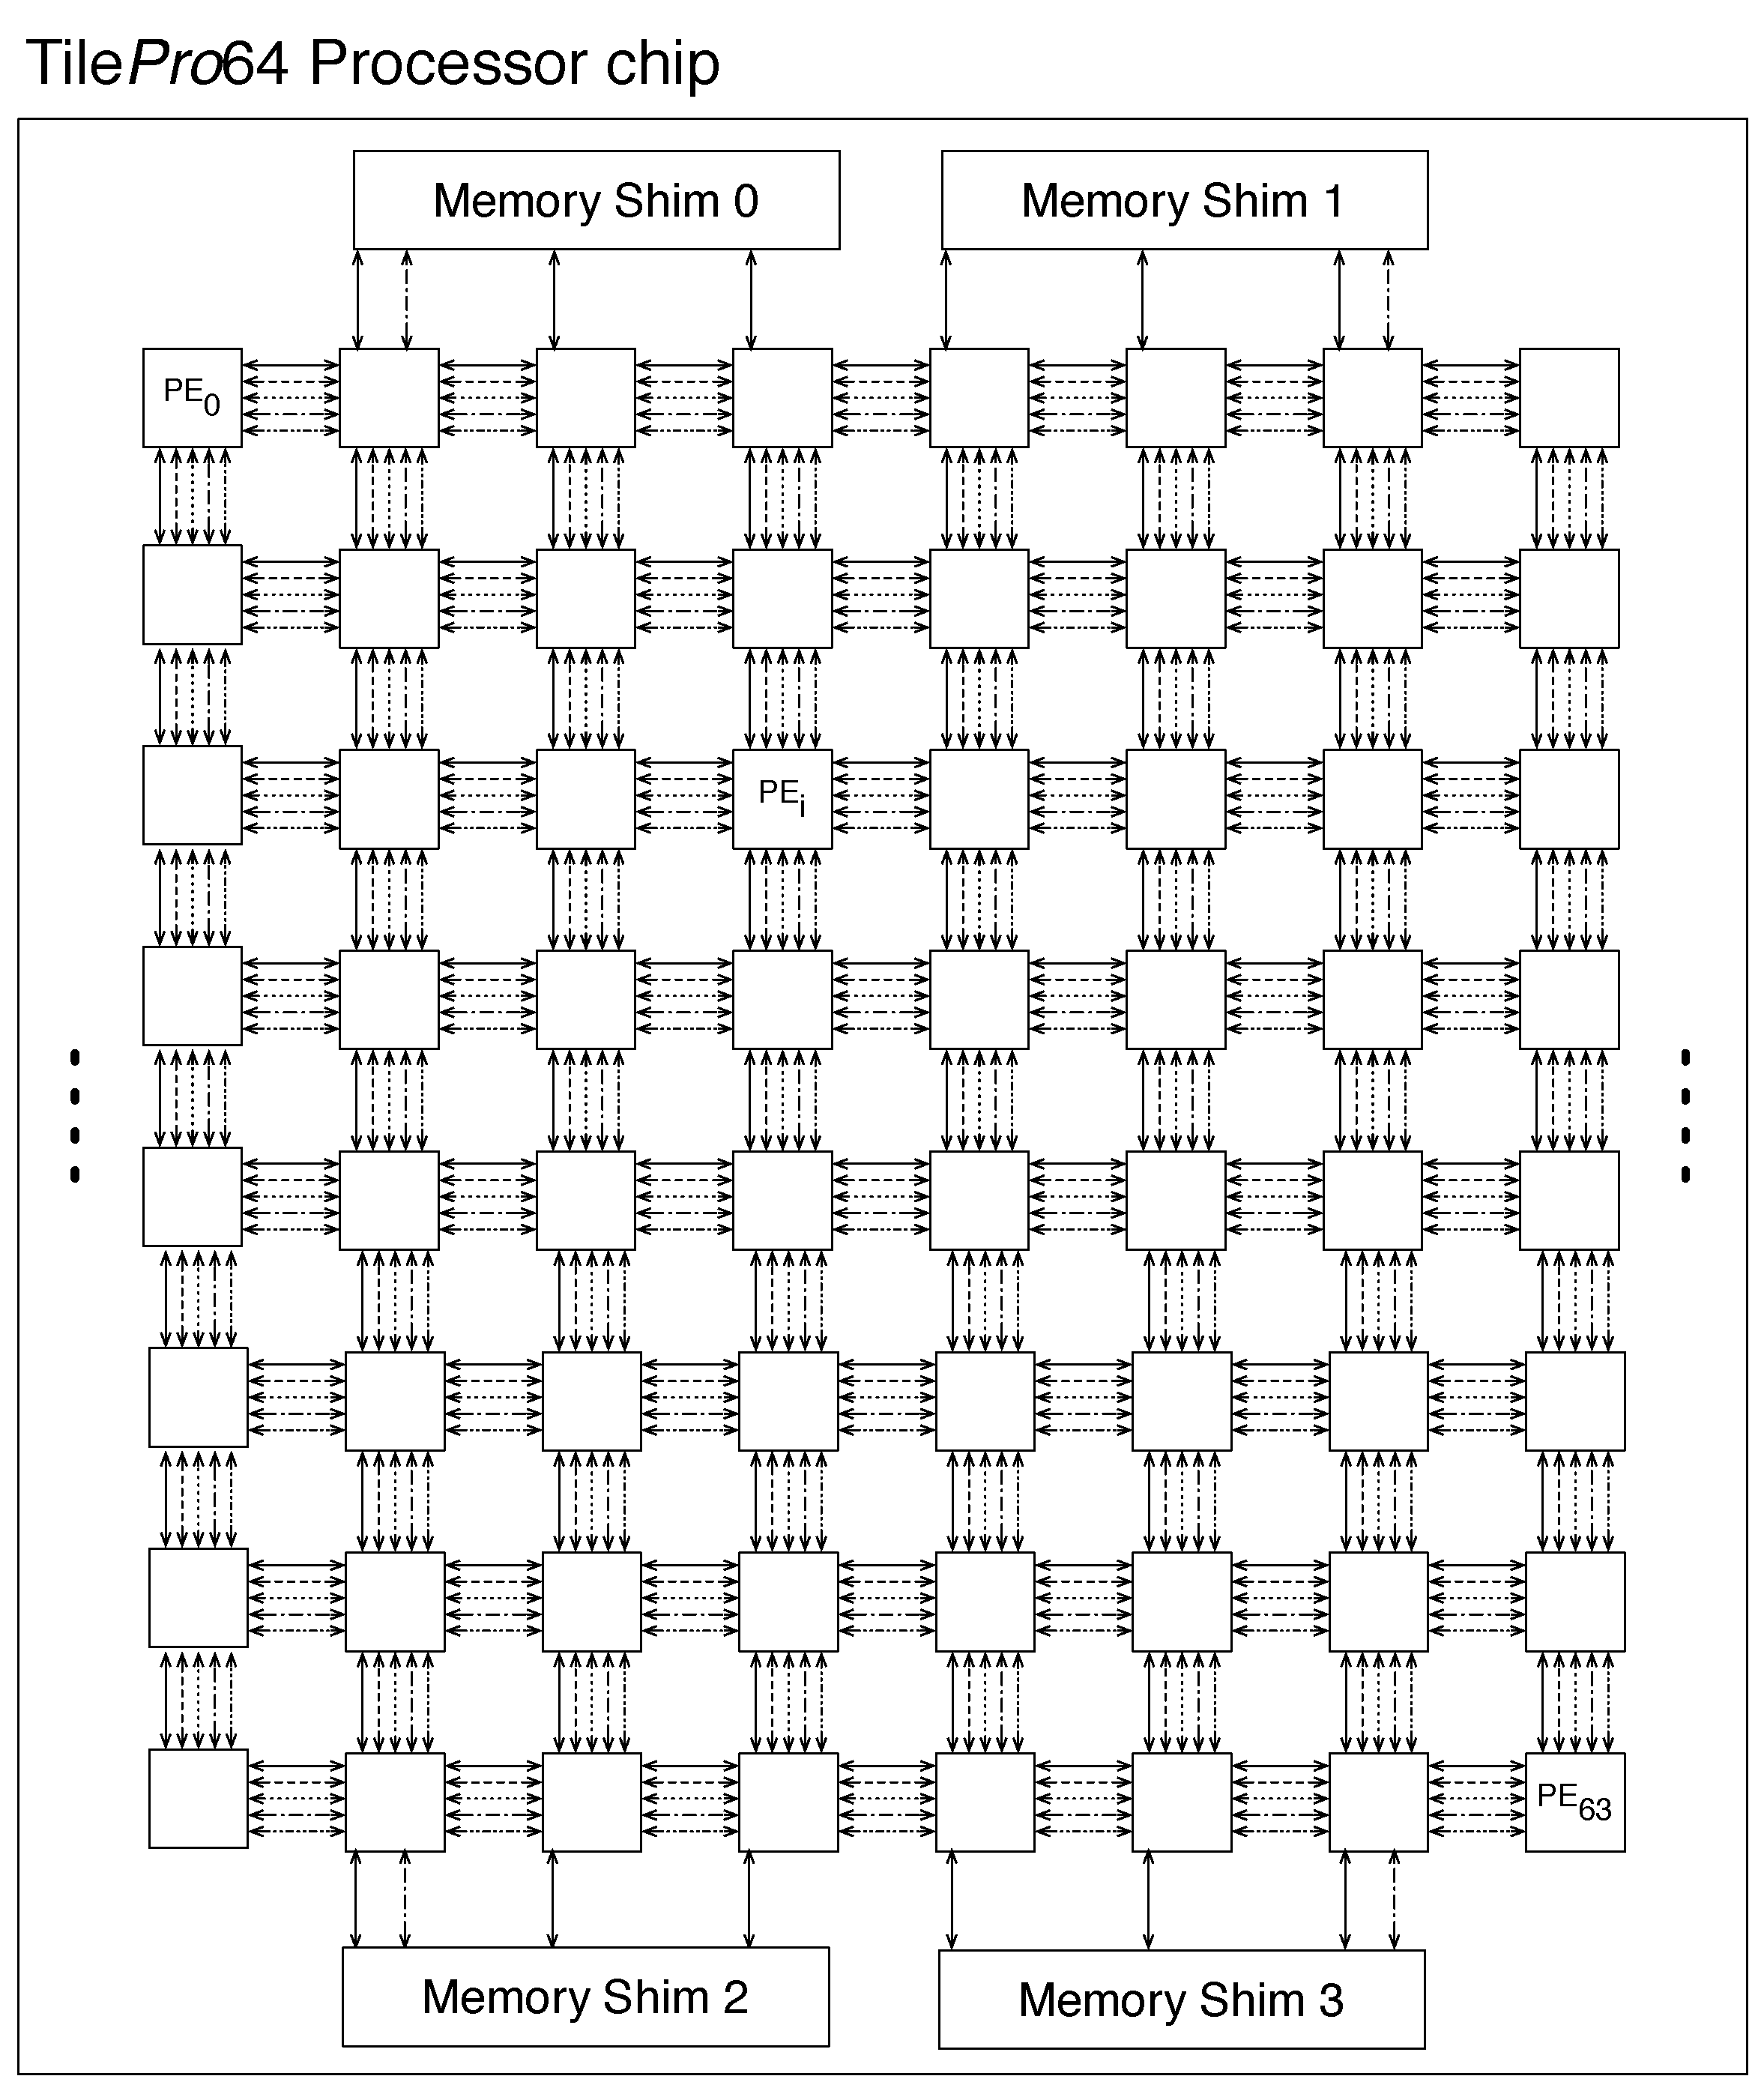
\includegraphics{schema_iMesh.pdf}}
    \label{fig:iMesh}
  \end{subfigure}
  \hspace{1ex}
  \begin{subfigure}[b]{.5\textwidth}
    \centering
    \resizebox{\columnwidth}{!}{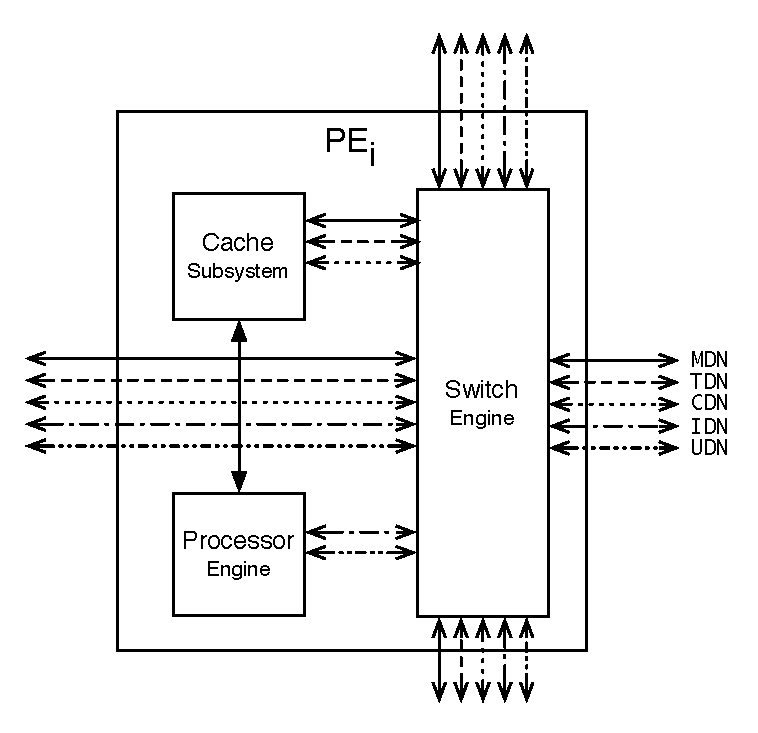
\includegraphics{schema_iMesh_tile.pdf}}
    \label{fig:iMesh_tile}
  \end{subfigure}     
  \caption[Schema del processore Tilera \tile]{Rappresentazione parziale del processore \tile\ con il dettaglio dell'architettura di un singolo Processing Element}
  \label{fig:tilera}
\end{figure}

\subsubsection{User Dynamic Network}
\label{sct:intro_arch_udn}
La UDN \`e collegata direttamente tra CPU e l'unit\`a di switching del PE. Sono disponibili quattro flussi UDN, nella CPU esistono altrettante code verso le quali sono direzionati i pacchetti del flusso corrispondente; esiste inoltre una quinta coda, detta Catch-All, per qualsiasi altro flusso diverso dai quattro precedenti. Le code di demultiplexing UDN sono collegate direttamente alla Unit\`a di Esecuzione delle Istruzioni della CPU. L'accesso ai flussi UDN avviene tramite letture o scritture a 4 registri generali riservati alla UDN. Il programmatore ha possibilit\`a di uso della UDN per mezzo della libreria C messa a disposizione da Tilera, tuttavia, le vere richieste di scrittura e lettura alla UDN sono effettuate per mezzo di istruzioni assembler, come mostrato nel codice~\ref{lst:udn_eg}.
%% udn0 - udn3 <----> 59 - 62
\begin{lstlisting}[float = b, basicstyle = {\small \ttfamily}, commentstyle={\rmfamily \itshape \footnotesize}, caption = {Istruzioni assembler per accedere alla UDN}, label = {lst:udn_eg}]
add r59, r5, r6 // Somma r5 a r6 e invia il risultato 
                // sul primo flusso UDN
add r5, r6, r60 // leggi una parola dal secondo flusso UDN,
                // sommala a r6 e scrivi il risultato in r5
\end{lstlisting}
L'attesa in seguito all'invocazione di un invio, o di una ricezione, \`e caratterizzata da un basso consumo di energia e da zero latenza alla sveglia. Si osserva che l'attesa in ricezione avviene quando non esistono dati nella coda del flusso UDN specificato. \`E possibile anche l'attesa in seguito all'invio quando la rete non \`e in grado di consumare immediatamente il pacchetto.

In conclusione la rete UDN offre molti vantaggi (bassissima latenza nella comunicazione PE-to-PE, zero latenza nella sveglia, bassi consumi) e presenta alcune limitazioni (il firmware realizza quattro flussi, la dimensione massima dei pacchetti \`e fissata a circa 118 parole). Tale servizio pu\`o perci\`o risultare interessante, e la documentazione ufficiale Tilera lo precisa \cite{ug205}, per ottimizzare l'implementazione di operazioni critiche per le prestazioni, mentre \`e raccomandato l'uso della memoria condivisa per la maggior parte delle comunicazioni. Nel caso di computazioni di grana fine, i meccanismi chiave sono quelli di sincronizzazione e comunicazione tra processi, la cui ottimizzazione fornisce miglioramenti notevoli alle prestazioni.

\subsection{Architettura della memoria principale}
\label{sct:intro_arch_memory}
Esistono quattro controllori della memoria principale collegati ai PE sul bordo superiore e inferiore della mesh. Le pagine di memoria condivisa hanno dimensione 64KB e sono allocate in modo interleave, in parti di 8KB, nei controllori di memoria (``stripped main memory mode''), tale configurazione rende uniforme l'accesso ai controllori di memoria bilanciando il carico di richieste. \`E possibile configurare l'allocazione delle pagine in specifici controllori. \tile\ definisce un modello \emph{rilassato} di consistenza della memoria, in altre parole l'ordinamento delle operazioni di store non \`e totale. Valgono le seguenti due propriet\`a:
\begin{itemize}
  \item la sequenza delle istruzioni originale del programma pu\`o essere modificata a tempo di compilazione, come risultato di ottimizzazioni. 
\item le operazioni di store eseguite da un PE appaiono visibili simultaneamente a tutti gli altri PE, ma possono diventare visibili al PE che ha emesso la scrittura prima che avvenga la visibilit\`a globale.
\end{itemize}       
L'architettura mette a disposizione un'istruzione di barriera di memoria, chiamata anche \emph{memory fence}, la quale stabilisce un ordinamento tra le istruzioni di memoria, altrimenti non ordinate: le operazioni di memoria nel programma prima dell'istruzione barriera di memoria, sono rese globalmente visibili prima di qualsiasi operazione dopo la barriera di memoria.

\subsection{Architettura del sottosistema di memoria cache}
\label{sct:intro_arch_cache}
La cache L1 \`e divisa nella parte istruzioni (L1i) e nella parte dati (L1d), la prima ha dimensione 16KB con blocchi di 64B, la seconda ha dimensione 8KB con blocchi di 16B. L'allocazione dei blocchi nelle due parti L1 avviene solo fault in lettura, le scritture sono write through. La cache L2 ha dimensione 64KB, blocchi di 64B e l'allocazione dei blocchi avviene con fault sia in lettura che in scrittura; la politica di scritture \`e write back.

La coerenza della memoria cache \`e garantita automaticamente, per mezzo del firmware della macchina. \`E possibile configurare la macchina in diverse modalit\`a:
\begin{itemize}
\item memoria coerente nelle cache;
\item memoria non coerente nelle cache, \`e onere del programmatore dell'applicazione garantire la coerenza mediante operazioni di flush e di deallocazione (\`e definita solo una primitiva che invalida il blocco nel PE che ha eseguito la primitiva stessa);
\item non uso della gerarchia cache.
\end{itemize}
La coerenza automatica si basa su invalidazione, l'implementazione \`e \emph{Directory-based}. In particolare la tabella Directory \`e implementata in modo distribuito nei PE della macchina.
Per un certo blocco di cache $b$ viene usato il termine Home con il consueto significato nei protocolli di coerenza cache: il PE che \`e Home per il blocco $b$ detiene e gestisce le informazioni di coerenza della cache di $b$, e invia messaggi di invalidazione quando necessario. Un PE gestisce la coerenza, e contiene le entrate della directory, dei soli blocchi di cui \`e Home. 
Nell'architettura Tilera un PE Home per un certo blocco $b$ ha anche la caratteristica di possedere sempre la copia aggiornata di $b$ nella propria L2 (in un protocollo di coerenza tale PE verrebbe chiamato Owner di $b$ oltre che Home). Questo consente di poter vedere un terzo livello di cache distribuito sulle L2: se un PE esegue una lettura da memoria che risulta miss sia nella L1d che nella L2 locali, tale richiesta viene inoltrata al PE che \`e Home del blocco corrispondente, piuttosto che essere inviata direttamente alla memoria. \`E onere della L2 di tale PE rispondere alla richiesta: se il blocco \`e allocato allora viene inviata immediatamente la risposta contenente il valore del blocco, altrimenti viene inoltrata la domanda di trasferimento alla memoria principale, e successivamente il messaggio di risposta al PE richiedente. Ne segue una caratterizzazione dei due livelli di cache: L1 \`e una cache privata per la propria CPU, la L2 \`e una cache condivisa con gli altri PE, in quanto pu\`o contenere sia blocchi acceduti dalla CPU locale, che blocchi di cui \`e Home e per i quali ha ricevuto una richiesta da un altro PE.
 
Lo schema con cui i blocchi di memoria vengono associati ai PE Home \`e dinamico e pu\`o essere controllato dal programmatore in modo da ottimizzare la specifica computazione, ad esempio rendendo massima la localit\`a delle informazioni nei PE. Sono disponibili tre modi per definire l'homing:
\begin{description}
\item [Local Homing] \`e la modalit\`a predefinita per lo stack dei processi e threads. Una pagina di memoria \`e Home nel PE che ha effettuato l'accesso. Ne segue che in tale modalit\`a tutti gli accessi sono diretti ai controllori di memoria e non viene usato il meccanismo di L3 cache distribuito nelle cache L2 degli altri PE. Ci\`o \`e utile per dati privati in quanto non trarrebbero vantaggio dall'uso della cache di una altro PE come L3.
\item [Hash-for-Home] \`e la modalit\`a predefinita per tutti gli altri dati del processo. Una pagina di memoria viene homed in modo sparso nei PE della macchina con granularit\`a di un blocco L2. Tale dispersione delle pagine di memoria nella cache dei PE consente una distribuzione uniforme del traffico nelle reti del chip e un effettivo bilanciamento del traffico di richieste alla memoria tra l'insieme dei PE.
\item [Remote Homing] per una generica pagina di memoria viene impostato il corrispondente PE Home. Tale PE \`e anche chiamato L3 per la pagina. Le richieste di accesso ad un qualsiasi blocco interno alla pagina, da parte di altri PE, vengono inoltrate al PE Home; quest'ultimo ha l'onere di rispondere con il trasferimento del blocco, eventualmente effettuando l'accesso alla memoria principale se il blocco non \`e presente nella sua L2. Tale configurazione \`e utile con strutture dati condivise, il cui accesso avviene con uno schema produttori-consumatore. Configurare la pagina dell'oggetto in questione come Home nel PE che esegue il consumatore aumenta la localit\`a degli accessi di tale processo, il quale si trova direttamente nella propria L2 la struttura modificata dai produttori. Le scritture effettuate dai produttori, infatti, sono write through nella cache del PE Home.
\end{description}



\newpage
\FloatBarrier
\section{Specifica dei meccanismi di comunicazione}
\label{sct:specifica_meccanismi}

I meccanismi di message passing presi in considerazione sono canali unidirezio\-nali di forma simmetrica e asimmetrica in ingresso, entrambi con grado di asincronia unitario e tipo di dati trasmessi ``riferimento alla memoria condivisa''. \\
Viene fornita una descrizione astratta di questi meccanismi e delle relative primitive. Nelle sezioni successive sono descritte le implementazioni che fanno uso di due diversi supporti architetturali: la memoria condivisa con l'uso della gerarchia cache, e la rete di interconnessione tra i PEs. 

\subsection{Descrizione dei canali al livello firmware}
\label{sct:ch_firmware}
Prima di descrivere l'implementazione delle forme di comunicazione considerate, viene descritto brevemente il protocollo tipico per realizzare la comunicazione di unit\`a di elaborazione firmware in modo indipendente dal tempo \cite{vanneschi2009architettura}. Le idee alla base di questo protocollo sono utilizzate per realizzare dei meccanismi efficienti e ottimizzati sull'architettura di \tile.
\begin{figure}[!b]
  \begin{subfigure}[b]{.5\textwidth}
    \centering
    \resizebox{.8\columnwidth}{!}{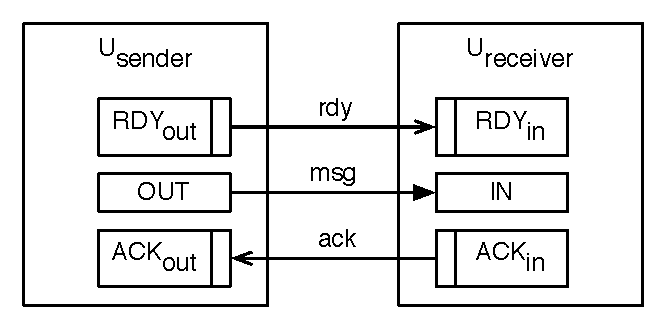
\includegraphics{firmware_communication.pdf}}
    \caption{Comunicazione simmetrica}
    \label{fig:fwcomm_sym}
  \end{subfigure}
  \begin{subfigure}[b]{.5\textwidth}
    \centering
    \resizebox{.8\columnwidth}{!}{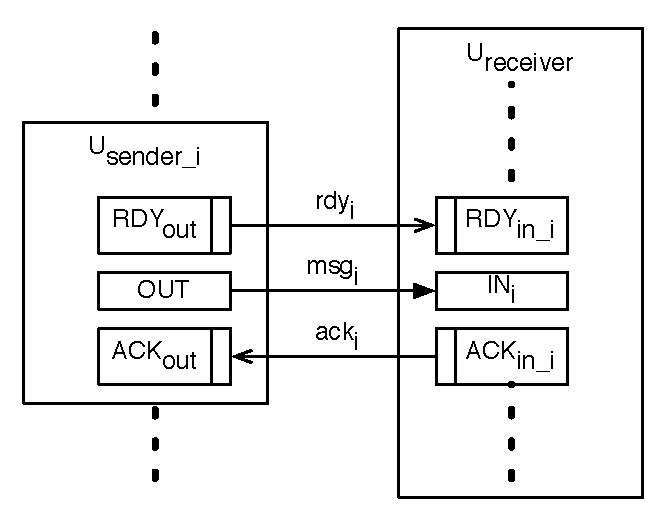
\includegraphics{firmware_asym_comm.pdf}}
    \caption{Comunicazione asimmetrica}
    \label{fig:fwcomm_asym}
  \end{subfigure}
  \caption{Componenti di un canale di comunicazione firmware}
  \label{fig:fwcomm}
\end{figure}

Si consideri la comunicazione simmetrica, il protocollo definisce due eventi: ``la presenza di un messaggio nel canale'' e ``la ricezione del messaggio da parte del ricevente''; nel livello firmware tali eventi sono realizzati tramite due collegamenti di un bit detti di Ready (Rdy) e di Acknowledgement (Ack) e da una coppia di indicatori di interfaccia per ciascun collegamento. Un canale di comunicazione a livello firmware \`e perci\`o costituito da tre componenti: l'interfaccia di uscita, il collegamento fisico e l'interfaccia di ingresso. Le interfacce contengono l'indicatore di uscita, quello di ingresso e il registro di uscita contenente il dato da trasmettere. Il collegamento \`e costituito dalle linee per connettere gli indicatori e i registri delle due interfacce. Un indicatore di interfaccia di uscita mette a disposizione l'operazione \emph{set} che provoca l'assunzione del valore 1 nell'indicatore di interfaccia di ingresso ad esso collegato. Un indicatore di interfaccia di ingresso mette a disposizione l'operazione \emph{test} con la quale viene letto il valore dell'indicatore, e l'operazione \emph{reset} con l'esecuzione della quale viene impostato a 0 il valore di uscita dell'indicatore stesso. Considerando due unit\`a $\mathrm{U}_{\mathrm{sender}}$ e $\mathrm{U}_{\mathrm{receiver}}$ collegate dai collegamenti \emph{rdy(1)}, \emph{msg(L)}, \emph{ack(1)} come in figura \ref{fig:fwcomm_sym}, il protocollo di comunicazione \`e perci\`o definito come in codice~\ref{lst:sym_firmware}
\begin{lstlisting}[language={}, morekeywords={msg, vtg}, float=t, caption={Descrizione astratta del protocollo di comunicazione del canale firmware simmetrico}, label={lst:sym_firmware}]
$\mathtt{U}_{\mathtt{sender}}$:send ::
  wait until $\mathtt{ACK}_{\mathtt{out}}$.test() is equal to 1
  send message msg to receiver and
    do $\mathtt{RDY}_{\mathtt{out}}$.set() and 
    do $\mathtt{ACK}_{\mathtt{out}}$.reset()

$\mathtt{U}_{\mathtt{receiver}}$:receive ::
  wait until $\mathtt{ACK}_{\mathtt{in}}$.test() is equal to 1
  use msg received and 
    do $\mathtt{ACK}_{\mathtt{in}}$.set() and
    do $\mathtt{RDY}_{\mathtt{in}}$.reset()
\end{lstlisting}

Il protocollo di comunicazione del canale asimmetrico in ingresso segue da quello descritto nel caso simmetrico: dal punto di vista logico \`e come se venissero adottati tanti canali simmetrici quante sono le unit\`a mittenti, ogni canale collega una unit\`a mittente all'unit\`a destinataria, figura \ref{fig:fwcomm_asym}. Il comportamento della funzione di invio rimane invariato rispetto a quello descritto precedentemente. Quello della funzione di ricezione testa tutti gli indicatori di tipo Rdy e con una certa politica ne seleziona uno tra quelli attivi ed esegue il protocollo del caso simmetrico, leggendo il valore, resettando il Rdy e inviando l'ack per il canale scelto.


\newpage
\subsection{Specifica dei canali di comunicazione}
\label{sct:specif_meccanismi_intro}
\begin{figure}[!t]
  \begin{subfigure}[b]{.5\textwidth}
    \centering
    %% \resizebox{\columnwidth}{!}{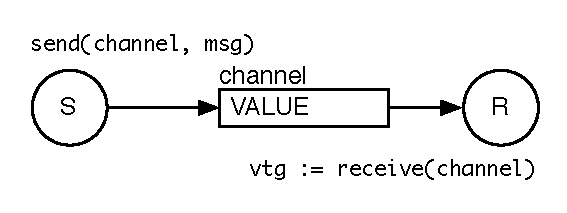
\includegraphics{abstract_sym.pdf}}
    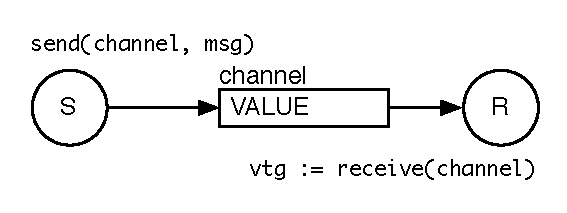
\includegraphics[scale=.5]{abstract_sym.pdf}
    \caption{Canale simmetrico}
    \label{fig:abstract_channel_sym}
  \end{subfigure}
  \begin{subfigure}[b]{.5\textwidth}
    \centering
    %% \resizebox{\columnwidth}{!}{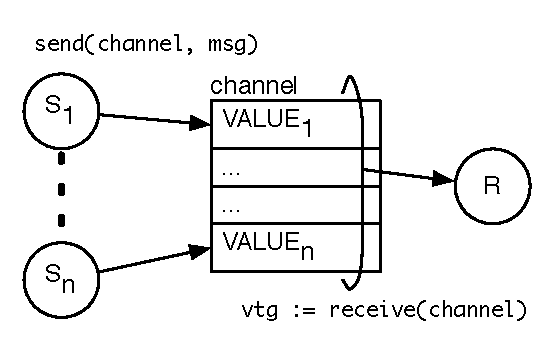
\includegraphics{abstract_asym.pdf}}
    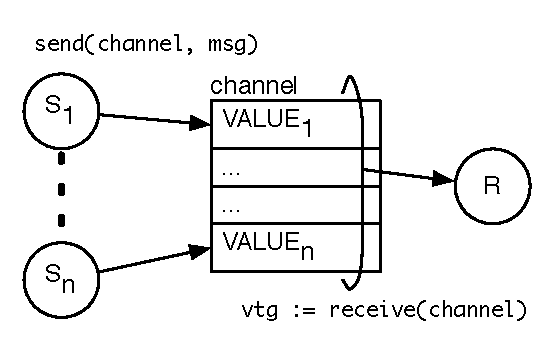
\includegraphics[scale=.5]{abstract_asym.pdf}
    \caption{Canale asimmetrico in ingresso}
    \label{fig:abstract_channel_asym}
  \end{subfigure}
  \caption[Canali di comunicazione tra processi]{Rappresentazione astratta di canali con grado di asincronia unitario}
  \label{fig:abstract_channels}
\end{figure}

%% >>>> INTRODUZIONE
%% ---> TODO
%% Si desidera implementare meccanismi di \emph{fast} message passing, in particolare canali di comunicazione simmetrici e asimmetrici in ingresso con grado di asincronia 1 e tipo di dato ``riferimento''. Si applica la copia del valore del messaggio nel canale.

%%Al fine di poter offrire un supporto efficiente ai paradigmi di programmi paralleli caratterizzati da grana fine sia nelle computazioni nei processi che nelle comunicazioni tra processi \`e stata studiata l'implementazione di meccanismi di \emph{fast} message passing nel CMP \tile. Meccanismi di questo tipo sono caratterizzati da una bassa latenza di comunicazione, 

%% Le forme di comunicazione che sono espresse da tali meccanismi sono sufficienti per fornire il supporto dei principali paradigmi di programmazione parallela. Il grado di asincronia unitario risulta sufficiente per le forme di parallelismo e consente minori overhead nell'implementazione dei meccanismi rispetto a gradi di asincronia maggiori di uno.

%% >>>> DESCRIZIONE DEI MECCANISMI
Con canale di comunicazione si intende il collegamento logico tramite il quale due o pi\`u processi comunicano. L'astrazione di canale come meccanismo primitivo di scambio di informazioni tra processi viene fornita dal supporto a tempo di esecuzione della nostra libreria. Il canale \emph{simmetrico} \`e un oggetto che mette in comunicazione un processo mittente con un processo destinatario, consentendo l'invio di messaggi dal processo mittente al processo destinatario. Un canale \emph{asimmetrico in ingresso} \`e un oggetto che mette in comunicazione pi\`u processi mittenti con un singolo processo destinatario, consentendo a ciascun mittente l'invio di messaggi al processo destinatario. Il destinatario riceve i messaggi in modo non deterministico e senza saperne la provenienza, a meno di comunicazioni esplicite. 

Per entrambi i canali sono definite due primitive di comunicazione, quella di invio e quella di ricezione le quali sono usate rispettivamente dal processo mittente e dal processo destinatario del canale di comunicazione. Si considera la seguente dichiarazione C delle primitive:
\begin{lstlisting}[morekeywords={ch_sym_t, ch_asym_t}]
void sym_send(ch_sym_t *ch_descr, const void *msg)
void *sym_receive(ch_sym_t *ch_descr)

void asym_send(ch_asym_t *ch_descr, const void *msg, int rank)
void *asym_receive(ch_asym_t *ch_descr)
\end{lstlisting}
Ad ogni primitiva viene quindi passato, come primo parametro, il descrittore di canale come riferimento ad una struttura dati allocata in memoria condivisa. Non viene usata la tecnica zero-copy in quanto non \`e applicabile all'implementazione che fa uso della UDN. La primitiva di invio ha come secondo parametro il valore del messaggio, quella di ricezione ritorna il valore letto dal canale come valore di ritorno, il valore del messaggio \`e copiato prima nel canale poi nella variabile targa. Nel caso asimmetrico \`e necessario specificare alla primitiva di invio l'identificatore del mittente all'interno del canale, ci\`o \`e necessario per l'implementazione, come spiegato nelle sezioni successive per entrambi i supporti.

%% >>>> SPECIFICA PRIMITIVE DI COMUNICAZIONE
Si considera il seguente comportamento ad alto livello delle due forme di comunicazione con il grado di asincronia considerato:
%% Si considerano le seguenti specifiche del comportamento della primitiva di invio su un canale simmetrico con grado di asincronia unitario:
\begin{description}
\item [canale simmetrico con grado di asincronia unitario] prevede che il processo mittente possa inviare fino ad un messaggio senza attendere che il destinatario lo abbia ricevuto. Nel caso in cui il mittente intenda inviare un secondo messaggio senza che il destinatario abbia ricevuto quello precedente occorre che il mittente attenda la ricezione da parte del destinatario.
\item [canale asimmetrico in ingresso con grado di asincronia unitario] \hfill ogni processo mittente pu\`o inviare fino ad un messaggio senza attendere che il destinatario lo abbia ricevuto. Nel caso in cui un generico mittente intenda inviare un secondo messaggio senza che il destinatario abbia ricevuto il messaggio precedentemente inviato dal quello specifico mittente, occorre che tale mittente attenda la ricezione da parte del destinatario del messaggio precedente. 
\end{description}
Per quanto riguarda il comportamento del ricevente di un canale asimmetrico, non si impone una specifica politica di ricezione. Il comportamento che pu\`o essere considerato naturale \`e la ricezione FIFO dei messaggi inviati dai mittenti, tuttavia tale funzionamento non \`e imposto. Si pu\`o infatti parlare del canale asimmetrico in ingresso come un caso particolare di comportamento non deterministico del destinatario nella ricezione da pi\`u canali simmetrici.

\begin{lstlisting}[
    float = b,
    caption = {Descrizione astratta del protocollo di comunicazione per un canale simmetrico con grado di asincronia 1}, 
    label = lst:abstract_sym_protocol,
    morekeywords={msg, vtg, ready, acknowledgement, sender, receiver}
]
send ::
  wait until acknowledgement signal is received
  send the message to receiver and
    reset acknowledgement flag and
    signal ready to the receiver
  
receive ::
  wait until ready signal is received
  copy the message received from sender into vtg and
    reset ready flag and
    signal acknowledgement to the sender
\end{lstlisting}
Nelle sezioni successive verranno descritte le implementazioni dei due tipi di canale che sfruttano supporti architetturali diversi. I protocolli di comunicazione che costituiscono l'implementazione con i diversi supporti fanno riferimento al protocollo usato al livello firmware per la comunicazione di due unit\`a di elaborazione indipendente dal tempo. Tale protocollo \`e chiamato nel seguito Rdy-Ack. Descriviamo qui, in modo astratto, le azioni dei processi comunicanti definite dal protocollo che assicurano la correttezza della comunicazione, ovvero: 
\begin{itemize}
\item non si verifica mai la perdita di un messaggio,
\item se il/un processo mittente invia un messaggio allora prima o poi il processo destinatario lo deve ricevere,
\item se il processo destinatario riceve un messaggio allora prima o poi il processo mittente che ha effettuato l'invio di quel messaggio deve essere in grado di inviarne un altro.
\end{itemize}
%% >>>> DESCRIZIONE DEL PROTOCOLLO
Per il canale simmetrico si hanno le azioni delle due entit\`a descritte nel codice~\ref{lst:abstract_sym_protocol}. Il canale asimmetrico in ingresso ha protocollo simile, in quanto pu\`o essere visto come costituito da tanti canali simmetrici Rdy-Ack quanti sono i mittenti, dove ogni canale collega un mittente al destinatario. Il comportamento dell'invio di un messaggio \`e esattamente lo stesso di quello adottato nel canale simmetrico, mentre la ricezione ha l'onere di scegliere in modo non deterministico un canale da cui ricevere tra i canali pronti.



%% che il \emph{mapping} delle applicazioni parallele considerate nell'architettura \`e di \emph{tipo esclusivo}, ovvero esiste una corrispondenza biunivoca tra ogni processo dell'applicazione e il processore della macchina che lo esegue. 
%% ---> MOTIVAZIONI

\newpage
\FloatBarrier
\subsection{Implementazione dei canali con memoria condivisa}
\label{sct:specifica_sm}
Sfruttando la memoria condivisa si ha una implementazione semplice e lock-free delle comunicazioni simmetrica e asimmetrica con il protocollo Rdy-Ack. Ci\`o \`e determinato dal fatto che non esiste un buffer o altre strutture dati sulle quali i processi devono accedere in modo indivisibile. L'adozione di un grado di asincronia unitario e la sincronizzazione tramite gli eventi Rdy e Ack permette di effettuare accessi al descrittore del canale senza la necessit\`a di mutua esclusione.

\subsubsection{Comunicazione simmetrica}
\label{sct:sym_sm_rdyack}
Si considera la comunicazione simmetrica: il descrittore di canale \`e costituito da tre informazioni:
\begin{inparaenum}[\itshape a~\upshape)] 
\item il valore di Rdy, \item il valore di Ack, \item il valore del messaggio.
\end{inparaenum}
Ogni informazione \`e allocata in una parola, in particolare abbiamo la seguente definizione del descrittore di canale:  i flag di Rdy e di Ack sono di tipo intero, il messaggio \`e di tipo riferimento.
\begin{lstlisting}
struct ch_sym_sm_rdyack_t { 
  int rdy; 
  int ack; 
  void *value;
};
\end{lstlisting}
La segnalazione di un evento di Rdy o di Ack avviene impostando al valore 1 il corrispondente campo nel descrittore di canale. L'attesa attiva di un processo sul canale \`e realizza con la strategia \emph{retry} sul valore del flag Rdy o Ack: si continua a testare il valore del flag fino a quando non assume valore 1.
Il protocollo di comunicazione viene perci\`o realizzato con le seguenti azioni:
\begin{lstlisting}[
        morekeywords={rdy, ack, value},
        caption={Descrizione astratta del protocollo di comunicazione Rdy-Ack su memoria condivisa},
        label={lst:abstr_mem_sym}
]       
send(ch_descr, msg) ::
  wait until ch_descr->ack flag is equal to 1;
  reset ch_descr->ack flag to 0;
  copy msg into ch_descr->value entry;
  memory_fence();
  set ch_descr->rdy flag to 1;

receive(ch_descr) ::
  wait until ch_descr->rdy flag is equal to 1;
  reset ch_descr->rdy flag to 0;
  read the ch_decsr->value entry;
  set ch_descr->ack flag to 1;
\end{lstlisting}
La mutua esclusione nell'uso del valore del canale da parte dei processi mittente e destinatario \`e garantita dalla sincronizzazione dei due processi sui due valori di Rdy e Ack: ogni processo accede al valore del canale solo dopo che il processo partner ha notificato tale possibilit\`a. Per garantire la correttezza della comunicazione \`e quindi sufficiente adottare la seguente condizione iniziale:
\begin{itemize}
\item all'avvio dell'applicazione tutti i canali devono avere descrittore con campo Ack inizializzato ad 1 e capo Rdy inizializzato a 0.
\end{itemize}
Tale condizione iniziale, insieme all'adozione del protocollo, garantisce la seguente propriet\`a:
\begin{itemize}
\item ogni notifica di evento Rdy o Ack trova sempre l'evento corrispondente precedentemente falso.
\end{itemize}

%% L'IMPLEMENTAZIONE \`E LOCK-FREE, NECESSARIA MEMORY FENCE
Il fatto che sia possibile evitare l'uso di meccanismi di lock per l'esecuzione indivisibile del codice \`e un aspetto positivo dell'implementazione con memoria condivisa del protocollo Rdy-Ack, in quanto si evitano i relativi overhead sulle prestazioni. Al fine di garantire la correttezza \`e tuttavia richiesto l'uso di scritture sincrone alla memoria condivisa. \`E necessario che le scritture effettuate dal mittente sul valore del canale e sul flag di Rdy siano viste dal destinatario nello stesso ordine. Come descritto in sezione~\ref{sct:intro_arch_memory}, \tile\ adotta un modello rilassato di consistenza della memoria, sia per quanto riguarda l'ordinamento di istruzioni all'interno di una CPU, sia per l'atomicit\`a delle scritture in memoria condivisa. Ci\`o rende necessario l'uso di una barriera di memoria tra le due scritture effettuate dal mittente (riga 5 del codice~\ref{lst:abstr_mem_sym}), in modo che la scrittura del valore 1 sul flag Rdy sia sempre vista dal processo destinatario dopo la scrittura del messaggio nel canale. Il comportamento sincrono delle scritture in memoria, indotto dall'uso della barriera, produce overheads aggiuntivi rispetto al comportamento asincrono delle scritture. La barriera della memoria, e la corrispondente degradazione delle prestazioni, pu\`o essere eliminata con l'adozione di un protocollo di comunicazione alternativo, come mostrato in sezione~\ref{sct:sym_sm_nullack}.

%% USO SEMPRE LA CACHE
La politica di attesa attiva \emph{retry} \`e caratterizzata da un aumento dei conflitti alla memoria principale. Per evitare ci\`o e ridurre la latenza di sveglia si prendono in considerazione solo implementazioni che fanno uso della gerarchia cache. In tale scenario la prima lettura del valore di un flag causa il trasferimento del blocco corrispondente nei livelli L2 e L1D della cache locale, e le letture successive del valore del flag rimangano interne alla CPU, in quanto servite dalla cache locale. Quando il processo partner esegue la scrittura sul flag il meccanismo di coerenza della cache provvede a notificare il cambiamento e aggiornare il valore nella cache locale.

%% EFFETTO SULLE PRESTAZIONI DELLA COERENZA CACHE
Come descritto in sezione~\ref{sct:intro_arch_cache} il meccanismo di coerenza della cache \`e configurabile in molti aspetti, in particolare \`e possibile impostare il PE Home per una certa pagina di memoria. 
In sezione~\ref{sct:intro_arch_cache} viene spiegato come l'uso della strategia \emph{Remote Homing} sia conveniente in computazioni con singolo consumatore di una struttura dati condivisa, e permetta di evitare l'uso di invalidazioni e conseguenti copie di blocchi.
%, consentendo invece l'attuazione di un modello di programmazione di tipo \emph{remote storing}. 
Di seguito descriviamo il comportamento della comunicazione simmetrica con il protocollo Rdy-Ack e il descrittore di canale presentati, con la configurazione predefinita della coerenza della cache, quindi verr\`a presentata una versione ottimizzata che minimizza i messaggi di coerenza e le copie dei blocchi grazie alla configurazione dei PEs Home e al partizionamento del descrittore del canale nelle cache dei PEs.

%% USO PREDEFINITO DELLA COERENZA CACHE
\begin{figure}[!t]
  \centering
  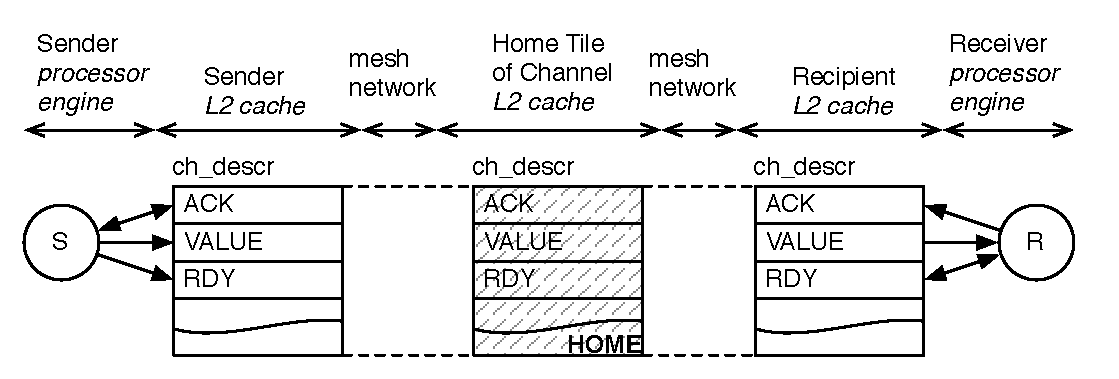
\includegraphics[scale=.5]{cache_sym_sm_no.pdf}
  \caption[Comunicazione simmetrica su memoria condivisa, non ottimizzata]{Rappresentazione di una comunicazione simmetrica tra un processo mittente $S$ e uno destinatario $R$ con uso della memoria condivisa e gestione predefinita della coerenza di cache (hash-for-home strategy)} 
  \label{fig:cache_sym_sm_no}
\end{figure}
La strategia predefinita di allocazione delle pagine di memoria nelle cache \`e \emph{Hash-for-Home} \cite{ug205}. La gestione delle informazioni di coerenza di cache, in particolare l'entrata della Directory, del blocco che contiene il descrittore di canale allocato viene affidata ad un generico processing element $\mathrm{PE}_k$. Durante l'esecuzione del programma parallelo il processo mittente, eseguito in $\mathrm{PE}_i$, e il processo destinatario, eseguito in $\mathrm{PE}_j$, eseguono, per mezzo delle primitive di comunicazione, degli accessi al descrittore di canale. In generale $k \neq i$ e $k \neq j$ quindi si hanno tre copie del blocco contenente il descrittore di canale come mostrato in figura~\ref{fig:cache_sym_sm_no}. La modifica di un campo del descrittore del canale effettuata da uno dei due processi comunicanti provoca l'invalidazione del blocco di L2 nel PE che esegue il processo partner. Quando il PE che contiene il blocco invalidato riferisce il descrittore di canale, l'intero blocco sar\`a trasferito dal PE Home, $\mathrm{PE}_k$, al PE stesso. Nel caso migliore si ha una invalidazione e corrispondente trasferimento di blocco al termine di ogni esecuzione di una primitiva di comunicazione, quando viene notificato un evento di sincronizzazione al processo partner per mezzo di una scrittura nel descrittore di canale.
%% USO OTTIMIZZATO DELLA COERENZA CACHE
\begin{table}[!b]
  \begin{center}
    \begin{tabular}{ | l | l | l | l |}
      \hline
      & Rdy & Ack & Value \\ \hline
      Sender & Write Only & Read and Write & Write Only \\
      Receiver & Read and Write & Write Only & Read Only \\
      \hline
    \end{tabular}
  \end{center}
  \caption[Modalit\`a di accesso ad un canale su memoria condivisa]{Modalit\`a di accesso ai campi del descrittore di canale su memoria condivisa}
  \label{tab:accessi_descr_ch}
\end{table}

Questo offre lo spunto su come ottimizzare l'uso delle cache: la scrittura sul campo del descrittore di canale che implementa un segnale di sincronizzazione dovrebbe essere inoltrata direttamente alla cache del PE che attende il segnale, evitando il trasferimento di un blocco di L2 per la trasmissione di una sola parola. 
%Tale comportamento \`e simile al modello di Remote Store Programming nel quale un processo pu\`o scrivere nella memoria locale di un altro processo.
Questo comportamento \`e possibile in quanto:
\begin{itemize}
\item per ogni campo del descrittore esiste uno solo dei due processi che vi accede in lettura(vedi tabella~\ref{tab:accessi_descr_ch}),
\item \`e possibile impostare il PE Home di un certo blocco di cache L2,
\item come descritto nella sezione~\ref{sct:intro_arch_cache} un PE che \`e Home per un blocco detiene sempre la copia corretta del blocco stesso.
\end{itemize}
%Dato che per ciascun campo del descrittore di canale esiste un unico consumatore (vedi tabella~\ref{tab:accessi_descr_ch}),  \`e possibile applicare alle cache L2 il modello RSP utilizzando la strategia di allocazione Remote Homing del \tile. 
%% Partizionando opportunamente il descrittore di canale e configurando come PE Home quei core nel quale viene eseguito il processo che consuma tali dati, abbiamo come risultato che le scritture a tali dati sono dirette e locali al PE che \`e consumatore dei dati.
Il descrittore di canale viene partizionato in due parti, allocate in blocchi distinti e con diverse configurazioni di Homing:
%\begin{inparaenum}[\itshape1\upshape)] 
\begin{description}
\item [la parte di output] contiene tutti i campi acceduti in lettura del mittente (Ack), ed \`e allocata impostando come PE Home quello che esegue il processo mittente, 
\item [la parte di input] contiene tutti i campi acceduti in lettura dal mittente (Rdy e Value), ed \`e allocata impostando come PE Home quello che esegue il processo destinatario.
\end{description}

Con tale configurazione si incrementa la localit\`a delle informazioni: la coerenza dei dati e l'allocazione degli stessi avviene nella cache del PE che consuma tali dati, permettendo al PE produttore di effettuare scritture direttamente nella cache locale del consumatore tramite messaggi write-through. I processo consumatore dei dati trova le informazioni gi\`a aggiornate direttamente nella cache locale alla CPU che lo esegue. 

Si osserva inoltre che, in tale computazione, il processo consumatore di una informazione esegue anche scritture sul blocco, ci\`o causa l'invio di messaggi di invalidazione del blocco alla cache L2 del PE che esegue il produttore. Tuttavia in futuro non si verificher\`a mai un trasferimento del blocco in quanto il produttore esegue \emph{esclusivamente} scritture sul blocco, ci\`o causa l'allocazione del blocco nella L2 locale (quando il blocco \`e non valido), la modifica della singola parola scritta e l'invio del messaggio Write-Through alla cache L2 del PE consumatore.
\FloatBarrier
\begin{figure}[!t]
  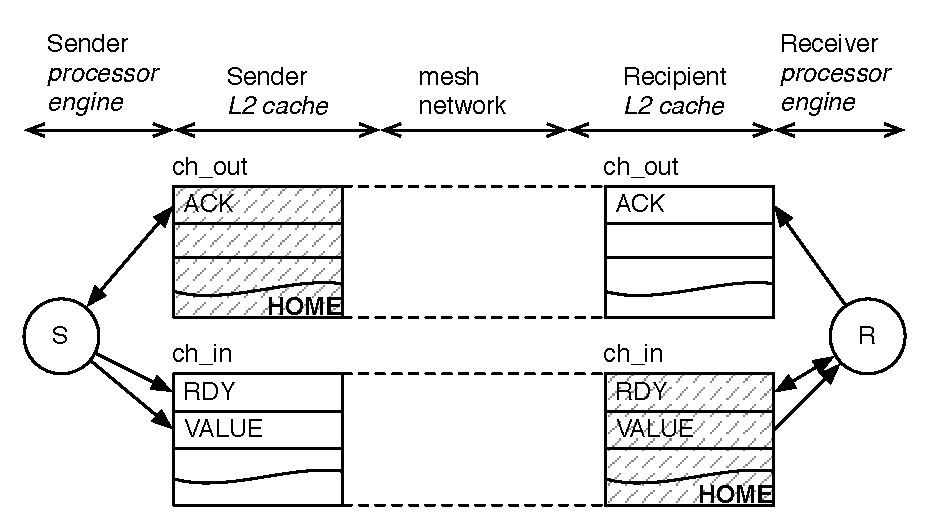
\includegraphics[scale=.5]{cache_sym_sm_fence.pdf}
  \centering
  \caption[Comunicazione simmetrica su memoria condivisa]{Rappresentazione di una comunicazione simmetrica tra i processi $S$ e $R$ con uso della memoria condivisa e gestione ottimizzata della coerenza di cache con strategia Remote Homing per il descrittore di canale}
  \label{fig:cache_sym_sm_fence}
\end{figure}

In conclusione si fa presente che esiste un terzo blocco di cache, usato per il supporto del canale di comunicazione, che contiene i riferimenti alle due parti del descrittore di canale. Tale blocco \`e sempre acceduto in sola lettura, quindi non presenta particolari problemi per le prestazioni e pu\`o essere allocato in uno dei due PE comunicanti con strategia Remote Homing oppure in un terzo PE con strategia Hash-for-Home.

\newpage

\FloatBarrier
\subsubsection{Comunicazione asimmetrica in ingresso}
\label{sct:asymin_sm_rdyack}
Il canale asimmetrico in ingresso \`e visto come costituito da tanti canali simmetrici quanti sono i mittenti. Al fine di ottimizzare le prestazioni non si usa direttamente l'implementazione del canale simmetrico ma si sfruttano comunque i risultati e l'analisi di tale meccanismo, in particolare per quanto riguarda l'allocazione degli oggetti condivisi in cache al fine di garantire la maggiore localit\`a possibile. 

Siano $n$ i processi mittenti del canale, dal punto di vista logico il canale asimmetrico usa $n$ canali simmetrici implementati con il protocollo Rdy-Ack, e perci\`o caratterizzati dal valore della tripla $<Rdy,\; value,\; Ack>$. Come descritto nella sezione \ref{sct:sym_sm_rdyack} i valori di  $Rdy$ e $value$ di un canale simmetrico sono allocati in un blocco che ha per Home il PE che esegue il ricevente mentre $Ack$ ha per Home il il PE che esegue il mittente. Per minimizzare il numero dei blocchi allocati in cache si raggruppa l'insieme dei Rdy e dei valori $\{ <Rdy_i,\; value_i> |\; i \in \{ 1, \dots, n\} \}$ allocandolo come vettore di $n$ coppie $<Rdy,\;value>$ e impostando come Home il PE destinatario, con strategia Remote Homing. I valori di $Ack$ sono invece allocati ciascuno in un blocco che ha per home il PE mittente corrispondente, questo consente la maggior localit\`a possibile. 

Si fa presente che sebbene tale configurazione permetta la massima localit\`a delle informazioni ai PEs, presenta tuttavia l'allocazione nella cache L2 del destinatario di un numero di blocchi che \`e lineare rispetto al numero dei mittenti: si hanno $\frac{2 \cdot 4 \cdot n}{64}$ blocchi necessari a memorizzare l'array di coppie $<Rdy,\;value>$ e $n$ blocchi allocati per le scritture sui flag $Ack$ degli $n$ mittenti. Considerando il caso della comunicazione con il massimo numero (63) di mittenti, si hanno 72 blocchi allocati nel PE destinatario, ovvero uno spazio di 4.5 KB su un totale di 64KB nella cache L2. Dato che siamo interessati a massimizzare le prestazioni si assume che l'uso di tale spazio nella L2 del destinatario non sia problematico per l'applicazione. 

Si osserva che, soprattutto con un numero elevato di mittenti, la sveglia del destinatario sar\`a pi\`u lenta rispetto a quella nel canale simmetrico, infatti l'attesa \`e implementata eseguendo la scansione delle variabili $Rdy$ perci\`o nel caso peggiore \`e necessario effettuare $n$ accessi alla memoria dalla scrittura del valore 1 in un flag $Rdy$ da parte del mittente.

Il descrittore di canale \`e costituito da $n$ riferimenti ai valori di $Ack$ allocati con strategia Remote Homing nei PEs mittenti, e il riferimento alla base del vettore delle coppie $<Rdy, value>$ allocato con strategia Remote Homing nel PE destinatario. Come descritto nella sezione~\ref{sct:specif_meccanismi_intro} il protocollo di comunicazione rimane sosta\-nzialmente invariato rispetto al caso simmetrico, rimane da specificare la politica adottata dal ricevente per selezionare il mittente da cui ricevere tra quelli che hanno inviato un nuovo messaggio. Il supporto della primitiva di ricezione adotta una scansione lineare dell'insieme dei flag $Rdy$ alla ricerca di uno attivo. Ad ogni ricezione viene salvato l'indice del mittente da cui si \`e effettuata la lettura, in modo tale che alla prossima esecuzione della ricezione la scansione dei $Rdy$ si avviata dal mittente successivo. La ricezione \`e quindi non deterministica ed \`e attuata un politica di fairness, sebbene la propriet\`a non sia formalmente soddisfatta. 

Al fine di attuare il protocollo di comunicazione esiste una questione che l'implementazione del supporto della primitiva di invio deve risolvere: conoscere l'identificatore all'interno del canale asimmetrico del mittente che ha eseguito la primitiva. Tale informazione \`e ovviamente indispensabile al protocollo di invio, tra le possibili soluzioni si sono valutate le seguenti due:
\begin{itemize}    
\item la primitiva di invio contiene un terzo parametro, l'identificatore del mittente nel canale, oltre al riferimento al descrittore di canale e al valore del messaggio,
\item ogni mittente usa un proprio descrittore di canale che contiene l'identificatore all'interno del canale, per far ci\`o \`e necessaria una funzione di inizializzazione eseguite da ogni mittente prima dell'avvio della computazione.
\end{itemize}
Si \`e scelta la prima soluzione in quanto anche l'implementazione che sfrutta la UDN verifica lo stesso problema perci\`o \`e assicurata l'uniformit\`a della primitiva di invio nelle due implementazioni del canale asimmetrico. \`E responsabilit\`a dell'utente far si che ogni processo mittente del canale conosca il proprio identificatore univoco all'interno del canale e quindi poter invocare correttamente la primitiva di invio sul canale.
%% 2 * 4 * 64 / 64 + 64 = 8 + 64 = 72 blocchi = 72 * 64 B = 4608 B = 4.5 KB = 1152 word su un totale di 64KB
\begin{figure}[!tb]
  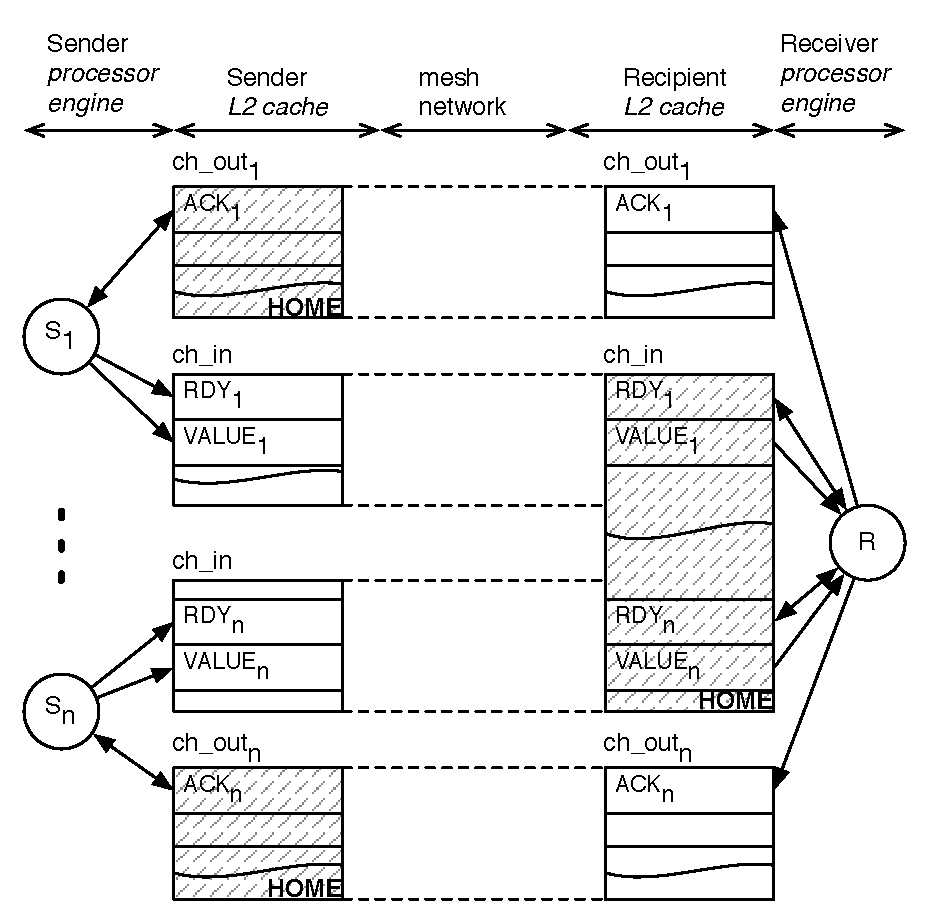
\includegraphics[scale=.5]{cache_asym_sm.pdf}
  \centering
  \caption[Comunicazione asimmetrica su memoria condivisa]{Rappresentazione di una comunicazione asimmetrica tra i processi $\{S_1, \ldots, S_n\}$ e $R$ con uso della memoria condivisa e gestione ottimizzata della coerenza di cache con strategia Remote Homing per il descrittore di canale}
  \label{fig:cache_asym_sm}
\end{figure}

\FloatBarrier
\subsubsection{Comunicazione simmetrica senza barriera di memoria}
\label{sct:sym_sm_nullack}
Nella sezione~\ref{sct:sym_sm_rdyack} si \`e descritta l'implementazione del supporto alla comunicazione simmetrica per mezzo di strutture dati lock-free e, per garantire la correttezza, l'uso della barriera di memoria nel supporto della primitiva di invio. Si propone un'altra possibile implementazione della comunicazione simmetrica con un diverso protocollo che consente il corretto funzionamento con strutture dati lock-free senza l'uso di barriere di memoria. Il protocollo che si va a definire si rif\`a a quello Rdy-Ack, in quanto sono mantenuti gli eventi di sincronizzazione ``messaggio pronto'' (Rdy) e ``messaggio ricevuto'' (Ack). In questo caso l'evento di Rdy non \`e segnalato esplicitamente ma risulta implicito nel cambiamento di valore del canale. Viene infatti definito il valore particolare $\alpha$ che non pu\`o essere assunto dai messaggi trasmessi nel canale e che indica la situazione in cui il canale \`e vuoto. 
Il canale assume valore $\alpha$ all'avvio dell'applicazione e al termine di ogni esecuzione della primitiva di ricezione.
Il flag \verb+Rdy+ \`e eliminato dall'implementazione, il destinatario usa il valore del canale e il valore $\alpha$ per determinare la presenza di un nuovo messaggio, come descritto in codice~\ref{lst:abstr_mem_sym_nullack}. 

Anzitutto si osserva che tale protocollo si applica bene alla nostra implementazione dei canali, in quanto si pu\`o definire, senza perdere di generalit\`a, il valore particolare $\alpha$ come il valore di puntatore ``nullo'': \verb+NULL = (void *) 0+. 
Passando all'analisi della correttezza, la barriera di memoria \`e stata eliminata nella primitiva di invio, in quanto esiste un unico oggetto (il campo \verb+value+) che \`e scritto dal mittente ed \`e acceduto da altri processi.
Nella primitiva di ricezione si hanno invece due oggetti, i campi \verb+value+ e \verb+ack+, che sono scritti dal ricevente ed acceduti dal processo partner. Grazie alla specifica politica di homing di tali oggetti e alla modalit\`a di accesso a questi del processo mittente, l'uso di una memory fence non \`e necessario. Risulta invece sufficiente che il PE che esegue il processo destinatario produca le due scritture nell'ordine specificato. Il campo \verb+value+ ha per Home il PE che esegue il processo ricevente ed \`e acceduto in scrittura dal processo mittente dopo aver letto la variazione di valore del campo \verb+ack+. La prima scrittura \`e quindi locale alla L2 del ricevente, inoltre non ha importanza in che istante diventa visibile agli altri PEs, in quanto l'oggetto scritto (\verb+value+) \`e acceduto in sola scrittura dal mittente. La seconda scrittura \`e una write-through alla L2 del mittente, il quale, una volta letto il nuovo valore pu\`o effettuare una nuova scrittura sul campo \verb+value+ che sicuramente \`e gi\`a stato modificato a \verb+NULL+. Per imporre l'ordinamento delle istruzioni nel PE ricevente si usa l'istruzione \verb+compiler_barrier()+, la quale \`e molto diversa da una barriera di memoria. Il comportamento delle scritture infatti resta asincrono, si \`e solo negato lo spostamento di codice da parte del compilatore, e quindi un ordine diverso di produzione delle due scritture.

\begin{lstlisting}[
        float=t,
        morekeywords={ack, value}, 
        caption={Descrizione astratta del protocollo di comunicazione Null-Ack su memoria condivisa},
        label={lst:abstr_mem_sym_nullack}
]
send(ch_descr, msg) ::
  wait until ch_descr->ack flag is equal to 1;
  reset ch_descr->ack flag to 0;
  copy msg into ch_descr->value entry;

receive(ch_descr) ::
  wait until ch_descr->value is not equal to NULL;
  read the ch_descr->value entry;
  set ch_descr->value to NULL;
  compiler_barrier();
  set ch_descr->ack flag to 1;
\end{lstlisting}

\newpage
\FloatBarrier
\subsection{Implementazione dei canali con UDN}
\label{sct:specifica_udn}
L'uso della UDN permette sia la sincronizzazione dei processi che la trasmissione dei dati tra processi, con latenze molto basse e senza l'utilizzo della memoria condivisa e quindi del sottosistema di cache. A tal fine \`e possibile pensare ad una associazione tra uno o pi\`u canali firmware UDN e un canale software. Esistono per\`o alcune limitazioni imposte da tale rete: 
\begin{itemize}
\item sono disponibili quattro canali UDN (fisici), ciascuno dei quali \`e associato univocamente ad una coda firmware nella CPU, utilizzata in lettura;
\item \`e fissata la massima dimensione dei pacchetti trasmessi nella rete, la quale non pu\`o superare la dimensione delle code firmware nelle CPU.
\end{itemize}
Ne segue che, volendo utilizzare solo la rete di interconnessione senza il supporto della memoria condivisa, il numero di canali software \`e limitato dal numero di canali firmware e che il grado di asincronia di un canale software possa essere limitato dalla dimensione delle code firmware. In altre parole non \`e possibile una implementazione dei canali di comunicazione tra processi che sfrutta esclusivamente UDN e che sia generica, non solo nel grado di asincronia, ma anche nel numero di canali disponibili per processo. Per ottenere tale genericit\`a \`e necessario far uso di memoria condivisa.
\FloatBarrier
\subsubsection{Comunicazione simmetrica}
\label{sct:sym_udn}
\begin{figure}[!b]
  \centering
  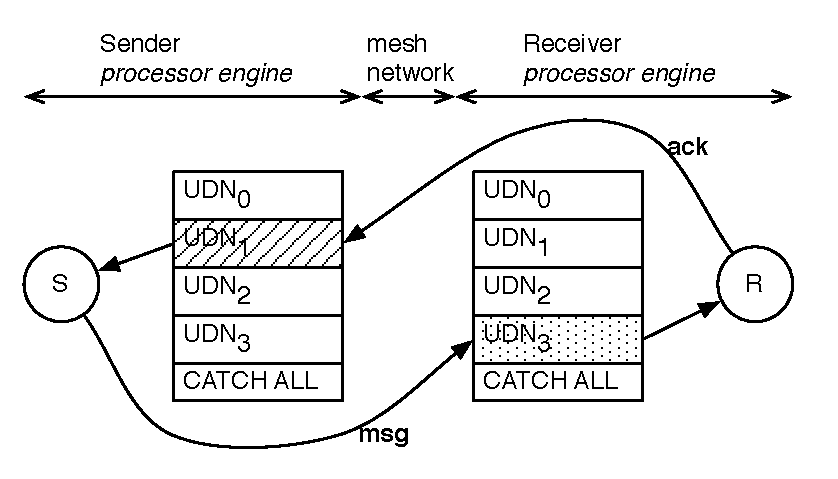
\includegraphics[scale=.5]{udn_sym.pdf}
  \caption[Comunicazione simmetrica su UDN]{Rappresentazione di un possibile scenario di comunicazione simmetrica tra il processo mittente S e quello destinatario R, sfruttando la UDN}
  \label{fig:udn_sym}
\end{figure}
Viene descritta l'implementazione della comunicazione simmetrica che sfrutta in modo ottimale la UDN. 
Tale implementazione pone alcuni limiti sull'utilizzo dei canali ma fornisce le migliori prestazioni possibli riguardo allo scambio dei messaggi sfruttando la UDN. Il protocollo Rdy-Ack per un canale simmetrico viene realizzato impiegando una coda UDN in entrambi i PE che eseguono i processi comunicanti. La coda firmware nel destinatario \`e usata per ricevere i messaggi, il segnale di Rdy \`e implicito con la ricezione di un nuovo messaggio, la coda firmware nel mittente \`e usata per i segnali di Ack, i quali sono esplicitati con l'invio di un messaggio di valore arbitrario di dimensione una parola dal destinatario a tale coda UDN nel mittente. Un possibile scenario \`e mostrato in figura~\ref{fig:udn_sym} dove il canale di comunicazione \`e implementato tramite l'utilizzo della seconda coda UDN nel processo mittente, per la ricezione dei segnali di Ack, e con la quarta coda UDN nel processo destinatario, per la ricezione dei messaggi; ne segue che in entrambi i PE, che eseguono esclusivamente il processo mittente o quello destinatario, rimangono disponibili altre tre code (o canali) UDN utilizzabili per altrettanti canali di comunicazione tra processi. Il protocollo di comunicazione segue quindi lo schema del codice~\ref{lst:abstr_udn_sym}: viene usata una struttura dati condivisa in memoria, il descrittore di canale, acceduta in sola lettura da entrambi i processi comunicanti, contenente l'identificatore delle cpu in cui i processi comunicanti sono eseguiti, e l'identificatore delle code UDN nei due PE, utilizzate dal canale per la comunicazione. La correttezza del protocollo si ottiene con due condizioni: \begin{inparaenum}[\itshape a~\upshape)] \item l'inizializzazione di un canale di comunicazione Rdy-Ack prevede l'invio del segnale di Ack al mittente all'avvio dell'applicazione, in questo caso deve essere inviata una parola arbitraria alla coda UDN usata nel canale dal processo mittente, \item un corretto uso da parte dell'utente dei canali nell'assegnazione delle code UDN a diversi canali di comunicazione: se un canale di comunicazione fa uso di una certa coda UDN, tale coda UDN non deve essere utilizzata da altri canali o da altri meccanismi.\end{inparaenum}
\begin{lstlisting}[
        float=t,
        morekeywords={dq_snd, dq_rcv, cpu_snd, cpu_rcv}, 
        caption={Descrizione astratta del protocollo di comunicazione Rdy-Ack su UDN per un canale di comunicazione simmetrico},
        label={lst:abstr_udn_sym}
]
send(ch_descr, msg) ::
  leggi una parola dalla UDN Demux Queue ch_descr->dq_snd
  invia tramite UDN il valore msg alla UDN Demux Queue 
    ch_descr->dq_rcv del PE ch_descr->cpu_rcv

receive(ch_descr) ::
  leggi una parola dalla UDN Demux Queue ch_descr->dq_rcv e
    assegna il valore alla variablie targa
  invia tramite UDN una parola arbitraria alla UDN Demux
    Queue ch_descr->dq_snd del PE ch_descr->cpu_snd
\end{lstlisting}

L'implementazione descritta limita perci\`o l'uso di questo tipo di canali ad un massimo di quattro canali per processo, l'implementazione bypassa completamente la memoria se non per accedere in sola lettura alle informazioni del canale, la trasmissione dei dati e la sincronizzazione dei processi/PE avviene a livello firmware grazie alla rete di interconnessione e alle primitive di accesso ad essa fornite dal sistema come letture e scritture su registri generali. 

Con il grado di asincronia unitario non esistono problemi di deadlock in quanto, se verificate le condizioni di correttezza, il protocollo garantisce la corretta sincronizzazione e i dati scambiati nella rete sono lunghi una sola parola, quindi non causano l'overrun delle code UDN.

\FloatBarrier
\subsubsection{Comunicazione asimmetrica in ingresso}
\label{sct:asym_udn}
\begin{figure}[!t]
  \centering
  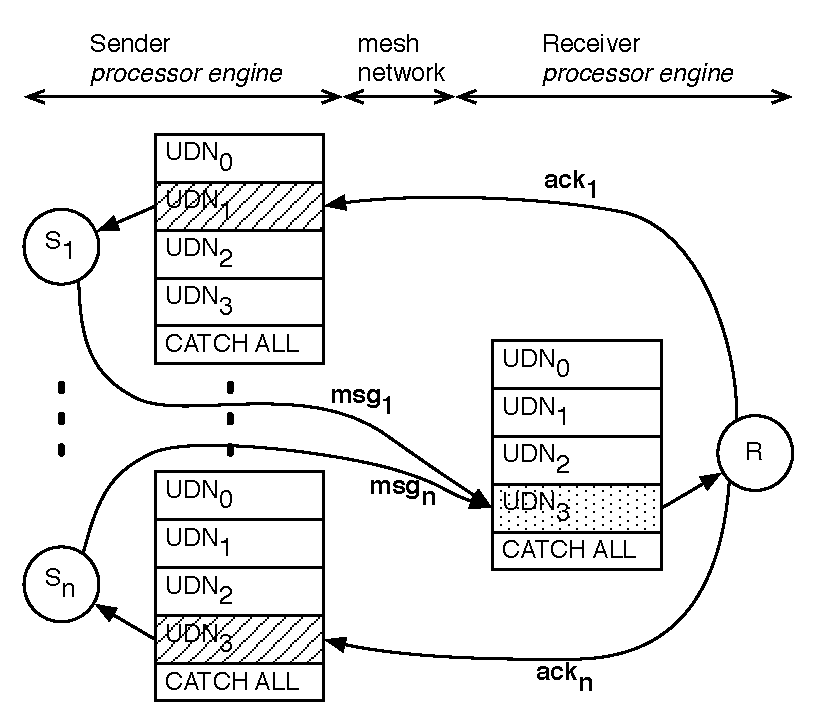
\includegraphics[scale=.5]{udn_asym.pdf}
  \caption[Comunicazione asimmetrica su UDN]{Rappresentazione di un possibile scenario di comunicazione asimmetrica in ingresso tra l'insieme di processi mittenti $\{ S_1, \dots, S_n \}$ e il processo destinatario R, sfruttando la UDN}
  \label{fig:udn_asym}
\end{figure}
L'implementazione della comunicazione asimmetrica in ingresso deriva da quella simmetrica: un generico processo mittente del canale dispone di una coda UDN sulla quale legge gli eventi di Ack, il processo ricevente del canale usa una singola coda UDN sulla quale legge il messaggio di uno qualsiasi tra i processi mittenti. Un messaggio inviato da un mittente \`e costituito da una coppia di valori: una parola di intestazione contenente l'identificatore del mittente all'interno del canale, e una seconda parola contente il valore del messaggio per il quale \`e stato richiesto l'invio. Il fatto che sia trasmesso anche una intestazione al messaggio \`e trasparente all'utente, in quanto l'esecuzione della ricezione nel processo destinatario rende visibile all'utente solo il valore del messaggio. Come mostrato in figura~\ref{fig:udn_asym} diversi mittenti dello stesso canale possono avere come una coda UDN di ricezione qualsiasi, questo crea un problema simile a quello visto nell'implementazione che sfrutta la memoria condivisa nella sezione~\ref{sct:asymin_sm_rdyack}: durante l'esecuzione della primitiva di invio del canale, da parte di un generico mittente, deve essere noto l'identificatore del mittente all'interno del canale stesso, in modo da sapere quale coda UDN usare per l'evento Ack e che valore dare all'intestazione dei messaggi. Anche per questa implementazione del canale asimmetrico si usa un terzo parametro nella primitiva di invio: l'identificatore nel canale del mittente. Il comportamento del protocollo \`e descritto nel codice~\ref{lst:abstr_udn_asym}; come nel canale simmetrico, il supporto fa uso di un descrittore di canale contenente le informazioni sulle cpu e le code UDN usate dai processi comunicanti, nel caso dei processi mittenti tali informazioni sono organizzate in array accedute con l'identificatore del mittente all'interno del canale.
\begin{lstlisting}[
        float=!h,
        morekeywords={dq_snd, dq_rcv, cpu_snd, cpu_rcv}, 
        caption={Descrizione astratta del protocollo di comunicazione Rdy-Ack su UDN per un canale di comunicazione asimmetrico in ingresso},
        label={lst:abstr_udn_asym}
]
send(ch_descr, msg, rank) ::
  leggi una parola dalla UDN Demux Queue 
    ch_descr->dq_snd[rank]
  invia tramite UDN la sequenza di valori <rank, msg> alla
    UDN Demux Queue ch_descr->dq_rcv del PE
    ch_descr->cpu_rcv

receive(ch_descr) ::
  leggi una parola dalla UDN Demux Queue ch_descr->dq_rcv e
    assega il valore alla variablie sender
  leggi una parola dalla UDN Demux Queue ch_descr->dq_rcv e
    assegna il valore alla variablie targa
  invia tramite UDN una parola arbitraria alla UDN Demux
    Queue ch_descr->dq_snd[sender] del PE 
    ch_descr->cpu_snd[sender]
\end{lstlisting}

L'analisi della correttezza della comunicazione \`e simile a quella descritta nell'implementazione simmetrica: \begin{inparaenum}[\itshape a~\upshape)] \item durante l'implementazione del canale devono essere inviati i messaggi di Ack a tutti i mittenti nelle relative code UDN, \item l'utente si fa carico di non usare in un certo processo, eseguito in modo esclusivo in un PE, la stessa coda UDN per pi\`u canali o compiti diversi\end{inparaenum}. Si osserva inoltre che l'unit\`a di routing di UDN \`e il pacchetto \cite{ug101}, quindi l'invio della coppia di parole $<sender_{rank},\;msg>$ da parte di un mittente non viene mai ricevuta intervallata da altre parole nella coda UDN del destinatario se l'invio \`e stato fatto impostando la coppia di parole come payload di un unico pacchetto. Al contrario l'invio di due pacchetti UDN per l'invio della coppia risulta non corretto per l'implementazione descritta.

Si analizza infine la possibilit\`a di situazioni di deadlock causate dall'uso della UDN, che come descritto nella sezione~\ref{sct:intro_arch_udn} \`e soggetta a tale problema. Anche in questo caso l'uso di un paradigma di comunicazione client-server, con un protocollo caratterizzato da grado di asincronia unitario nega il verificarsi di qualsiasi situazione di deadlock (con le ipotesi di correttezza precedenti). Il supporto della comunicazione \`e infatti caratterizzato da un comportamento client-server con interazione domanda-e-risposta, in cui il servente \`e il destinatario e i mittenti sono i clienti. Le richieste dei clienti sono i messaggi inviati dai clienti e le risposte sono i messaggi di ack inviati dal destinatario. In una computazione di questo tipo il deadlock avviene soltanto se i messaggi di risposta del servente riempono la coda di un cliente, ci\`o accade solo quando un cliente invia pi\`u richieste della capacit\`a della coda UDN di memorizzare le risposte \cite{ug205}.

\FloatBarrier
\subsubsection{Comunicazioni con grado di asincronia maggiore di 1}
\label{sct:ad_gt_1_udn}
Le due implementazioni dei canali simmetrici e asimmetrici che sfruttano UDN si prestano ad essere estese ad un grado di asincronia maggiore di uno, \`e infatti sufficiente inviare un numero $m > 1$ di messaggi di Ack al/i mettente/i in fase di inizializzazione del canale. In questo modo eseguendo lo stesso protocollo precedentemente definito si ha un comportamento asincrono di grado $m$. 

Occorre porre attenzione al fatto che un grado di asincronia elevato pu\`o causare il deadlock dell'applicazione. In particolare un mittente non deve inviare pi\`u messaggi della dimensione della coda di demultiplexing UDN. Dato che in entrambe le forme di canale le risposte del destinatario hanno dimensione una parola allora il massimo grado di asincronia \`e la dimensione delle code UDN, per entrambi i canali.

\FloatBarrier
\subsubsection{Implementazione generica}
\label{sct:generic_udn}
Non \`e fornita una implementazione dei canali che sfrutti la UDN e che non limiti per ogni processo il numero di canali utilizzabili. Si descrive qui una possibile implementazione. La limitazione fisica di un numero finito di canali UDN \`e superata utilizzando, con il paradigma precedente, per pi\`u canali ``software'', almeno una coda UDN nel mittente e nel destinatario. I diversi canali ``software'' sono riconosciuti mediante una intestazione ai dati scambiati contenente l'identificatore del canale. \`E necessario ricorrere alla memoria condivisa nel caso in cui il processo destinatario invochi la ricezione su un certo canale e i dati ricevuti dalla coda UDN siano appartenenti ad un altro canale ``software'', perci\`o si memorizzano tali dati per un utilizzo successivo e si continua a testare la coda UDN in attesa dei dati del canale usato. 

Si suppone che una implementazione di questo tipo sia sempre usata insieme all'implementazione ``specializzata su UDN'', pu\`o essere quindi conveniente lasciare le quattro code UDN di demultiplexing a quest'ultima implementazione, e usare la coda \emph{catch all} per l'implementazione ``generica su UDN''. Tale coda viene usata quando si inviano pacchetti UDN con tag di demultiplexing diverso dai quattro valori delle code firmware, la ricezione viene effettuata mediante la lettura di registri SPR. 

L'uso di una implementazione ``UDN generica'' pu\`o essere una utile alternativa alla implementazione che sfrutta esclusivamente la memoria condivisa (descritta in \ref{sct:specifica_sm}) per applicazioni che necessitano di pi\`u di quattro canali per processo e basse latenze di comunicazione. Si osserva tuttavia che pi\`u sono usati molti canali di comunicazione in un singolo processo, pi\`u aumenta la probabilit\`a di ricevere il messaggio di un canale diverso e quindi la necessit\`a di eseguire una copia in memoria (overhead).




\newpage
\section{Esperimenti}
\label{sct:esperimenti}
Con lo scopo di stimare e confrontare le prestazioni delle due tipologie di implementazioni del supporto alle comunicazioni vengono proposti due diversi esperimenti. Il primo \`e volto a misurare la latenza di comunicazione dei canali, viene usato il classico metodo a scambio di messaggi, detto ``ping-pong''. Il secondo \`e la parallelizzazione di un modulo sequenziale su stream che prevede sia comunicazioni simmetriche, che almeno una comunicazione asimmetrica in ingresso; in questo caso il confronto delle due soluzioni si basa sul tempo di completamento dello stream e sulla scalabilit\`a del sistema parallelo all'aumentare del numero dei processi. \`E significativa la scelta del tipo di computazione e di calcolo, in quanto le differenze prestazionali dei supporti forniti emergono con calcoli di grana fine, molto comuni in computazioni su stream. Calcoli di grana elevata, invece, non sono influenzati dalle comunicazioni: se \`e possibile la sovrapposizione delle comunicazioni al calcolo, le comunicazioni non hanno alcun impatto, altrimenti sono trascurabili rispetto al tempo di calcolo.

%% sono realizzati nell'ottica di far fronte a comunicazioni a grana fine. Brevi calcoli aritmetici su stream, ad esempio, risultano problematici nella scalabilit\`a se non si usano comunicazioni efficenti, in particolar modo se non \`e possibile la sovrapposizione delle comunicazioni al calcolo.

\subsection{Misurazione della latenza di comunicazione}
\label{sct:meter}
Si propone un primo confronto delle due tipologie di implementazioni del supporto alle comunicazioni effettuato sulla latenza di comunicazione in \emph{assenza di conflitti} sia sulle reti di interconnessione che sulla memoria condivisa\footnote{Non \`e possibile asserire l'assenza di conflitti in tali sottosistemi, tuttavia, se esistono, i conflitti sono minimi rispetto a quelli che si verificano in una applicazione reale, in quanto l'applicazione di misurazione fa uso di due soli processi che tramite il nostro supporto si sincronizzano a vicenda.}. Per entrambe le forme di comunicazione vogliamo sapere quale \`e il tempo medio necessario ad eseguire completamente una comunicazione, ovvero l'intervallo di tempo medio tra l'inizio dell'esecuzione di una \emph{send} e la copia del messaggio nella variabile targa del destinatario, avvenuta al termine dell'esecuzione della corrispondente \emph{receive} nel destinatario. La latenza di un canale asimmetrico viene misurata con un unico mittente, cos\`i da poter essere confrontata con la latenza di comunicazione di un canale simmetrico. 

Le implementazioni presentate nel Capitolo \ref{sct:specifica_meccanismi} sono riassunte in tabella~\ref{tab:implementazioni} con i rispettivi nomi. 
Una misura di questo tipo \`e una prima risposta al quesito del lavoro di tirocinio: se esistono vantaggi prestazionali nell'uso di UDN per un supporto alle comunicazioni, e che tipo di miglioramenti si hanno rispetto ad una implementazione tradizionale. Questi risultati sono utili anche per un confronto interno alle diverse soluzioni che usano la memoria condivisa e che sono specifiche delle possibilit\`a di configurazione della macchina \tile. La sezione~\ref{sct:specifica_sm} presenta alcune possibili scelte di gestione del sottosistema di memoria cache al fine di minimizzare gli overhead legati alla coerenza. Attraverso questa prima misura siamo quindi interessati a conoscere:
\begin{itemize}
\item quale \`e la degradazione dovuta alla gestione predefinita dell'homing delle strutture dati, senza sfruttare il paradigma consumatore-produttore,
\item quale la degradazione legata all'uso della barriera di memoria necessaria con il protocollo Rdy-Ack e invece eliminata con un diverso protocollo.
\end{itemize}


%% il confronto tra queste e in particolare fornisce una valutazione della degradazione causata da una gestione non ottima della localit\`a in cache o dall'uso dell'istruzione di \emph{memory fence}. Per quanto riguarda il canale asimmetrico su memoria condivisa si \`e implementata solo la versione con protocollo Rdy-Ack e gestione esplicita dell'allocazione in quanto pi\`u generale rispetto alla versione con protocollo Null-Ack che prevede l'uso del valore particolare \verb+NULL+, tuttavia una versione con tale protocollo \`e possibile anche per tale forma di comunicazione. 

%% Nella sezione \ref{sct:specifica_meccanismi} sono stati definiti i meccanismi di comunicazione considerati ed \`e stata fornita la descrizione delle implementazioni degli stessi sfruttando i due supporti architetturali. Per quanto riguarda l'uso di UDN abbiamo una sola implementazione per il canale simmetrico e per il canale asimmetrico che fa uso esclusivo della UDN, questa \`e l'implementazione che fornisce le migliori prestazioni che il supporto architetturale possa offrire. Per quanto riguarda la memoria condivisa invece si sono studiate pi\`u realizzazioni del canale simmetrico per quanto riguarda la massimizzazione della localit\`a delle informazioni del supporto in cache
%% e l'uso di un diverso protocollo di comunicazione che non si serve del blocco di memoria. Per l'implementazione del canale asimmetrico con memoria condivisa si \`e adottata la soluzione pi\`u generica che fa uso del protocollo Rdy-Ack e che alloca esplicitamente il supporto in cache. Le varie implementazioni, con i rispettivi nomi, sono riassunte nella tabella~\ref{tab:implementazioni}.

%% La prima comparazione delle varie realizzazioni viene effettuata sulla latenza di comunicazione in assenza di conflitti sia sulle reti di interconessione che sulla memoria condivisa. Tale tipo di test \`e utile per:

%% \begin{itemize}
%% \item il confronto tra le varie implementazioni con memoria condivisa, in particolare si stabilisce di quanto \`e migliore l'implementazione con gestione esplicita dell'allocazione in cache rispetto a quella predefinita, e che di che entit\`a \`e la degradazione indotta dall'uso dell'istruzione di \emph{memory fence} necessaria nel protocollo Rdy-Ack;
%% \item il confronto tra le implementazioni che fanno uso dei due diversi supporti architetturali, ovvero di quanto \`e ``migliore'' l'implementazione che fa uso di UDN rispetto all'implementazione che fa uso di memoria condivisa.
%% \end{itemize}

\begin{table}[!b]
  \centering
  \begin{tabular}{ |m{15ex}|m{23ex}|m{26ex}| }
    \hline
    \textit{Supporto architetturale} & \textit{Nome dei canali di comunicazione} & \textit{Descrizione} \\
    \hline
    \multirow{5}{15ex}{Memoria Condivisa}  & \verb+ch_sym_sm_rdyack_no+ & Utilizzo non ottimizzato della cache \\
    \cline{2-3}
    & \verb+ch_sym_sm_rdyack+ & \multirow{2}{26ex}{Allocazione con massima localit\`a in cache} \\
    & \verb+ch_asymin_sm+ & \\
%    & \verb+ch_asymin_sm_all+ & \\
    \cline{2-3}
    & \verb+ch_sym_sm_nullack+ & Utilizzo del protocollo di comunicazione Null-Ack \\
    \hline
    \multirow{2}{*}{UDN} & \verb+ch_sym_udn+ & \multirow{2}{26ex}{Uso esclusivo della rete di interconnessione} \\
    & \verb+ch_asymin_udn+ & \\
    \hline
  \end{tabular}
  \caption[Nomi dei canali di comunicazione realizzati]{Canali di comunicazione implementati con i due supporti architetturali}
  \label{tab:implementazioni}
\end{table}

\subsubsection{L'applicazione di misurazione}
Al fine di valutare la latenza di comunicazione (\Lcom) dei canali si misura il tempo di completamento (\Tc) di una applicazione di tipo ``ping-pong'' caratterizzato da due processi comunicanti mediante due canali con direzione una opposta a quella dell'altro. I due canali hanno stessa forma e stessa implementazione. Il comportamento di ciascun processo \`e definito dall'alternarsi di invio di un messaggio e ricezione di un messaggio rispettivamente sui due canali collegati al processo. Il processo che esegue per prima operazione la \emph{send} \`e detto ``white process'', l'altro, che comincia eseguendo \emph{receive}, \`e detto ``black process''. La sequenza temporale delle azioni eseguite dai due processi \`e mostrata in figura~\ref{fig:schema_metering}. Per \Tc\ si intende il tempo impiegato per lo scambio di un numero $n$ di messaggi, tale tempo \`e preso nel white process memorizzando il tempo di avvio, prima del primo invio, e il tempo di fine, dopo l'$n$-esima ricezione. Prima di eseguire gli $n$ scambi i due processi effettuano uno o pi\`u scambi ``non misurati'' affinch\`e l'uso successivo dei canali trovi i blocchi del supporto gi\`a presenti in cache. 

La latenza di comunicazione \`e approssimata come la met\`a del tempo medio di scambio:
\[ \inTscambio = \frac{\inTc}{n} \qquad \inLcom = \frac{\inTscambio}{2} \] \\

\begin{figure}[!t]
  \centering
  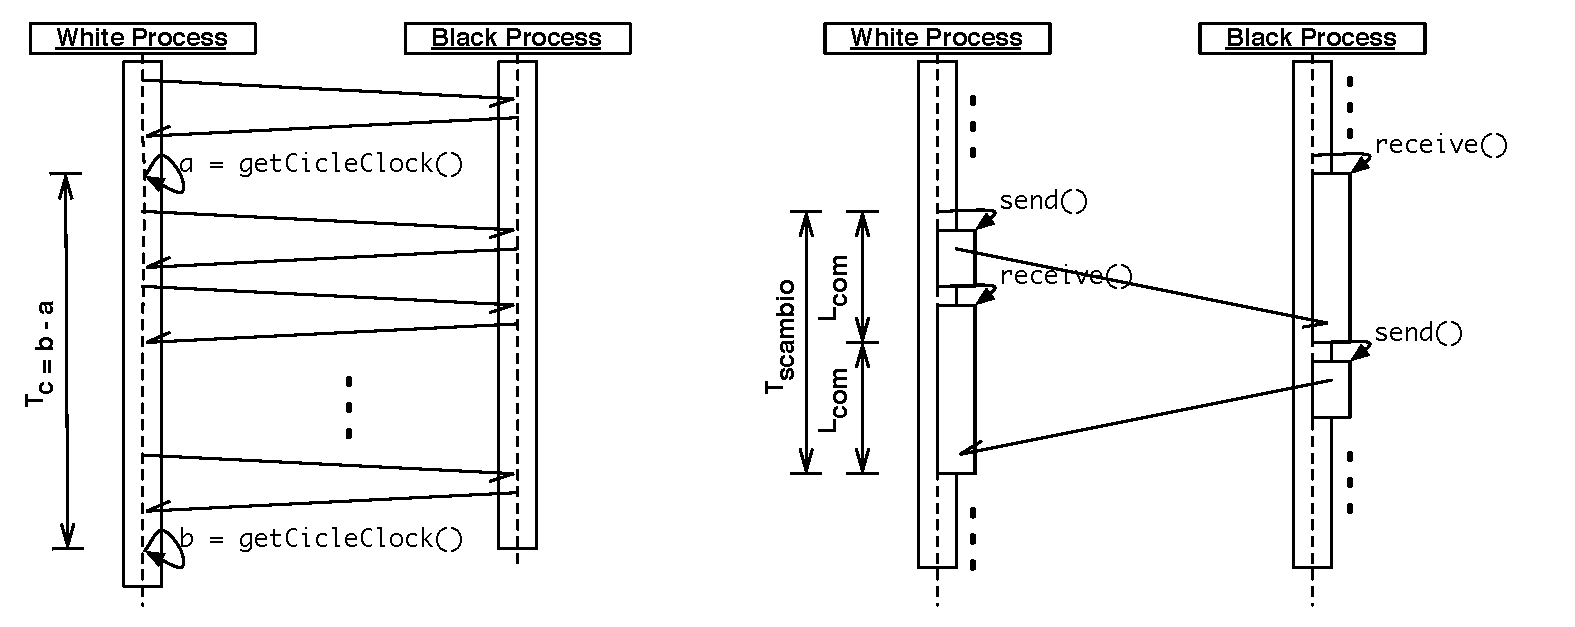
\includegraphics[scale=.5]{schema_metering.pdf}
  \caption[Comportamento temporale dell'applicazione ``ping-pong'']{Rappresentazione della sequenza di azioni svolte dai due processi dell'applicazione di misurazione. A sinistra viene mostrato il comportamento complessivo, a destra il dettaglio di uno scambio di messaggi.}
  \label{fig:schema_metering}
\end{figure}

Il programma di misurazione effettua $m$ scambi di messaggi. L'esecuzione e la corrispondente misurazione del tempo di completamento degli scambi \`e eseguita per diverse configurazioni di allocazione dei processi nei PE, a distanze diverse nella mesh. I valori di distanza, o \emph{numero di hops}, considerati sono: il minimo (1), il massimo (14) e quello medio ($\sqrt{64} = 8$). Per ogni configurazione vengono eseguite $n$ misure, ad ogni iterazione viene calcolato il valore medio della latenza di comunicazione per gli $m$ scambi effettuati. Per ogni distanza viene presentata la media, il valore massimo e la devianza standard degli $n$ valori medi della latenza di comunicazione. 

Nella misurazione della comunicazione asimmetrica si prendono in considerazione solo le due principali implementazioni del supporto, ovvero quella che fa uso della UDN e quella che utilizza al meglio la memoria condivisa \footnote{Per determinare questa informazione si usano i risultati della misura delle implementazioni simmetriche, si veda la discussione nella sezione~\ref{sct:meter_risultati}}. Inoltre, per la stessa forma di comunicazione e per quanto riguarda l'implementazione su memoria condivisa, viene fornita un'altra misura, chiamata \verb+ch_asymin_sm_all+. Viene utilizzato un canale asimmetrico con il massimo numero di processi mittenti allocabili nella macchina; come in precedenza, la misura \`e effettuata con lo scambio di messaggi tra due soli processi. La misura \`e interessante in quanto la politica di ricezione del destinatario prevede la scansione del flag \verb+Rdy+ di tutti i processi mittenti. \`E pertanto auspicabile un aumento della latenza di comunicazione con l'aumento del numero dei mittenti, anche se solo uno di questi comunica con il destinatario. Si osserva che questo secondo modo di misurare la comunicazione asimmetrica non fornisce risultati significati per l'implementazione UDN, e per questo motivo non \`e mostrato nei risultati. Con l'uso di UDN, infatti, la politica di ricezione non deterministica da pi\`u mittenti \`e implementata nativamente dal firmware della macchina e non \`e soggetta a overhead (\`e la lettura da una coda FIFO di registri).


\subsubsection{Risultati}
\label{sct:meter_risultati}
\begin{figure}[p]
  \centering
  \begin{subfigure}[b]{.5\textheight}
    %% $ cd meter_data
    %% $ ./compact 2_4_*.dat
    %% $ ./printAll  2 4
    %% $ ./plot.sh 2 4
    %% $ cd ..
    %% $ cp meter_data/2_4_{sym,asymin}_all.{tex,pdf} ./
    \resizebox{\columnwidth}{!}{% GNUPLOT: LaTeX picture with Postscript
\begingroup
  \makeatletter
  \providecommand\color[2][]{%
    \GenericError{(gnuplot) \space\space\space\@spaces}{%
      Package color not loaded in conjunction with
      terminal option `colourtext'%
    }{See the gnuplot documentation for explanation.%
    }{Either use 'blacktext' in gnuplot or load the package
      color.sty in LaTeX.}%
    \renewcommand\color[2][]{}%
  }%
  \providecommand\includegraphics[2][]{%
    \GenericError{(gnuplot) \space\space\space\@spaces}{%
      Package graphicx or graphics not loaded%
    }{See the gnuplot documentation for explanation.%
    }{The gnuplot epslatex terminal needs graphicx.sty or graphics.sty.}%
    \renewcommand\includegraphics[2][]{}%
  }%
  \providecommand\rotatebox[2]{#2}%
  \@ifundefined{ifGPcolor}{%
    \newif\ifGPcolor
    \GPcolortrue
  }{}%
  \@ifundefined{ifGPblacktext}{%
    \newif\ifGPblacktext
    \GPblacktexttrue
  }{}%
  % define a \g@addto@macro without @ in the name:
  \let\gplgaddtomacro\g@addto@macro
  % define empty templates for all commands taking text:
  \gdef\gplbacktext{}%
  \gdef\gplfronttext{}%
  \makeatother
  \ifGPblacktext
    % no textcolor at all
    \def\colorrgb#1{}%
    \def\colorgray#1{}%
  \else
    % gray or color?
    \ifGPcolor
      \def\colorrgb#1{\color[rgb]{#1}}%
      \def\colorgray#1{\color[gray]{#1}}%
      \expandafter\def\csname LTw\endcsname{\color{white}}%
      \expandafter\def\csname LTb\endcsname{\color{black}}%
      \expandafter\def\csname LTa\endcsname{\color{black}}%
      \expandafter\def\csname LT0\endcsname{\color[rgb]{1,0,0}}%
      \expandafter\def\csname LT1\endcsname{\color[rgb]{0,1,0}}%
      \expandafter\def\csname LT2\endcsname{\color[rgb]{0,0,1}}%
      \expandafter\def\csname LT3\endcsname{\color[rgb]{1,0,1}}%
      \expandafter\def\csname LT4\endcsname{\color[rgb]{0,1,1}}%
      \expandafter\def\csname LT5\endcsname{\color[rgb]{1,1,0}}%
      \expandafter\def\csname LT6\endcsname{\color[rgb]{0,0,0}}%
      \expandafter\def\csname LT7\endcsname{\color[rgb]{1,0.3,0}}%
      \expandafter\def\csname LT8\endcsname{\color[rgb]{0.5,0.5,0.5}}%
    \else
      % gray
      \def\colorrgb#1{\color{black}}%
      \def\colorgray#1{\color[gray]{#1}}%
      \expandafter\def\csname LTw\endcsname{\color{white}}%
      \expandafter\def\csname LTb\endcsname{\color{black}}%
      \expandafter\def\csname LTa\endcsname{\color{black}}%
      \expandafter\def\csname LT0\endcsname{\color{black}}%
      \expandafter\def\csname LT1\endcsname{\color{black}}%
      \expandafter\def\csname LT2\endcsname{\color{black}}%
      \expandafter\def\csname LT3\endcsname{\color{black}}%
      \expandafter\def\csname LT4\endcsname{\color{black}}%
      \expandafter\def\csname LT5\endcsname{\color{black}}%
      \expandafter\def\csname LT6\endcsname{\color{black}}%
      \expandafter\def\csname LT7\endcsname{\color{black}}%
      \expandafter\def\csname LT8\endcsname{\color{black}}%
    \fi
  \fi
  \setlength{\unitlength}{0.0500bp}%
  \begin{picture}(7200.00,5040.00)%
    \gplgaddtomacro\gplbacktext{%
      \csname LTb\endcsname%
      \put(946,704){\makebox(0,0)[r]{\strut{} 0}}%
      \put(946,1128){\makebox(0,0)[r]{\strut{} 50}}%
      \put(946,1553){\makebox(0,0)[r]{\strut{} 100}}%
      \put(946,1977){\makebox(0,0)[r]{\strut{} 150}}%
      \put(946,2402){\makebox(0,0)[r]{\strut{} 200}}%
      \put(946,2826){\makebox(0,0)[r]{\strut{} 250}}%
      \put(946,3251){\makebox(0,0)[r]{\strut{} 300}}%
      \put(946,3675){\makebox(0,0)[r]{\strut{} 350}}%
      \put(2223,484){\makebox(0,0){\strut{}1}}%
      \put(3369,484){\makebox(0,0){\strut{}8}}%
      \put(4514,484){\makebox(0,0){\strut{}14}}%
      \put(5791,704){\makebox(0,0)[l]{\strut{} 0}}%
      \put(5791,1071){\makebox(0,0)[l]{\strut{} 0.05}}%
      \put(5791,1438){\makebox(0,0)[l]{\strut{} 0.1}}%
      \put(5791,1805){\makebox(0,0)[l]{\strut{} 0.15}}%
      \put(5791,2172){\makebox(0,0)[l]{\strut{} 0.2}}%
      \put(5791,2539){\makebox(0,0)[l]{\strut{} 0.25}}%
      \put(5791,2906){\makebox(0,0)[l]{\strut{} 0.3}}%
      \put(5791,3273){\makebox(0,0)[l]{\strut{} 0.35}}%
      \put(5791,3640){\makebox(0,0)[l]{\strut{} 0.4}}%
      \put(176,2189){\rotatebox{-270}{\makebox(0,0){\strut{}$\mathrm{L}_{\mathrm{com}} \; (\,\tau\,)$}}}%
      \put(6692,2189){\rotatebox{-270}{\makebox(0,0){\strut{}$\mathrm{L}_{\mathrm{com}} \; (\,\mu\mathrm{sec}\,)$}}}%
      \put(3368,154){\makebox(0,0){\strut{}number of hops}}%
    }%
    \gplgaddtomacro\gplfronttext{%
      \csname LTb\endcsname%
      \put(4804,4867){\makebox(0,0)[r]{\strut{}\texttt{ch\_sym\_udn}}}%
      \csname LTb\endcsname%
      \put(4804,4647){\makebox(0,0)[r]{\strut{}\texttt{ch\_sym\_sm\_rdyack\_no}}}%
      \csname LTb\endcsname%
      \put(4804,4427){\makebox(0,0)[r]{\strut{}\texttt{ch\_sym\_sm\_rdyack}}}%
      \csname LTb\endcsname%
      \put(4804,4207){\makebox(0,0)[r]{\strut{}\texttt{ch\_sym\_sm\_nullack}}}%
    }%
    \gplbacktext
    \put(0,0){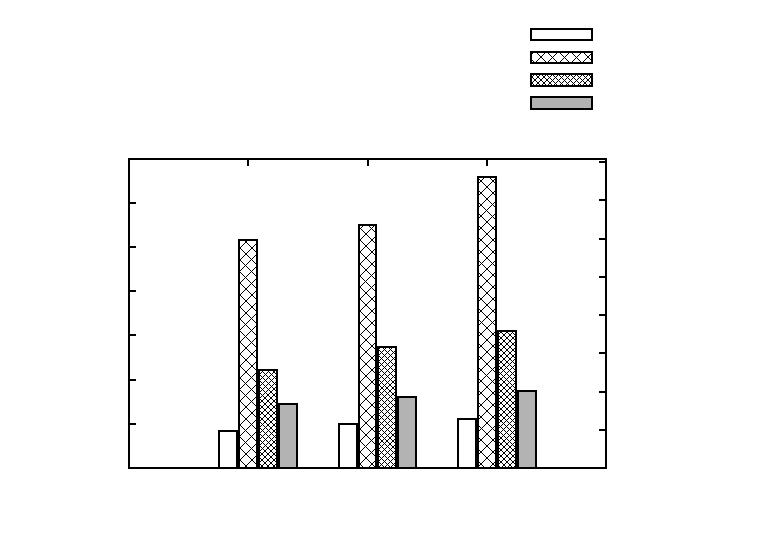
\includegraphics{2_5_sym_all_bw}}%
    \gplfronttext
  \end{picture}%
\endgroup
}
    \caption{Latenza di comunicazione misurata delle implementazioni del canale simmetrico}
    \label{fig:meter_ch_sym_2_4}
  \end{subfigure}
  \\
  \vspace{1cm}
  \begin{subfigure}[b]{.5\textheight}
    \resizebox{\columnwidth}{!}{% GNUPLOT: LaTeX picture with Postscript
\begingroup
  \makeatletter
  \providecommand\color[2][]{%
    \GenericError{(gnuplot) \space\space\space\@spaces}{%
      Package color not loaded in conjunction with
      terminal option `colourtext'%
    }{See the gnuplot documentation for explanation.%
    }{Either use 'blacktext' in gnuplot or load the package
      color.sty in LaTeX.}%
    \renewcommand\color[2][]{}%
  }%
  \providecommand\includegraphics[2][]{%
    \GenericError{(gnuplot) \space\space\space\@spaces}{%
      Package graphicx or graphics not loaded%
    }{See the gnuplot documentation for explanation.%
    }{The gnuplot epslatex terminal needs graphicx.sty or graphics.sty.}%
    \renewcommand\includegraphics[2][]{}%
  }%
  \providecommand\rotatebox[2]{#2}%
  \@ifundefined{ifGPcolor}{%
    \newif\ifGPcolor
    \GPcolortrue
  }{}%
  \@ifundefined{ifGPblacktext}{%
    \newif\ifGPblacktext
    \GPblacktexttrue
  }{}%
  % define a \g@addto@macro without @ in the name:
  \let\gplgaddtomacro\g@addto@macro
  % define empty templates for all commands taking text:
  \gdef\gplbacktext{}%
  \gdef\gplfronttext{}%
  \makeatother
  \ifGPblacktext
    % no textcolor at all
    \def\colorrgb#1{}%
    \def\colorgray#1{}%
  \else
    % gray or color?
    \ifGPcolor
      \def\colorrgb#1{\color[rgb]{#1}}%
      \def\colorgray#1{\color[gray]{#1}}%
      \expandafter\def\csname LTw\endcsname{\color{white}}%
      \expandafter\def\csname LTb\endcsname{\color{black}}%
      \expandafter\def\csname LTa\endcsname{\color{black}}%
      \expandafter\def\csname LT0\endcsname{\color[rgb]{1,0,0}}%
      \expandafter\def\csname LT1\endcsname{\color[rgb]{0,1,0}}%
      \expandafter\def\csname LT2\endcsname{\color[rgb]{0,0,1}}%
      \expandafter\def\csname LT3\endcsname{\color[rgb]{1,0,1}}%
      \expandafter\def\csname LT4\endcsname{\color[rgb]{0,1,1}}%
      \expandafter\def\csname LT5\endcsname{\color[rgb]{1,1,0}}%
      \expandafter\def\csname LT6\endcsname{\color[rgb]{0,0,0}}%
      \expandafter\def\csname LT7\endcsname{\color[rgb]{1,0.3,0}}%
      \expandafter\def\csname LT8\endcsname{\color[rgb]{0.5,0.5,0.5}}%
    \else
      % gray
      \def\colorrgb#1{\color{black}}%
      \def\colorgray#1{\color[gray]{#1}}%
      \expandafter\def\csname LTw\endcsname{\color{white}}%
      \expandafter\def\csname LTb\endcsname{\color{black}}%
      \expandafter\def\csname LTa\endcsname{\color{black}}%
      \expandafter\def\csname LT0\endcsname{\color{black}}%
      \expandafter\def\csname LT1\endcsname{\color{black}}%
      \expandafter\def\csname LT2\endcsname{\color{black}}%
      \expandafter\def\csname LT3\endcsname{\color{black}}%
      \expandafter\def\csname LT4\endcsname{\color{black}}%
      \expandafter\def\csname LT5\endcsname{\color{black}}%
      \expandafter\def\csname LT6\endcsname{\color{black}}%
      \expandafter\def\csname LT7\endcsname{\color{black}}%
      \expandafter\def\csname LT8\endcsname{\color{black}}%
    \fi
  \fi
  \setlength{\unitlength}{0.0500bp}%
  \begin{picture}(7200.00,5040.00)%
    \gplgaddtomacro\gplbacktext{%
      \csname LTb\endcsname%
      \put(946,704){\makebox(0,0)[r]{\strut{} 0}}%
      \put(946,1059){\makebox(0,0)[r]{\strut{} 50}}%
      \put(946,1413){\makebox(0,0)[r]{\strut{} 100}}%
      \put(946,1768){\makebox(0,0)[r]{\strut{} 150}}%
      \put(946,2122){\makebox(0,0)[r]{\strut{} 200}}%
      \put(946,2477){\makebox(0,0)[r]{\strut{} 250}}%
      \put(946,2831){\makebox(0,0)[r]{\strut{} 300}}%
      \put(946,3186){\makebox(0,0)[r]{\strut{} 350}}%
      \put(946,3540){\makebox(0,0)[r]{\strut{} 400}}%
      \put(946,3895){\makebox(0,0)[r]{\strut{} 450}}%
      \put(2256,484){\makebox(0,0){\strut{}1}}%
      \put(3435,484){\makebox(0,0){\strut{}8}}%
      \put(4613,484){\makebox(0,0){\strut{}14}}%
      \put(5923,704){\makebox(0,0)[l]{\strut{} 0}}%
      \put(5923,1317){\makebox(0,0)[l]{\strut{} 0.1}}%
      \put(5923,1930){\makebox(0,0)[l]{\strut{} 0.2}}%
      \put(5923,2543){\makebox(0,0)[l]{\strut{} 0.3}}%
      \put(5923,3156){\makebox(0,0)[l]{\strut{} 0.4}}%
      \put(5923,3769){\makebox(0,0)[l]{\strut{} 0.5}}%
      \put(176,2299){\rotatebox{-270}{\makebox(0,0){\strut{}$\mathrm{L}_{\mathrm{com}} \; (\,\tau\,)$}}}%
      \put(6692,2299){\rotatebox{-270}{\makebox(0,0){\strut{}$\mathrm{L}_{\mathrm{com}} \; (\,\mu\mathrm{sec}\,)$}}}%
      \put(3434,154){\makebox(0,0){\strut{}number of hops}}%
    }%
    \gplgaddtomacro\gplfronttext{%
      \csname LTb\endcsname%
      \put(4936,4867){\makebox(0,0)[r]{\strut{}\texttt{ch\_asymin\_udn}}}%
      \csname LTb\endcsname%
      \put(4936,4647){\makebox(0,0)[r]{\strut{}\texttt{ch\_asymin\_sm\_all}}}%
      \csname LTb\endcsname%
      \put(4936,4427){\makebox(0,0)[r]{\strut{}\texttt{ch\_asymin\_sm}}}%
    }%
    \gplbacktext
    \put(0,0){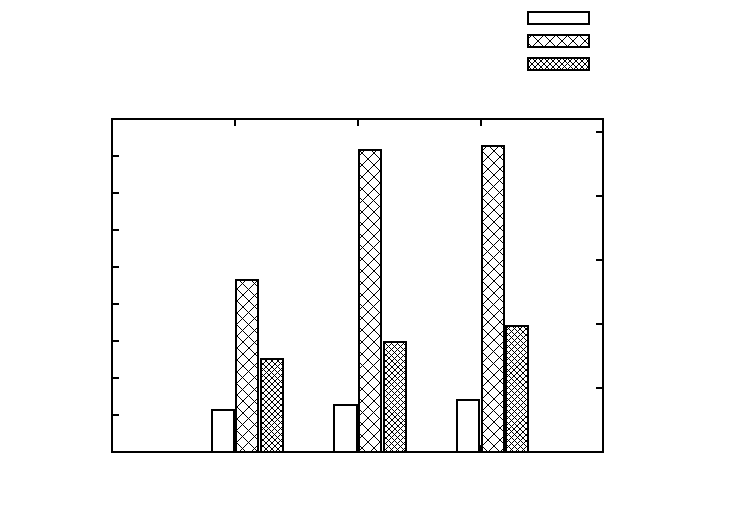
\includegraphics{2_5_asymin_all_bw}}%
    \gplfronttext
  \end{picture}%
\endgroup
}
    \caption{Latenza di comunicazione misurata delle implementazioni del canale asimmetrico in ingresso}
    \label{fig:meter_ch_asymin_2_4}
  \end{subfigure}
  \caption[Latenza di comunicazione dei canali]{Rappresentazione grafica dei risultati delle misurazioni della latenza di comunicazione dei canali. Il programma di misurazione \`e stato eseguito con un numero $m = 10^5$ di scambi e un numero $n = 10$ di iterazioni.}
  \label{fig:meter_type2_nscamb4}
\end{figure}

\begin{table}[!b]
  \centering
  \begin{subtable}[b]{\textwidth}
    \centering
    \begin{tabular}{|l|r|r|r|r|r|}
      \hline
      \multirow{3}{*}{\emph{Implementazione}} &
      \multirow{3}{4ex}{\emph{\# Hops}} &
      \multicolumn{4}{|c|}{$\inLcom$} \\
      \cline{3-6}
      & & \multicolumn{2}{|c|}{\emph{Avg}} &
      \multirow{2}{*}{\emph{Std Dev}} &
      \multirow{2}{*}{\emph{Max} $(\,\tau\,)$} \\
      \cline{3-4}
      & & $\tau$ & $\mu\mathrm{sec}$ & & \\
      \hline
      %% \multirow{3}{18ex}{\texttt{ch\_sym\_udn}} 
      %% & 1 & 42.066550 & 0.048655 & 0.097822 & 42.262000 \\
      %% & 8 & 49.561120 & 0.057323 & 0.104196 & 49.769500 \\
      %% & 14 & 55.722760 & 0.064450 & 0.107943 & 55.792050 \\
      %% \hline
      %% \multirow{3}{18ex}{\texttt{ch\_sym\_sm\_rdyack\_no}} 
      %% & 1 & 257.800490 & 0.298178 & 0.008955 & 257.815900 \\
      %% & 8 & 275.320380 & 0.318442 & 0.006685 & 275.327650 \\
      %% & 14 & 329.332180 & 0.380914 & 0.018220 & 329.363400 \\
      %% \hline
      %% \multirow{3}{18ex}{\texttt{ch\_sym\_rdyack\_sm}}
      %% & 1 & 111.482450 & 0.128943 & 0.187050 & 111.653200 \\
      %% & 8 & 137.378440 & 0.158895 & 0.016294 & 137.395550 \\
      %% & 14 & 155.377520 & 0.179713 & 0.013281 & 155.393950 \\
      %% \hline
      %% \multirow{3}{18ex}{\texttt{ch\_sym\_sm\_nullack}}
      %% & 1 & 72.359500 & 0.083692 & 0.219423 & 72.549500 \\ 
      %% & 8 & 80.700840 & 0.093340 & 0.124463 & 80.827350 \\ 
      %% & 14 & 86.759230 & 0.100347 & 0.118203 & 86.826250 \\
      \multirow{3}{*}{\texttt{ch\_sym\_udn}} 
      & 1 & 42.067 & 0.04866 & 0.09782 & 42.262 \\
      & 8 & 49.561 & 0.05732 & 0.10419 & 49.770 \\
      & 14 & 55.723 & 0.06445 & 0.10794 & 55.792 \\
      \hline
      \multirow{3}{*}{\texttt{ch\_sym\_sm\_rdyack\_no}} 
      & 1 & 257.800 & 0.29818 & 0.00896 & 257.816 \\
      & 8 & 275.320 & 0.31844 & 0.00669 & 275.328 \\
      & 14 & 329.332 & 0.38091 & 0.01822 & 329.363 \\
      \hline
      \multirow{3}{*}{\texttt{ch\_sym\_rdyack\_sm}}
      & 1 & 111.482 & 0.12894 & 0.18701 & 111.653 \\
      & 8 & 137.378 & 0.15890 & 0.01633 & 137.396 \\
      & 14 & 155.378 & 0.17971 & 0.01328 & 155.394 \\
      \hline
      \multirow{3}{*}{\texttt{ch\_sym\_sm\_nullack}}
      & 1 & 72.360 & 0.08369 & 0.21942 & 72.550 \\ 
      & 8 & 80.701 & 0.09334 & 0.12446 & 80.827 \\ 
      & 14 & 86.759 & 0.10034 & 0.11820 & 86.826 \\
      \hline
    \end{tabular}
    \caption[Latenza dei canali di comunicazione simmetrici]{Misurazione della latenza di comunicazione simmetrica delle diverse implementazioni.}
  \end{subtable}

  %%%%%%%%%%%%%%%%%%%%%%%%%%%%%%%%%%%%%%%%%%%%%%%%%%%%%%%%%%%%%%%%%%%%%%%%%%%%%%%%
  \vspace{4ex}
  %%%%%%%%%%%%%%%%%%%%%%%%%%%%%%%%%%%%%%%%%%%%%%%%%%%%%%%%%%%%%%%%%%%%%%%%%%%%%%%%

  \begin{subtable}[b]{\textwidth}
    \centering
    \begin{tabular}{|l|r|r|r|r|r|}
      \hline
      \multirow{3}{*}{\emph{Implementazione}} &
      \multirow{3}{4ex}{\emph{\# Hops}} &
      \multicolumn{4}{|c|}{$\inLcom$} \\
      \cline{3-6}
      & & \multicolumn{2}{|c|}{\emph{Avg}} &
      \multirow{2}{*}{\emph{Std Dev}} &
      \multirow{2}{*}{\emph{Max} $(\,\tau\,)$} \\
      \cline{3-4}
      & & $\tau$ & $\mu\mathrm{sec}$ & & \\
      \hline
      %% \multirow{3}{*}{\texttt{ch\_asymin\_udn}}
      %% & 1 & 56.025529 & 0.064800 & 0.000941 & 56.026905 \\
      %% & 8 & 63.525349 & 0.073475 & 0.000979 & 63.526575 \\
      %% & 14 & 69.527121 & 0.080416 & 0.001011 & 69.528720 \\
      %% \hline
      %% \multirow{3}{*}{\texttt{ch\_asymin\_sm\_all}}
      %% & 1 & 230.570268 & 0.266683 & 0.028743 & 230.643940 \\
      %% & 8 & 408.779285 & 0.472804 & 0.047859 & 408.846645 \\
      %% & 14 & 414.374837 & 0.479276 & 0.025326 & 414.417200 \\
      %% \hline
      %% \multirow{3}{*}{\texttt{ch\_asymin\_sm}}
      %% & 1 & 125.039207 & 0.144623 & 0.001632 & 125.041220 \\
      %% & 8 & 149.041103 & 0.172384 & 0.001936 & 149.045050 \\
      %% & 14 & 170.037299 & 0.196669 & 0.002036 & 170.040285 \\
      \multirow{3}{*}{\texttt{ch\_asymin\_udn}}
      & 1 & 56.0255 & 0.06480 & 0.00094 & 56.027 \\
      & 8 & 63.525 & 0.07348 & 0.00098 & 63.527 \\
      & 14 & 69.527 & 0.08042 & 0.00101 & 69.529 \\
      \hline
      \multirow{3}{*}{\texttt{ch\_asymin\_sm\_all}}
      & 1 & 230.570 & 0.26668 & 0.02874 & 230.644 \\
      & 8 & 408.779 & 0.47280 & 0.04786 & 408.847 \\
      & 14 & 414.375 & 0.47928 & 0.02533 & 414.417 \\
      \hline
      \multirow{3}{*}{\texttt{ch\_asymin\_sm}}
      & 1 & 125.039 & 0.14462 & 0.00163 & 125.041 \\
      & 8 & 149.041 & 0.17238 & 0.00194 & 149.045 \\
      & 14 & 170.037 & 0.19667 & 0.00204 & 170.040 \\
      \hline
    \end{tabular}
    \caption{Misurazione della latenza di comunicazione asimmetrica in ingresso delle diverse implementazioni.}
  \end{subtable}

  \caption[Latenza dei canali di comunicazione asimmetrici]{Misure della latenza di comunicazione rilevate iterando 10 volte il programma ``ping-pong'' con $m = 10^5$ scambi }
  \label{tab:meter}
\end{table}

I risultati proposti in tabella~\ref{tab:meter} e graficamente in figura~\ref{fig:meter_type2_nscamb4}, sono relativi a 10 iterazioni del programma di misurazione con $m = 10^5$ scambi di messaggi tra i due processi.

I risultati ottenuti verificano i ragionamenti descritti nelle Sezioni \ref{sct:specifica_sm}, \ref{sct:specifica_udn} che hanno guidato la realizzazione delle diverse implementazioni. La prima considerazione riguarda il confronto tra l'uso della UDN e della memoria condivisa: in entrambe le forme di comunicazione l'implementazione di UDN ha latenza inferiore a quella dell'implementazione con memoria condivisa pi\`u veloce. Raffiniamo questa osservazione valutando quale sia la migliore implementazione su memoria condivisa e quindi confrontiamola con l'implementazione UDN. La migliore implementazione su SM non \`e necessariamente quella pi\`u veloce: sebbene il protocollo Null-Ack fornisca la minor latenza, la sua implementazione fa uso di un valore particolare dei messaggi e pertanto \`e meno generica delle altre implementazioni. Ad esempio se si richiedesse una implementazione di canali di tipo generico, l'applicazione di questo protocollo potrebbe essere problematica. L'implementazione Null-Ack \`e utile per conoscere quale \`e la degradazione introdotta dalla barriera di memoria, necessaria nel protocollo Rdy-Ack, e quindi quale \`e il vero overhead della nostra implementazione lock-free dei canali. 

Passiamo a valutare la differenza tra le due implementazioni su SM che usano il protocollo Rdy-Ack e che differiscono per la gestione della gerarchia cache. Una gestione esplicita dell'allocazione in cache, che massimizzi la localit\`a dei dati, dimezza la latenza di comunicazione rispetto alla gestione predefinita dell'allocazione. Questo \`e un risultato generale, l'impostazione del PE consumatore come Home per il dato acceduto in computazioni \emph{consumatore~-~produttore} risulta determinante per ottimizzare le prestazioni; considerazioni simili sono state valutate in contesti differenti \cite{buono2013parallel}. Consideriamo quindi la \verb+ch_sym_sm_rdyack+ come implementazione candidata su memoria condivisa, che usa il protocollo Rdy-Ack. Osserviamo che il rapporto tra la latenza di questa soluzione e quella con il protocollo Null-Ack (sempre su SM) \`e di 1.68. Dato che le due implementazioni eseguono istruzioni simili, con la solo differenza della barriera di memoria, \`e ragionevole valutare la causa di questo aumento della latenza come l'esecuzione della memory fence.\\
Si osserva inoltre che l'implementazione Rdy-Ack \`e leggermente pi\`u sensibile alla variazione di distanza dei due processi, rispetto alla Null-Ack; quest'ultima ha un aumento della latenza pari a tanti cicli di clock quanto \`e l'aumento della distanza. Si nota che in questo aspetto la Null-Ack si comporta come la UDN. 
%%La seconda osservazione sulle implementazioni SM riguarda la gestione esplicita della gerarchia cache al fine di massimizzare la localit\`a dei dati: questa possibilit\`a risulta essere fondamentale per le prestazioni su memoria condivisa. L'uso della gestione predefinita \`e due volte pi\`u lento della versione con il descrittore di canale partizionato e homed nelle caches consumatori. \\
%%Si considera \verb+ch_sym_sm_rdyack+ l'implementazione migliore su SM. 

Si considera infine il rapporto tra la soluzione su SM e quella su UDN. Il vantaggio di uso dell'implementazione UDN rispetto a quella SM \`e significativo: mediamente la latenza UDN \`e inferiore pi\`u della met\`a (1/2.737) di quella SM. 

Il confronto dei canali asimmetrici con un singolo mittente ha risultato simile al confronto precedente. In questo caso il rapporto medio tra la latenze UDN e quella SM, 1/2.341, \`e leggermente maggiore. \`E significativo anche il confronto tra questi canali e i corrispondenti simmetrici, in quanto, nel programma di misurazione, i canali asimmetrici sono utilizzati per realizzare forme di comunicazione simmetrica. In entrambi i casi si ha un aumento della latenza di circa 10 cicli di clock. Ci\`o pu\`o essere spiegato dalle specifiche implementazioni parallele: con l'uso della UDN il mittente invia due parole, anzich\`e una del caso simmetrico; con l'uso della SM abbiamo l'uso di altre variabili, ad esempio per garantire la fairness, rispetto al caso simmetrico. \\
Si osserva infine che esiste una differenza sostanziale tra l'uso del canale asimmetrico su SM con un singolo mittente rispetto a quello con tutti i mittenti, ma uno solo attivo. La latenza nel secondo caso \`e mediamente il doppio di quella con un singolo mittente, ne segue un divario ancora pi\`u ampio con la latenza del canale su UDN.\\



%% media dei rapporti tra rdyack e nullack 1.678
%% media dei rapporti tra rdyack_no e rdy ack 2.145
%% media dei rapporti tra udn e rdyack 2.737
%% media dei rapporti tra asym_udn e asym_sm 2.341
%% media dei rapporti tra asym_udn e asym_sm_all 5.503





%% \begin{figure}[!h]
%%   \centering
%%   \resizebox{\columnwidth}{!}{% GNUPLOT: LaTeX picture with Postscript
\begingroup
  \makeatletter
  \providecommand\color[2][]{%
    \GenericError{(gnuplot) \space\space\space\@spaces}{%
      Package color not loaded in conjunction with
      terminal option `colourtext'%
    }{See the gnuplot documentation for explanation.%
    }{Either use 'blacktext' in gnuplot or load the package
      color.sty in LaTeX.}%
    \renewcommand\color[2][]{}%
  }%
  \providecommand\includegraphics[2][]{%
    \GenericError{(gnuplot) \space\space\space\@spaces}{%
      Package graphicx or graphics not loaded%
    }{See the gnuplot documentation for explanation.%
    }{The gnuplot epslatex terminal needs graphicx.sty or graphics.sty.}%
    \renewcommand\includegraphics[2][]{}%
  }%
  \providecommand\rotatebox[2]{#2}%
  \@ifundefined{ifGPcolor}{%
    \newif\ifGPcolor
    \GPcolortrue
  }{}%
  \@ifundefined{ifGPblacktext}{%
    \newif\ifGPblacktext
    \GPblacktexttrue
  }{}%
  % define a \g@addto@macro without @ in the name:
  \let\gplgaddtomacro\g@addto@macro
  % define empty templates for all commands taking text:
  \gdef\gplbacktext{}%
  \gdef\gplfronttext{}%
  \makeatother
  \ifGPblacktext
    % no textcolor at all
    \def\colorrgb#1{}%
    \def\colorgray#1{}%
  \else
    % gray or color?
    \ifGPcolor
      \def\colorrgb#1{\color[rgb]{#1}}%
      \def\colorgray#1{\color[gray]{#1}}%
      \expandafter\def\csname LTw\endcsname{\color{white}}%
      \expandafter\def\csname LTb\endcsname{\color{black}}%
      \expandafter\def\csname LTa\endcsname{\color{black}}%
      \expandafter\def\csname LT0\endcsname{\color[rgb]{1,0,0}}%
      \expandafter\def\csname LT1\endcsname{\color[rgb]{0,1,0}}%
      \expandafter\def\csname LT2\endcsname{\color[rgb]{0,0,1}}%
      \expandafter\def\csname LT3\endcsname{\color[rgb]{1,0,1}}%
      \expandafter\def\csname LT4\endcsname{\color[rgb]{0,1,1}}%
      \expandafter\def\csname LT5\endcsname{\color[rgb]{1,1,0}}%
      \expandafter\def\csname LT6\endcsname{\color[rgb]{0,0,0}}%
      \expandafter\def\csname LT7\endcsname{\color[rgb]{1,0.3,0}}%
      \expandafter\def\csname LT8\endcsname{\color[rgb]{0.5,0.5,0.5}}%
    \else
      % gray
      \def\colorrgb#1{\color{black}}%
      \def\colorgray#1{\color[gray]{#1}}%
      \expandafter\def\csname LTw\endcsname{\color{white}}%
      \expandafter\def\csname LTb\endcsname{\color{black}}%
      \expandafter\def\csname LTa\endcsname{\color{black}}%
      \expandafter\def\csname LT0\endcsname{\color{black}}%
      \expandafter\def\csname LT1\endcsname{\color{black}}%
      \expandafter\def\csname LT2\endcsname{\color{black}}%
      \expandafter\def\csname LT3\endcsname{\color{black}}%
      \expandafter\def\csname LT4\endcsname{\color{black}}%
      \expandafter\def\csname LT5\endcsname{\color{black}}%
      \expandafter\def\csname LT6\endcsname{\color{black}}%
      \expandafter\def\csname LT7\endcsname{\color{black}}%
      \expandafter\def\csname LT8\endcsname{\color{black}}%
    \fi
  \fi
  \setlength{\unitlength}{0.0500bp}%
  \begin{picture}(7200.00,5040.00)%
    \gplgaddtomacro\gplbacktext{%
      \csname LTb\endcsname%
      \put(946,704){\makebox(0,0)[r]{\strut{} 0}}%
      \put(946,1128){\makebox(0,0)[r]{\strut{} 50}}%
      \put(946,1553){\makebox(0,0)[r]{\strut{} 100}}%
      \put(946,1977){\makebox(0,0)[r]{\strut{} 150}}%
      \put(946,2402){\makebox(0,0)[r]{\strut{} 200}}%
      \put(946,2826){\makebox(0,0)[r]{\strut{} 250}}%
      \put(946,3251){\makebox(0,0)[r]{\strut{} 300}}%
      \put(946,3675){\makebox(0,0)[r]{\strut{} 350}}%
      \put(2223,484){\makebox(0,0){\strut{}1}}%
      \put(3369,484){\makebox(0,0){\strut{}8}}%
      \put(4514,484){\makebox(0,0){\strut{}14}}%
      \put(5791,704){\makebox(0,0)[l]{\strut{} 0}}%
      \put(5791,1071){\makebox(0,0)[l]{\strut{} 0.05}}%
      \put(5791,1438){\makebox(0,0)[l]{\strut{} 0.1}}%
      \put(5791,1805){\makebox(0,0)[l]{\strut{} 0.15}}%
      \put(5791,2172){\makebox(0,0)[l]{\strut{} 0.2}}%
      \put(5791,2539){\makebox(0,0)[l]{\strut{} 0.25}}%
      \put(5791,2906){\makebox(0,0)[l]{\strut{} 0.3}}%
      \put(5791,3273){\makebox(0,0)[l]{\strut{} 0.35}}%
      \put(5791,3640){\makebox(0,0)[l]{\strut{} 0.4}}%
      \put(176,2189){\rotatebox{-270}{\makebox(0,0){\strut{}$\mathrm{L}_{\mathrm{com}} \; (\,\tau\,)$}}}%
      \put(6692,2189){\rotatebox{-270}{\makebox(0,0){\strut{}$\mathrm{L}_{\mathrm{com}} \; (\,\mu\mathrm{sec}\,)$}}}%
      \put(3368,154){\makebox(0,0){\strut{}number of hops}}%
    }%
    \gplgaddtomacro\gplfronttext{%
      \csname LTb\endcsname%
      \put(4261,4867){\makebox(0,0)[r]{\strut{}\texttt{ch\_sym\_udn}}}%
      \csname LTb\endcsname%
      \put(4261,4647){\makebox(0,0)[r]{\strut{}\texttt{ch\_sym\_sm\_rdyack\_no}}}%
      \csname LTb\endcsname%
      \put(4261,4427){\makebox(0,0)[r]{\strut{}\texttt{ch\_sym\_sm\_rdyack}}}%
      \csname LTb\endcsname%
      \put(4261,4207){\makebox(0,0)[r]{\strut{}\texttt{ch\_sym\_sm\_nullack}}}%
    }%
    \gplbacktext
    \put(0,0){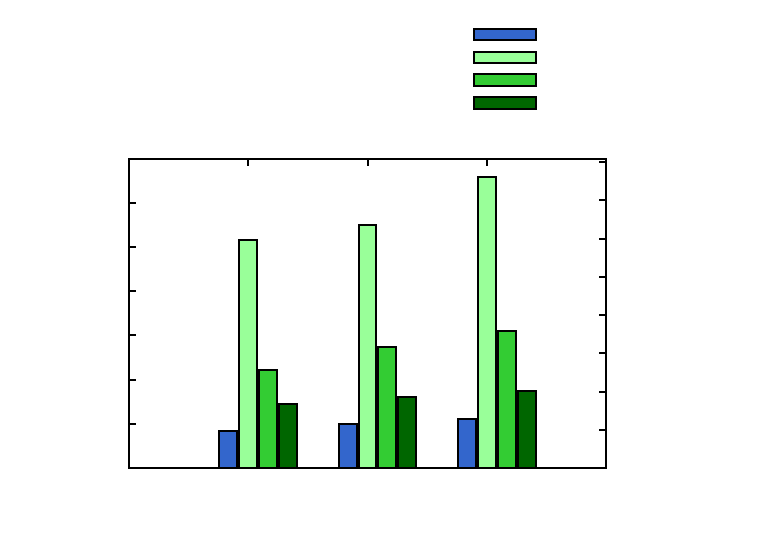
\includegraphics{2_5_sym_all}}%
    \gplfronttext
  \end{picture}%
\endgroup
}
%%   \caption{}
%%   \label{fig:meter_ch_sym_2_5}
%% \end{figure}

%% \begin{figure}[!hb]
%%   \centering
%%   \resizebox{\columnwidth}{!}{% GNUPLOT: LaTeX picture with Postscript
\begingroup
  \makeatletter
  \providecommand\color[2][]{%
    \GenericError{(gnuplot) \space\space\space\@spaces}{%
      Package color not loaded in conjunction with
      terminal option `colourtext'%
    }{See the gnuplot documentation for explanation.%
    }{Either use 'blacktext' in gnuplot or load the package
      color.sty in LaTeX.}%
    \renewcommand\color[2][]{}%
  }%
  \providecommand\includegraphics[2][]{%
    \GenericError{(gnuplot) \space\space\space\@spaces}{%
      Package graphicx or graphics not loaded%
    }{See the gnuplot documentation for explanation.%
    }{The gnuplot epslatex terminal needs graphicx.sty or graphics.sty.}%
    \renewcommand\includegraphics[2][]{}%
  }%
  \providecommand\rotatebox[2]{#2}%
  \@ifundefined{ifGPcolor}{%
    \newif\ifGPcolor
    \GPcolortrue
  }{}%
  \@ifundefined{ifGPblacktext}{%
    \newif\ifGPblacktext
    \GPblacktexttrue
  }{}%
  % define a \g@addto@macro without @ in the name:
  \let\gplgaddtomacro\g@addto@macro
  % define empty templates for all commands taking text:
  \gdef\gplbacktext{}%
  \gdef\gplfronttext{}%
  \makeatother
  \ifGPblacktext
    % no textcolor at all
    \def\colorrgb#1{}%
    \def\colorgray#1{}%
  \else
    % gray or color?
    \ifGPcolor
      \def\colorrgb#1{\color[rgb]{#1}}%
      \def\colorgray#1{\color[gray]{#1}}%
      \expandafter\def\csname LTw\endcsname{\color{white}}%
      \expandafter\def\csname LTb\endcsname{\color{black}}%
      \expandafter\def\csname LTa\endcsname{\color{black}}%
      \expandafter\def\csname LT0\endcsname{\color[rgb]{1,0,0}}%
      \expandafter\def\csname LT1\endcsname{\color[rgb]{0,1,0}}%
      \expandafter\def\csname LT2\endcsname{\color[rgb]{0,0,1}}%
      \expandafter\def\csname LT3\endcsname{\color[rgb]{1,0,1}}%
      \expandafter\def\csname LT4\endcsname{\color[rgb]{0,1,1}}%
      \expandafter\def\csname LT5\endcsname{\color[rgb]{1,1,0}}%
      \expandafter\def\csname LT6\endcsname{\color[rgb]{0,0,0}}%
      \expandafter\def\csname LT7\endcsname{\color[rgb]{1,0.3,0}}%
      \expandafter\def\csname LT8\endcsname{\color[rgb]{0.5,0.5,0.5}}%
    \else
      % gray
      \def\colorrgb#1{\color{black}}%
      \def\colorgray#1{\color[gray]{#1}}%
      \expandafter\def\csname LTw\endcsname{\color{white}}%
      \expandafter\def\csname LTb\endcsname{\color{black}}%
      \expandafter\def\csname LTa\endcsname{\color{black}}%
      \expandafter\def\csname LT0\endcsname{\color{black}}%
      \expandafter\def\csname LT1\endcsname{\color{black}}%
      \expandafter\def\csname LT2\endcsname{\color{black}}%
      \expandafter\def\csname LT3\endcsname{\color{black}}%
      \expandafter\def\csname LT4\endcsname{\color{black}}%
      \expandafter\def\csname LT5\endcsname{\color{black}}%
      \expandafter\def\csname LT6\endcsname{\color{black}}%
      \expandafter\def\csname LT7\endcsname{\color{black}}%
      \expandafter\def\csname LT8\endcsname{\color{black}}%
    \fi
  \fi
  \setlength{\unitlength}{0.0500bp}%
  \begin{picture}(7200.00,5040.00)%
    \gplgaddtomacro\gplbacktext{%
      \csname LTb\endcsname%
      \put(946,704){\makebox(0,0)[r]{\strut{} 0}}%
      \put(946,1059){\makebox(0,0)[r]{\strut{} 50}}%
      \put(946,1413){\makebox(0,0)[r]{\strut{} 100}}%
      \put(946,1768){\makebox(0,0)[r]{\strut{} 150}}%
      \put(946,2122){\makebox(0,0)[r]{\strut{} 200}}%
      \put(946,2477){\makebox(0,0)[r]{\strut{} 250}}%
      \put(946,2831){\makebox(0,0)[r]{\strut{} 300}}%
      \put(946,3186){\makebox(0,0)[r]{\strut{} 350}}%
      \put(946,3540){\makebox(0,0)[r]{\strut{} 400}}%
      \put(946,3895){\makebox(0,0)[r]{\strut{} 450}}%
      \put(2256,484){\makebox(0,0){\strut{}1}}%
      \put(3435,484){\makebox(0,0){\strut{}8}}%
      \put(4613,484){\makebox(0,0){\strut{}14}}%
      \put(5923,704){\makebox(0,0)[l]{\strut{} 0}}%
      \put(5923,1317){\makebox(0,0)[l]{\strut{} 0.1}}%
      \put(5923,1930){\makebox(0,0)[l]{\strut{} 0.2}}%
      \put(5923,2543){\makebox(0,0)[l]{\strut{} 0.3}}%
      \put(5923,3156){\makebox(0,0)[l]{\strut{} 0.4}}%
      \put(5923,3769){\makebox(0,0)[l]{\strut{} 0.5}}%
      \put(176,2299){\rotatebox{-270}{\makebox(0,0){\strut{}$\mathrm{L}_{\mathrm{com}} \; (\,\tau\,)$}}}%
      \put(6692,2299){\rotatebox{-270}{\makebox(0,0){\strut{}$\mathrm{L}_{\mathrm{com}} \; (\,\mu\mathrm{sec}\,)$}}}%
      \put(3434,154){\makebox(0,0){\strut{}number of hops}}%
    }%
    \gplgaddtomacro\gplfronttext{%
      \csname LTb\endcsname%
      \put(4129,4867){\makebox(0,0)[r]{\strut{}\texttt{ch\_asymin\_udn}}}%
      \csname LTb\endcsname%
      \put(4129,4647){\makebox(0,0)[r]{\strut{}\texttt{ch\_asymin\_sm\_all}}}%
      \csname LTb\endcsname%
      \put(4129,4427){\makebox(0,0)[r]{\strut{}\texttt{ch\_asymin\_sm}}}%
    }%
    \gplbacktext
    \put(0,0){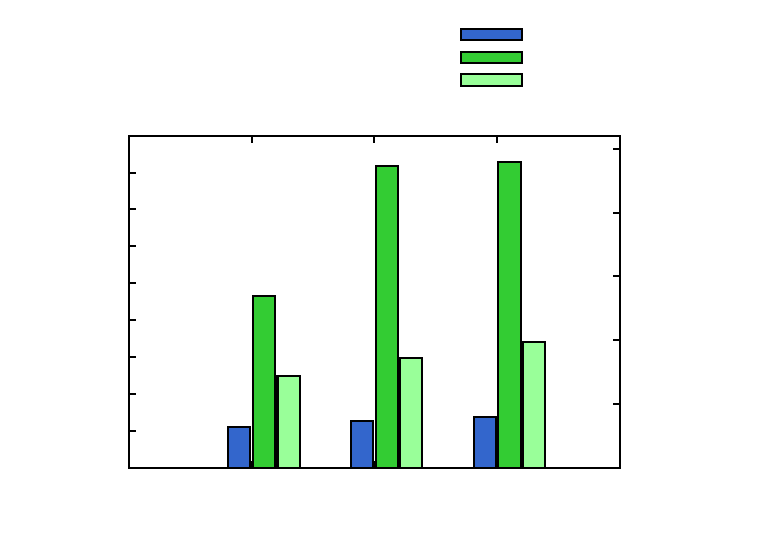
\includegraphics{2_5_asymin_all}}%
    \gplfronttext
  \end{picture}%
\endgroup
}
%%   \caption{}
%%   \label{fig:meter_ch_asymin_2_5}
%% \end{figure}


%%%%%%%%%%%%%%%%%%%%%%%%%%%%%%%%%%%%%%%%%%%%%%%%%%%%%%%%%%%%%%%%%%%%%%%%%%%%%%%%


  
\FloatBarrier


%% \begin{table}[!h]
%%   \centering
%%   \begin{tabular}{|l|l|l|l|l|}
%%     \hline
%%     \multirow{2}{22ex}{\emph{Implemenatation}} & \multirow{2}{*}{\emph{\#Hops}} & \multicolumn{3}{|c|}{$\inLcom \; (\tau)$} \\
%%     \cline{3-5}
%%     & & \emph{Avg} & \emph{Std Dev} & \emph{Max} \\
%%     \hline
%%     \multirow{3}{18ex}{\texttt{ch\_asymin\_udn}} & \\
%%     & \\
%%     & \\
%%     \hline
%%     \multirow{3}{18ex}{\texttt{ch\_asymin\_sm\_no}} & \\
%%     & \\
%%     & \\
%%     \hline
%%     \multirow{3}{18ex}{\texttt{ch\_asymin\_sm}} & \\
%%     & \\
%%     & \\
%%     \hline
%%   \end{tabular}
%%   \caption{Risultati numerici, in cicli di clock, della misurazione della latenza di comunicazione asimmetrica in ingresso delle diverse implementazioni.}
%% \end{table}



%% \begin{table}[!h]
%%   \centering
%%   \begin{subtable}[b]{\textwidth}
%%     \begin{tabular}{|l|l|l|l|l|}
%%       \hline
%%       \multirow{2}{22ex}{\emph{Implemenatation}} & \multirow{2}{*}{\emph{\#Hops}} & \multicolumn{3}{|c|}{$\inLcom \; (\tau)$} \\
%%       \cline{3-5}
%%       & & \emph{Avg} & \emph{Std Dev} & \emph{Max} \\
%%       \hline
%%       \multirow{3}{18ex}{\texttt{ch\_sym\_udn}} & 1 & 42.066550 & 0.097822 & 42.262000 \\
%%       & 8 & 49.561120 & 0.104196 & 49.769500 \\
%%       & 14 & 55.722760 & 0.107943 & 55.792050 \\
%%       \hline
%%       \multirow{3}{18ex}{\texttt{ch\_sym\_sm\_no}} & 1 & 257.800490 & 0.008955 & 257.815900 \\
%%       & 8 & 275.320380 & 0.006685 & 275.327650 \\
%%       & 14 & 329.332180 & 0.018220 & 329.363400 \\
%%       \hline
%%       \multirow{3}{18ex}{\texttt{ch\_sym\_sm}} & 1 & 111.482450 & 0.187050 & 111.653200 \\
%%       & 8 & 137.378440 & 0.016294 & 137.395550 \\
%%       & 14 & 155.377520 & 0.013281 & 155.393950 \\
%%       \hline
%%       \multirow{3}{18ex}{\texttt{ch\_sym\_sm\_nullack}} & 1 & 72.359500 & 0.219423 & 72.549500 \\ 
%%       & 8 & 80.700840 & 0.124463 & 80.827350 \\ 
%%       & 14 & 86.759230 & 0.118203 & 86.826250 \\
%%       \hline
%%     \end{tabular}
%%     \caption{Misurazione della latenza di comunicazione simmetrica delle diverse implementazioni.}
%%   \end{subtable}

%%   %%%%%%%%%%%%%%%%%%%%%%%%%%%%%%%%%%%%%%%%%%%%%%%%%%%%%%%%%%%%%%%%%%%%%%%%%%%%%%%%
%%   \vspace{4ex}
%%   %%%%%%%%%%%%%%%%%%%%%%%%%%%%%%%%%%%%%%%%%%%%%%%%%%%%%%%%%%%%%%%%%%%%%%%%%%%%%%%%

%%   \begin{subtable}[b]{\textwidth}
%%     \centering
%%     \begin{tabular}{|l|l|l|l|l|}
%%       \hline
%%       \multirow{2}{22ex}{\emph{Implemenatation}} & \multirow{2}{*}{\emph{\#Hops}} & \multicolumn{3}{|c|}{$\inLcom \; (\tau)$} \\
%%       \cline{3-5}
%%       & & \emph{Avg} & \emph{Std Dev} & \emph{Max} \\
%%       \hline
%%       \multirow{3}{18ex}{\texttt{ch\_asymin\_udn}} & 1 & 56.025529 & 0.000941 & 56.026905 \\
%%       & 8 & 63.525349 & 0.000979 & 63.526575 \\
%%       & 14 & 69.527121 & 0.001011 & 69.528720 \\
%%       \hline
%%       \multirow{3}{18ex}{\texttt{ch\_asymin\_sm\_all}} & 1 & 230.570268 & 0.028743 & 230.643940 \\
%%       & 8 & 408.779285 & 0.047859 & 408.846645 \\
%%       & 14 & 414.374837 & 0.025326 & 414.417200 \\
%%       \hline
%%       \multirow{3}{18ex}{\texttt{ch\_asymin\_sm}} & 1 & 125.039207 & 0.001632 & 125.041220 \\
%%       & 8 & 149.041103 & 0.001936 & 149.045050 \\
%%       & 14 & 170.037299 & 0.002036 & 170.040285 \\
%%       \hline
%%     \end{tabular}
%%     \caption{Misurazione della latenza di comunicazione asimmetrica in ingresso delle diverse implementazioni.}
%%   \end{subtable}

%%   \caption{Misure della latenza di comunicazione rilevate iterando 10 volte il programma ``ping-pong'' con $m = 10^5$ scambi }

%% \end{table}




\null
\vfill
\newpage

\subsection{Benchmark moltiplicazione matrice-vettore}
In questa sezione viene proposto un secondo esperimento volto a verificare il comportamento delle implementazioni del supporto su SM e su UDN in una applicazione realistica, con un numero di processi parametrico e potenzialmente alto (fino al massimo numero di PE disponibili, visto l'uso del mapping esclusivo). In particolare \`e stata scelta una applicazione sintetizzata per mezzo di paradigmi di parallelismo che faccia uso sia di comunicazioni simmetriche e di almeno una comunicazione asimmetrica in ingresso. Per mostrare le differenze prestazionali delle due implementazioni la computazione scelta ha calcoli di grana fine e prevede l'elaborazione di dati su stream. Per lo stesso programma sono state eseguite due versioni che utilizzano rispettivamente: solo il supporto alle comunicazioni su SM, e solo il supporto alle comunicazioni su UDN. La principale metrica per il confronto di queste due esecuzioni \`e il tempo di completamento della computazione al variare della dimensione dei dati e del numero di processi usati.

\subsubsection{Descrizione del problema}
Il benchmark proposto si basa su un calcolo numerico di algebra lineare molto frequente nella risoluzione di problemi reali, non solo in ambito scientifico: il prodotto matrice per vettore. Sia $\mathbf{A} = (a_{ij})_{i=1,\ldots,\mathrm{M}, j=1,\ldots,\mathrm{M}} \in \mathbb{Z}^{\mathrm{MxM}}$ una matrice di interi di dimensione MxM, e sia $\mathbf{b} = (b_1,\ldots,b_\mathrm{M}) \in \mathbb{Z}^{\mathrm{M}}$ un vettore di M interi, il risultato dell'operazione prodotto matrice per vettore \`e un vettore $\mathbf{c} = (c_1,\ldots,c_\mathrm{M}) = \mathbf{A} \cdot \mathbf{b} \in \mathbb{Z^{M}}$ la cui componente $i$-esima \`e il prodotto scalare tra la riga $i$-esima di $\mathbf{A}$ e il vettore $\mathbf{b}$.
\[ \forall \; i \in \{1,\ldots,\mathrm{M}\} \; : \; c_i = \mathbf{a}_i \cdot \mathbf{b} = \sum_{j=1}^{\mathrm{M}} a_{ij} \cdot b_j  \]
Dove $\mathbf{a}_i = (a_{i1},\ldots,a_{i\mathrm{M}})$ \`e la riga $i$-esima della matrice $\mathbf{A}$. Da questa definizione segue direttamente l'algoritmo sequenziale del calcolo, che \`e descritto dal codice~\ref{lst:benchmark_seq_alg}.\\
\begin{lstlisting}[float = b, morekeywords = {to}, caption = {Algoritmo sequenziale del calcolo matrice per vettore}, label={lst:benchmark_seq_alg}]
int A[M][M], b[M], c[M];
for i:=0 to M-1 do 
  c[i] := 0;
  for j:=0 to M-1 do
    c[i] := A[i][j]*b[j] + c[i];
\end{lstlisting}

\begin{figure}[!tb]
  \centering
  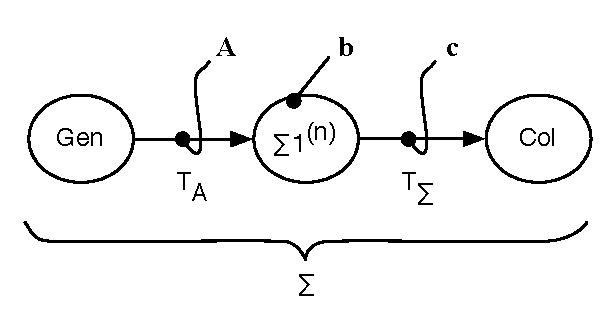
\includegraphics[scale=.5]{grafo_sigma_compatto.pdf}
  \caption[Computazione sequenziale del benchmark]{Rappresentazione compatta del grafo della computazione. L'elemento $\Sigma1$ \`e un modulo sequenziale o un sottosistema parallelo che esegue la moltiplicazione per $\mathbf{b}$ su ogni elemento della matrice. }
  \label{fig:sigma_compatto}
\end{figure}
La computazione considerata riguarda un sistema $\Sigma$ modellato come un grafo aciclico contenente un modulo di elaborazione collegato a due stream, uno di ingresso e l'altro di uscita. Lo stream di ingresso \`e composto da $m$ matrici di interi di dimensione fissata MxM e con un tempo medio di interarrivo \Ta, lo stream di uscita invece trasporta i risultati del calcolo eseguito dal modulo. Su ogni elemento dello stream il modulo calcola la moltiplicazione matrice per vettore utilizzando l'elemento stesso come primo operando e un vettore $\mathbf{b}$, costante per tutta la durata dell'applicazione, come secondo operando. Il vettore risultato di ogni operazione viene scritto nello stream di uscita. 
Ci poniamo nel caso in cui il tempo di calcolo di una moltiplicazione matrice per vettore, \Tcalc, sia superiore al tempo di interarrivo \Ta. Dato che il tempo di servizio della computazione $\Sigma$ \`e  superiore a quello ideale (il tempo di interarrivo dello stream \footnote{Per una trattazione formale della valutazione delle prestazioni di computazioni su stream in grafi aciclici si consulti \cite{hpc_part1}}), si richiede una trasformazione del modulo sequenziale in un sottosistema parallelo funzionalmente equivalente che permetta di eliminare o ridurre il collo di bottiglia nel sistema, determinato dal modulo stesso, e mantenga massima l'efficienza del sottosistema. 
Si indica con \subsystem\ il sottosistema parallelo di calcolo, con grado di parallelismo $n$. 
Dal punto di vista teorico e indipendentemente dalla soluzione parallela scelta, si ha che il tempo di servizio \emph{ideale} del sottosistema parallelo \`e il rapporto tra tempo di calcolo del programma sequenziale e il grado di parallelismo (equazione \ref{eq:TsubsysId}). Il tempo di servizio effettivo del sottosistema \`e invece il massimo valore tra il tempo medio di interarrivo dello stream e il tempo di servizio ideale del sottosistema (equazione \ref{eq:Tsubsys}). Si definisce \emph{efficienza} del sottosistema il rapporto tra i tempi di servizio ideale ed effettivo (equazione \ref{eq:subsysEff}). Ne segue che il sottosistema ha efficienza massima 
%% quando il collo di bottiglia non \`e eliminato dal sottositema, 
se e solo se nella computazione rimane il collo di bottiglia, 
ovvero il grado di parallelismo \emph{non} \`e sufficientemente alto affinch\`e il tempo di servizio ideale sia minore o uguale del tempo di interarrivo. 
Altrimenti, se il collo di bottiglia \`e stato eliminato, l'efficienza non \`e massima e il suo valore corrisponde al \emph{fattore di utilizzazione} del sottosistema, ovvero il rapporto tra il tempo di servizio ideale del sottosistema e il tempo di interarrivo. Da tale caratterizzazione ne segue il valore ottimo del grado di parallelismo, ovvero quel valore di $n$ che consente di eliminare il collo di bottiglia e mantenere massima l'efficienza del sottosistema (equazione \ref{eq:nopt}).
\begin{flalign}
  \label{eq:TsubsysId}
  \inTsubsystemId &= \inTs = \frac{\inTcalc}{n} \\
  \label{eq:Tsubsys}
  \inTsubsystem &= \max(\{\inTa, \; \inTs \}) \\
  \label{eq:subsysEff}
  \inEffic &= \frac{\inTsubsystemId}{\inTsubsystem} = \left\{ \begin{array}{ll} \frac{\inTs}{\inTa}, & \inTs < \inTa \\ 1, & \inTs \ge \inTa \end{array} \right. \in (0,\ldots,1] \\
  \label{eq:nopt}
  n_{\mathrm{opt}} \; &= \; \min(\{ n \in \mathbb{N} \;\, | \;\, \inTs \le \inTa \}) \; = \; \left\lceil \frac{\inTcalc}{\inTa} \right\rceil
\end{flalign}
\\

Altre definizioni utili per caratterizzare le prestazioni dell'applicazione sono le seguenti:
\begin{description}
\item [Tempo di completamento dello stream] \`e definita come il tempo medio impiegato per completare l'esecuzione del calcolo su tutti gli elementi dello stream. Se la lunghezza dello stream $m$ \`e molto superiore al grado di parallelismo $n$ \`e possibile approssimarlo come m volte il tempo medio di servizio del sistema
\begin{equation}
\label{eq:Tc}
m >> n \quad \Rightarrow \quad \inTc = m \cdot \inTsystem
\end{equation}
\item [Scalabilit\`a] esprime il risparmio relativo del tempo medio di servizio che pu\`o essere ottenuto usando l'implementazione parallela con $n$ processi rispetto all'implementazione sequenziale. Pu\`o essere espressa anche in termini del tempo di completamento.
\begin{flalign}
\label{eq:s}
s^{(n)} &= \frac{\inTcalc}{\inTsystem} \\
\label{eq:sId}
s_{\mathrm{id}}^{\phantom{id}(n)} &= \frac{\inTcalc}{\inTsystemId} = \frac{\inTcalc}{\frac{\inTcalc}{n}} = n
\end{flalign}  
%% The speedup of a parallel implementation expresses the relative saving of execution time that can be obtained by using a parallel execution on p processors compared to the best sequential implementation.

\end{description}

\subsubsection{Sul problema scelto}
\begin{figure}[!t]
  \begin{subfigure}[b]{.5\textwidth}
    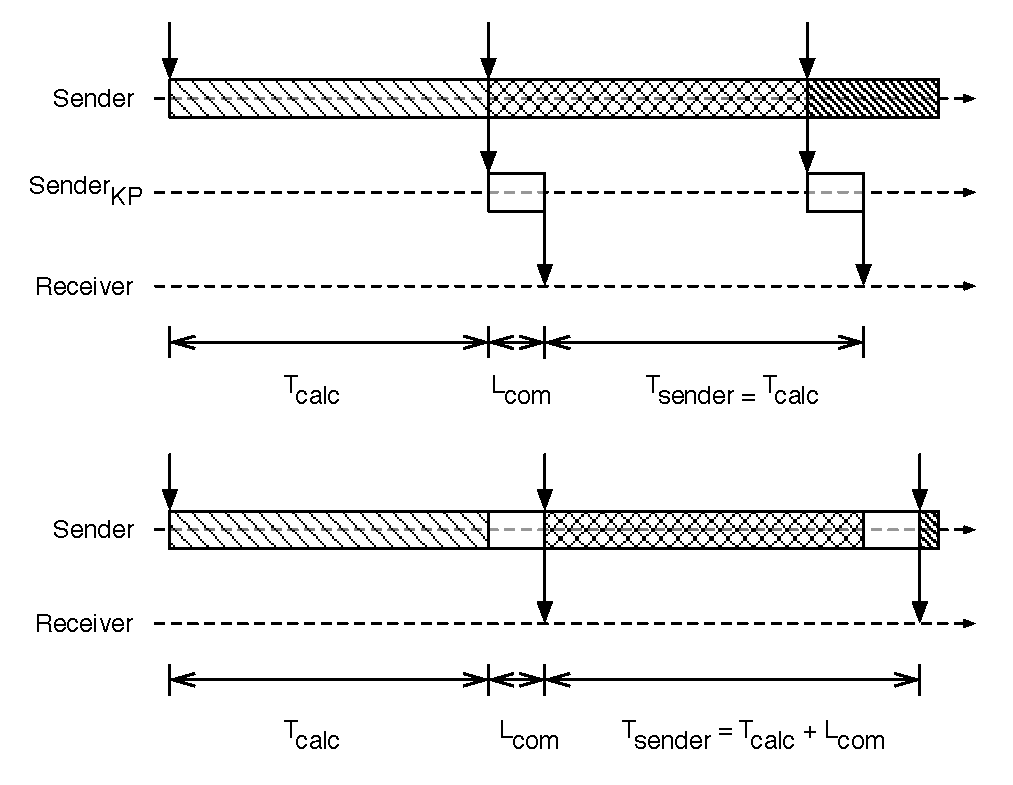
\includegraphics[scale=.38]{servicetime_eg_coarse-grain.pdf}
    \caption{Calcolo di grana grossa}
    \label{fig:eg_coarse_grain}
  \end{subfigure}
  ~
  \begin{subfigure}[b]{.5\textwidth}
    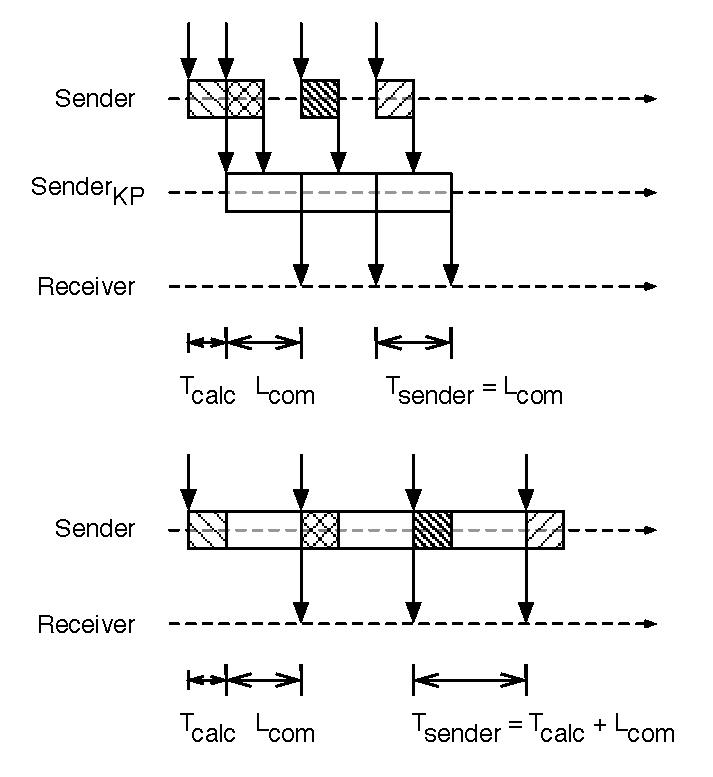
\includegraphics[scale=.38]{servicetime_eg_fine-grain.pdf}
    \caption{Calcolo di grana fine}
    \label{fig:eg_fine_grain}
  \end{subfigure}
  \caption[Esempio di due computazioni su stream con diversa grana]{Rappresentazione grafica di due computazioni con diversa ``grana'' di calcolo, in presenza e in assenza di un processore di comunicazione}
  \label{fig:eg_grain}
\end{figure}
\`E importante soffermarci e motivare il tipo di applicazione scelta: il supporto alle comunicazioni fornito \`e specifico per un dominio applicativo caratterizzato da grana di calcolo fine, se non finissima. Solo in computazioni di questo tipo siamo interessati a ridurre la latenza di comunicazione, e si osservano quindi delle differenze nelle prestazioni globali dell'applicazione. A scopo esemplificativo si considera una parte di una applicazione su stream riguardante due moduli collegati in pipeline: si assume che il tempo di calcolo del primo modulo sia opportunamente dimensionato come il tempo di interarrivo dello stream. Le figure~\ref{fig:eg_coarse_grain},~\ref{fig:eg_fine_grain} mostrano due situazioni con diversa grana di calcolo del primo modulo. Se il tempo di calcolo \`e di diversi ordini di grandezza superiore alla latenza di comunicazione, l'ottimizzazione di qualche centinaio di cicli di clock della comunicazione non consegue alcun vantaggio sul tempo di servizio effettivo del modulo; la comunicazione avr\`a sempre impatto nullo o trascurabile nel tempo di servizio effettivo del modulo. Se \`e possibile la sovrapposizione del calcolo infatti la latenza di comunicazione \`e completamente mascherata dal tempo di calcolo, altrimenti, la latenza di comunicazione si va a sommare al tempo di calcolo, risultando trascurabile. L'ottimizzazione delle comunicazioni \`e invece apprezzabile quando la latenza di queste \`e dello stesso ordine di grandezza del tempo di calcolo. 

Computazioni di grana fine sono molto frequenti nel dominio delle applicazioni su stream di elementi, si pensi a forme di deep packet inspection nel campo della computer networking, nelle quali vengono esaminati specifiche parti di pacchetti, che passano da un punto di ispezione di una rete di computer, alla ricerca di non conformit\`a, o per collezionare statistiche sulle informazioni trasmesse. Computazioni su dato singolo, in special modo quelle che seguono il paradigma Data Parallel sono caratterizzate da grana fine delle computazioni, in seguito al partizionamento del dato. Anche in queste applicazioni \`e utile disporre di un supporto efficiente alle comunicazioni, sia per le forme di comunicazione collettiva, che per le comunicazioni tra moduli in caso di dipendenze sui dati (forme Stencil).

Il Benchmark \`e stato scelto nell'ottica di apprezzare le differenze tra le due realizzazioni del supporto e di verificare il loro comportamento in una applicazione reale. Le due implementazioni del supporto non differiscono solo dal conseguimento di una diversa latenza di comunicazione, come mostrato nell'esperimento precedente. La versione UDN permette un disaccoppiamento tra la comunicazione dei processi e l'accesso ai dati in memoria. La comunicazione tra due processi \`e realizzata interamente con l'uso della UDN e senza l'impiego della memoria condivisa. Ci\`o ha come effetto un numero di richieste alla memoria condivisa minore rispetto all'implementazione dei canali con la memoria. Ci aspettiamo che questo fatto abbia ripercussioni positive sulle prestazioni globali dell'applicazione, non solo per quanto riguarda le comunicazioni, ma in pi\`u in generale, relativamente al tempo di risposta delle richieste alla memoria.
  

\subsubsection{Il metodo di parallelizzazione scelto}
La parallelizzazione del modulo sequenziale \`e stata scelta tra un insieme ristretto (per il tipo di computazione) di paradigmi la cui semantica e modello dei costi sono noti \cite{hpc_part1}, tra cui:
\begin{description}
\item [Farm] \`e caratterizzata dalla replicazione della funzione di calcolo sequenziale in $n$ identiche unit\`a di elaborazione (sottoinsieme delle unit\`a worker). \`E applicabile solo a computazioni su stream, viene usata una unit\`a emettitore per la distribuzione di un elemento dello stream ad un worker, e una unit\`a collettore, collegata ad ogni worker, per ricevere i risultati;
\item [Data Parallel] sono forme di parallelismo che richiedono una discreta conoscenza del calcolo sequenziale ma che per questo motivo risultano flessibili alla specifica computazione. Si basano sul partizionamento dei dati e sulla replicazione della funzione di calcolo nelle unit\`a worker, possono essere applicate sia a singoli dati che a stream di dati; in quest'ultimo caso il partizionamento \`e applicato ad ogni elemento dello stream. I gradi di libert\`a forniti riguardano la strategia di partizionamento dei dati, l'eventuale replicazione di dati, l'organizzazione delle unit\`a worker (indipendenti o interagenti) e il collezionamento dei risultati parziali. Vengono usate forme di comunicazione collettiva per distribuire le partizioni del dato (\emph{scatter}), per collezionare i risultati parziali (\emph{gather}) e/o per costruire il risultato (ad esempio l'operazione di \emph{reduce}). A seconda dell'organizzazione dei workers si distinguono due famiglie di forme Data Parallel: \emph{Map} se ogni worker esegue un calcolo completamente indipendente da quello degli altri worker, \emph{Stencil-based} se esiste un'interazione tra i workers durante l'esecuzione del calcolo.
\end{description}
Si \`e deciso di adottare un paradigma di tipo Data Parallel cos\`i da poter applicare il supporto alle comunicazioni per la realizzazione delle comunicazioni collettive coinvolte, in modo da confrontare le prestazioni dei due tipi di supporto forniti anche relativamente all'implementazione di tali comunicazioni. In particolare, il collezionamento dei risultati sar\`a realizzato per mezzo di un canale asimmetrico in ingresso che ha come mittenti l'insieme dei processi worker dell'implementazione Data Parallel, e come destinatario un processo collettore. Come spiegato in seguito si rende necessaria una distribuzione di ciascun elemento dello stream ai processi worker, piuttosto che una distribuzione delle partizioni di ogni elemento. L'implementazione di questa operazione fa uso dei canali simmetrici ed \`e caratterizzata da una struttura ad albero mappata sull'insieme dei worker. \\

Analizzando le dipendenze sui dati del programma sequenziale (codice~\ref{lst:benchmark_seq_alg}) si osserva che una qualsiasi istruzione di una certa iterazione del ciclo esterno \`e indipendente da tutte le istruzioni di un'altra qualsiasi iterazione dello stesso ciclo. Al contrario ogni istruzione di una iterazione del ciclo interno dipende (\emph{Read-After-Write}) dall'istruzione precedente della stessa iterazione.
\begin{lstlisting}[caption={Rappresentazione delle istruzioni di due cicli esterni contigui.}]
...
{ c[i]:=0; c[i]:=A[i][0]*b[0]+c[i]; c[i]:=A[i][1]*b[1]+c[i]; ... c[i]:=A[i][M-1]*b[M-1]+c[i]; }
{ c[i+1]:=0; c[i+1]:=A[i+1][0]*b[0]+c[i+1]; ... c[i+1]:=A[i+1][M-1]*b[M-1]+c[i+1]; }
...
\end{lstlisting}
Ne segue che pu\`o essere esplicitato del parallelismo sul ciclo esterno, eseguendo iterazioni diverse del ciclo esterno in processi diversi, ottenendo in tal modo un grado massimo di parallelismo $n = \textrm{M}$ e una complessit\`a di esecuzione $O(n)$ contro $O(n^2)$ del calcolo sequenziale. Da ci\`o deriva direttamente il partizionamento delle matrici, che \`e per righe. In tale situazione si ha la ``grana'' minima sia per quanto riguarda le partizioni dei dati, che per il tempo di calcolo.
In generale, un'implementazione effettiva fa uso di un grado di parallelismo $n$ minore di M, dipendentemente dal valore medio del tempo di interarrivo dello stream. In tale situazione le matrici sono sempre partizionate per riga, con grana $g = \lceil M / n \rceil$ righe, il calcolo dei processi worker consiste di $g$ prodotti scalari tra ogni riga della partizione associata al worker e il vettore $\mathbf{b}$. 

Si adotta la replicazione del vettore $\mathbf{b}$ nei processi worker, ci\`o \`e possibile in quanto tale oggetto viene acceduto in sola lettura. Di conseguenza l'implementazione Data Parallel descritta \`e di tipo \emph{Map}. \\

Rispetto a quanto detto finora il sottosistema Map \`e caratterizzato da una comunicazione di \emph{multicast} piuttosto che dalla scatter; infatti si utilizza il supporto alle comunicazioni descritto nella sezione~\ref{sct:specifica_meccanismi} per realizzare gli archi del grafo,
%% \marginpar{RENDERE MEGLIO}
 conseguentemente abbiamo il sottografo Map operante su uno stream di riferimenti. Lo stream di ingresso trasporter\`a i riferimenti alle matrici, la distribuzione di un elemento dello stream ai moduli della Map \`e quindi l'invio dello stesso riferimento agli $n$ moduli; sar\`a poi dovere di ogni worker eseguire il calcolo sulla propria partizione dell'oggetto riferito dal puntatore ricevuto in ingresso. \\

L'implementazione pi\`u semplice della distribuzione multicast fa uso di un singolo processo distributore che in modo sequenziale esegue l'invio del dato ad ogni processo worker. Questa soluzione \`e critica per comunicazioni di grana fine, in quanto pu\`o diventare rapidamente un collo di bottiglia all'aumentare del grado di parallelismo. Considerato l'ambito di applicazioni in si pone il supporto \`e lecito aspettarsi stream caratterizzati da elevata banda, quindi la necessit\`a di disporre di comunicazioni collettive (tra cui la multicast) efficienti, che non siano collo di bottiglia per l'applicazione. Implementazioni della multicast adeguate a questo contesto hanno tempo di servizio costante, ad esempio implementano il processo distributore come un sottosistema parallelo strutturato ad albero. In questo caso, grazie all'effetto-pipeline, il tempo di servizio \`e pari alla latenza di comunicazione di un canale simmetrico per l'ariet\`a dell'albero. Ci\`o richiedere tuttavia nodi aggiuntivi a quelli del sottosistema parallelo. Una soluzione alternativa che mantenga lo stesso tempo di servizio senza moduli addizionali consiste nell'implementare l'albero in modo distribuito direttamente nell'insieme dei moduli worker.
\begin{figure}[!t]
  \centering
  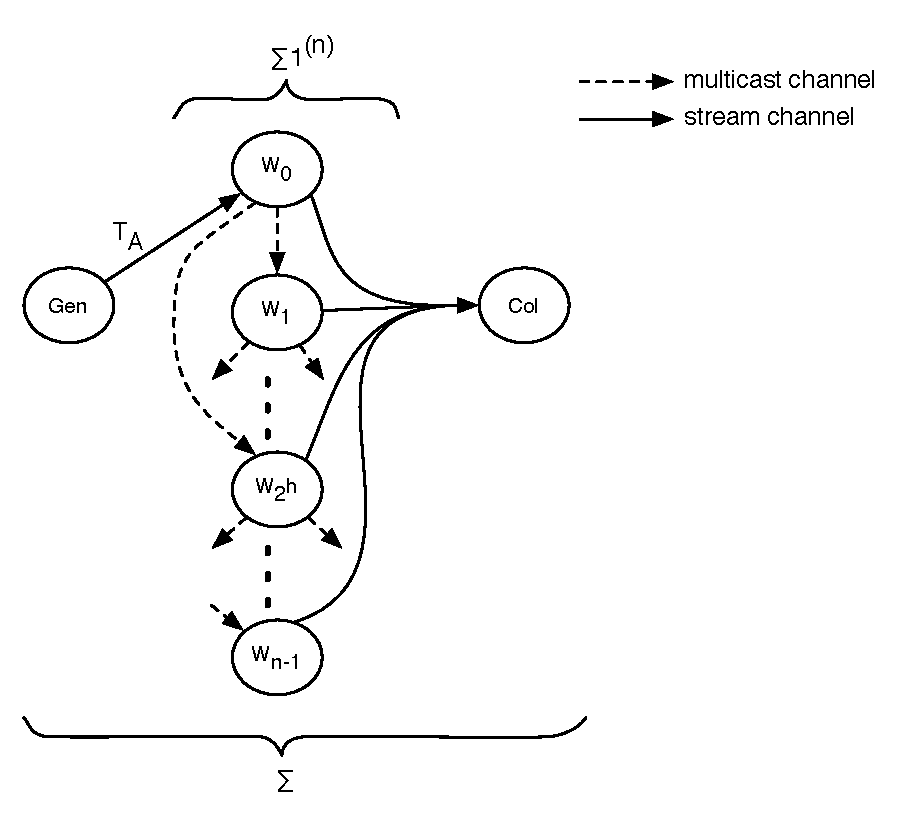
\includegraphics[scale=.5]{grafo_sigma.pdf}
  \caption[Computazione dell'implementazione parallela del benchmark]{Grafo della computazione Map (\subsystem) che \`e collegata allo stream e che fa uso della multicast strutturata ad albero binario mappato sull'insieme di processi worker}
  \label{fig:grafo_map}
\end{figure}
In questo modo, un worker, prima di avviare il proprio calcolo su un elemento dello stream prende parte alla comunicazione multicast dell'elemento stesso realizzata in modo distribuito sull'insieme dei worker. Questa soluzione (per un tempo di interarrivo superiore a 2 volte il tempo di servizio della multicast) permette di risparmiare nodi di elaborazione rispetto ad una soluzione con un sottosistema di nodi specializzato nella distribuzione multicast. 
Di contro, una realizzazione di questo tipo fa pagare il proprio tempo di servizio all'interno del tempo del sottosistema di calcolo nel caso in cui non sia possibile sovrapporre le comunicazioni al calcolo, come accade in \tile\ che non dispone dei supporti architetturali necessari nei PEs per l'esecuzione delle comunicazioni\footnote{Una forma di sovrapposizione esiste quando si fa uso del supporto alle comunicazioni che usa UDN, \`e infatti possibile che il trasferimento del messaggio sia eseguito in modo parzialmente sovrapposto all'esecuzione del calcolo del mittente.}.

La formulazione del tempo di servizio ideale e del grado di parallelismo ottimo del sottosistema Map differisce da quella definita precedentemente, in quanto occorre considerare che le comunicazioni non sono sovrapposte al calcolo. Di conseguenza nel tempo di servizio del sottosistema di calcolo si pagano completamente i tempi di servizio della multicast e della gather (equazione \ref{eq:impl_TsubsysId}), chiamiamo con \deltacom la somma di tali tempi. Anche il grado ottimo di parallelismo \`e rivalutato nella equazione \ref{eq:impl_nopt}.
\begin{flalign}
  \nonumber
  \inTsubsystemId \; &= \; \inTs \; 
  = \; \inTmult + \frac{\inTcalc}{n} + \inTgather \; \\ 
  \label{eq:impl_TsubsysId}
  &= \; 2 \cdot \inTsymsend + \frac{\inTcalc}{n} + \inTasyminsend \; 
  = \; \indeltacom + \frac{\inTcalc}{n} \\
  \label{eq:impl_nopt}
  n_{\mathrm{opt}} \; &= \; \left\lceil \frac{\inTcalc}{\inTa - \indeltacom} \right\rceil
\end{flalign}
Come ulteriore conseguenza, applicando la definizione di scalabilit\`a al tempo di servizio, non \`e possibile ottenere il valore ideale pari al grado di parallelismo usato.

\subsubsection{Sulla latenza di accesso alla memoria}
\label{sct:client_server}
I valori di \Tcalc, \deltacom(SM) e \deltacom(UDN) non sono costanti, ma variano con il  grado di parallelismo usato. All'aumentare del numero di processi coinvolti nell'applicazione aumentano il numero di richieste alla memoria condivisa e quindi aumenta l'uso delle reti di interconnessione e della gerarchia di memoria, con possibili congestioni, e in generale un aumento del tempo di risposta.
In particolare sia \Tcalc\ che $\indeltacom(\mathrm{SM})$ dipendono dalla latenza di accesso alla memoria e al sottosistema di cache, in quanto, in caso di \emph{fault} dei dati nella cache locale o nella cache home, \`e necessario trasferire il blocco corrispondente da un'altra cache o da un controllore di memoria, rispettivamente. Formalmente il problema pu\`o essere modellando come un sistema \emph{client-server}: un controllore di memoria, o una L2 cache, \`e considerato il modulo servente di un certo insieme di moduli clienti: il sottoinsieme dei PE che producono le richieste di accesso alla memoria a quel preciso modulo. Il tempo medio di risposta, $\Rq$, del servente \`e quindi caratterizzato dal periodo di tempo che la richiesta trascorre nella coda del servente, $\Wq$, pi\`u la latenza di elaborazione del servente. Essendo la computazione \emph{domanda e risposta} il fattore di utilizzazione $\rho$ del servente \`e sempre inferiore ad 1. Al variare del fattore di utilizzazione del servente il tempo di risposta $\Rq$ si mantiene pressocch\`e costante; dopo un certo valore, detto critico, di $\rho$, $\Rq$ aumenta asintoticamente ad infinito con $\rho$ che tende ad 1 (congestione). Il tempo di servizio effettivo di ogni cliente pu\`o essere caratterizzato dalla somma del tempo medio di calcolo pi\`u il $\Rq$. L'aumento della banda di richieste al servente, quindi l'aumento del fattore di utilizzazione $\rho$, e quindi l'aumento del tempo di risposta $\Rq$ pu\`o essere causato dalla riduzione del tempo (grana) di calcolo nei clienti, oppure dall'aumento del numero di clienti. In \cite{hpc_part2} \`e presentata una analisi della latenza di accesso alla memoria con e senza conflitti, e relativi modelli dei consti.
%% \begin{flalign}
%%   \inTcalc = \inTcalcId + \inTfault = \left [ \, \frac{\tau}{n}(1 + \theta) + \lambda \tau + \delta \, \right ] + \left [ \, \sum_i \inNfaulti \cdot \inTtrasfi  \, \right ]
%% \end{flalign}

\subsubsection{Descrizione dell'implementazione}
L'applicazione considerata \`e fittizia, ovvero non esiste un dispositivo, o processing element, che produce lo stream, come non esiste quello che lo riceve. Al fine di poter eseguire l'applicazione sono stati realizzati due processi, eseguiti in modo esclusivo su due PE della macchina, con il compito di produrre e consumare gli stream di matrici e di vettori rispettivamente. Questi processi sono collegati al sottosistema parallelo per mezzo dei canali messi a disposizione dal nostro supporto. Ne segue che il massimo parallelismo esplicitabile dalla macchina per la realizzazione della Map \`e $N = 59$, occorre infatti riservare un altro PE all'esecuzione del processo \verb+main+ dell'applicazione, e due PE sono riservati per l'esecuzione di funzionalit\`a del sistema operativo.

Il processo generatore dello stream \`e inizializzato con un tempo di interarrivo parametrico. La temporizzazione dello stream viene realizzata da questo processo invocando la primitiva di conteggio dei cicli di clock ed effettuando una attesa attiva sul valore del tempo trascorso, fin tanto che \`e minore al tempo di interarrivo specificato. Il processo generatore \`e collegato al primo processo worker del Map che costituisce il processo radice dell'albero che realizza la multicast. \`E compito di tale worker avviare la multicast distribuita sull'insieme dei worker per mezzo dei canali che costituiscono la struttura ad albero della comunicazione. Ogni processo worker \`e quindi collegato al processo collettore per mezzo di un canale asimmetrico in ingresso.

Il mapping dei processi nella macchina adottato consiste nell'eseguire i processi generatore e collettore nei primi due PE, i processi worker sono mappati in modo consecutivo a partire dal terzo PE, il processo main \`e mappato sull'ultimo PE disponibile. La topologia della comunicazione multicast si basa sull'applicazione della strategia \emph{depth-first} applicata al mapping di un albero binario nella sequenza lineare dei processi worker. 

L'applicazione \`e eseguita in modo parametrico nelle seguenti variabili:
\begin{itemize}
\item il tempo di interarrivo (\Ta) in cicli di clock,
\item la dimensione della matrice (il numero di righe M),
\item il grado di parallelismo del sottosistema Map ($n$),
\item la lunghezza dello stream ($m$), 
\item l'implementazione adottata dai canali simmetrici e dai canali asimmetrici in ingresso.
\end{itemize}
Si sono eseguite le misurazioni per due diverse configurazioni di implementazioni del supporto alle comunicazioni: utilizzando solo UDN, oppure solo la memoria condivisa. In tutte le esecuzioni si \`e adottata una lunghezza dello stream $m = 500$ sufficientemente maggiore al massimo grado di parallelismo esplicitabile (circa 60) affinch\`e sia possibile usare l'approssimazione dell'equazione \ref{eq:Tc}.

Le misure proposte nel seguito non sono mai relative ad una singola esecuzione, ma sono valori medi delle misure effettuate in un certo numero di esecuzioni sullo stesso tipo di computazione.

\subsubsection{Descrizione del metodo di misurazione}
Le misure prese in considerazione sono il tempo di completamento dello stream e il tempo di servizio del sottosistema Map. Tutti i processi dell'applicazione si sincronizzano su un oggetto di tipo barriera, il tempo di completamento viene avviato dopo che il processo generatore ha passato questa barriera e fermato al termine dell'esecuzione del processo collettore. Il tempo di servizio della Map \`e misurato nel processo worker alla radice dell'albero multicast ed \`e il risultato della media di tutti i tempi impiegati da tale processo tra la ricezione di due elementi contigui nello stream. 

Durante l'analisi saremo interessati a caratterizzare le presentazioni del sistema sotto altri punti di vista:
\begin{itemize}
\item il tempo di calcolo di un singolo prodotto scalare eseguito da un processo worker: per stimare questo valore viene misurato il tempo di calcolo di ogni singolo worker per ogni elemento dello stream, il tempo medio di calcolo viene quindi diviso per la dimensione della partizione (numero di righe). La misura \`e avviata in ogni worker dopo aver concluso la partecipazione alla multicast e viene conclusa prima di inviare il risultato al collettore.
\item il tempo di servizio della multicast: \`e stimato come media delle misure del tempo impiegato dal worker alla radice dell'albero mulitcast per eseguire l'invio ai due sotto-alberi.
\end{itemize}

\subsubsection{Risultati delle misurazioni}

Considerato che siamo interessati a computazioni di grana fine si sono considerare matrici con un numero di righe relativamente basso: $\mathrm{M} \in \{\,56, 168, 280\,\}$. Con il massimo grado di parallelismo, infatti, abbiamo partizioni di dimensione $g \in \{\,1, 3, 5\,\}$ righe, rispettivamente; conseguentemente, il calcolo svolto nei worker in tale situazione prevede $g\cdot\mathrm{M}$ moltiplicazioni e altrettante somme. Per ogni dimensione di matrice si sono eseguite istanze del programma di benchmark con grado di parallelismo della Map variabile. In ogni caso si \`e scelto $n$ divisore di $\mathrm{M}$.

Dato che non \`e imposto il tempo di interarrivo, si vorrebbe stimare il tempo di servizio della Map con il massimo numero di nodi disponibili, in modo tale da conoscere quale \`e la banda massima dello stream in cui il nostro sottosistema parallelo effettua il calcolo, producendo i risultati con la stessa velocit\`a. 
L'equazione da usare \`e quella mostrata precedentemente in formula~\ref{eq:impl_TsubsysId}. Se invece fosse noto il tempo di interarrivo dello stream, si userebbe l'equazione di formula~\ref{eq:impl_nopt} per ricavare il minimo numero di nodi worker necessari per eliminare il collo di bottiglia. Una previsione effettiva del comportamento del sistema stima i valori di \Tcalc\ e \deltacom per mezzo di simulazioni o applicando con modelli di costo formali che caratterizzano vari aspetti dell'architettura.

L'applicazione di modelli di costi all'architettura \tile\ non \`e lo scopo del tirocinio, si \`e quindi usato un approccio molto pi\`u semplice: \`e stimato in modo rudimentale il tempo di servizio ideale sostituendo nella formula~\ref{eq:impl_TsubsysId}, al  \Tcalc\ la misura del tempo di completamento effettuata sul programma sequenziale eseguito nella CPU di un singolo PE, e al \deltacom\ la misura della latenza di comunicazione descritta nell'esperimento precedente (sezione~\ref{sct:meter_risultati}).
Quello che otteniamo \`e una valutazione molto elementare del tempo di servizio che difficilmente sar\`a riscontrata nell'esecuzione del programma, perch\'e, ad esempio, non si \`e tenuto conto dell'aumento della latenza di accesso alla memoria con l'incremento del grado di parallelismo.
Nelle tabelle~\ref{tab:Tcalc},~\ref{tab:deltacom} sono riassunte le misure dei due parametri; in tabella~\ref{tab:TsubsysId} sono presentati i valori calcolati del tempo di servizio con il massimo grado di parallelismo ($N=59$). Il tempo di servizio effettivo del sistema viene mostrato nella sezione seguente.

\input{Benchmark_Tables_1}


\FloatBarrier

\subsubsection*{Misura dei tempi di completamento e di servizio al variare del tempo di ingresso}
Si sono sperimentate pi\`u esecuzioni dell'applicazione con diversi valori del tempo di interarrivo dello stream: 
\begin{enumerate}  
\item viene considerata una banda di arrivi per la quale non si riesce ad eliminare il collo di bottiglia; in particolare questo esperimento ci mostra qual'\`e il tempo di servizio effettivo che assume il sottosistema;
\item Una volta noto il tempo di servizio effettivo si considerano velocit\`a degli arrivi superiori a questo valore, per i quali deve essere eliminato il collo di bottiglia. Scopo di questi esperimenti \`e verificare che il collo di bottiglia sia effettivamente eliminato, e con che grado di parallelismo $n$ si riesce ad eliminare, in particolare se il valore di questo $n$ \`e vicino a quello stimato con la formula~\ref{eq:impl_nopt}.
%% scopo di questi esperimenti \`e verificare tale comportamento del sistema ed accertarsi che la scalabilit\`a del tempo di servizio sia simile al grado di parallelismo ottimo calcolato con la formula~\ref{eq:impl_nopt}.
\end{enumerate}     
I risultati degli esperimenti fatti sono mostrati in figura~\ref{fig:serviceTime} per quanto riguarda il tempo di servizio della Map, e in figura~\ref{fig:completeTime} per il tempo di completamento dello stream. La scalabilit\`a \`e calcolata con la formula~\ref{eq:s} sostituendo al tempo di calcolo, quello misurato sul programma sequenziale e presentato in tabella~\ref{tab:Tcalc}. I grafici di scalabilit\`a sono quindi mostrati in figura~\ref{fig:completeTimeScalability}. Si ricorda che il tempo di servizio effettivo della Map \`e il massimo tra il tempo di interarrivo e il tempo di servizio ideale, costituito, quest'ultimo, dal tempo di calcolo sulla partizione della matrice, pi\`u \deltacom\ il tempo speso nelle comunicazioni. Per un generico tempo di interarrivo abbiamo due possibili soluzioni:
\begin{description}   
\item [la Map \`e collo di bottiglia:] \`e interessante verificare quale sia il tempo di interarrivo effettivo della Map, e di conseguenza la massima scalabilit\`a effettiva della Map. In precedenza si \`e infatti osservato che le formule usate per stimare il tempo di servizio della Map non applicano alcun modello dei costi relativo ad aspetti dell'architettura, ma si limitano ad usare le misure su computazioni particolari. In seguito ai conflitti sulle reti di interconnessione e sui sottosistemi della gerarchia di memoria si prevede un aumento del tempo di calcolo nei worker, rispetto a $\frac{\inTcalc}{n}$, e un aumento della latenza di comunicazione, rispetto a quella misurata. Applicando la formula del $n_{\mathrm{opt}}$ ai valori effettivi del tempo di calcolo e della latenza di comunicazione si ottiene un valore maggiore rispetto a quello stimato inizialmente. 
%Allo stesso modo si trova un valore di tempo di servizio ideale maggiore. 
La tabella~\ref{tab:scalability_serviceTime_bottleneck} mostra i tempi di servizio effettivi, per le varie dimensioni delle matrici. Questi sono molto superiori ai tempi di servizio ideali relativi al massimo $n$ esplicitabile (59), mostrati in tabella~\ref{tab:TsubsysId}.

%% in questo caso si valuta la scalabilit\`a come 
%%   \[ \inscal = \frac{\inTcalc}{\frac{\inTcalc}{n} + \indeltacom} \]
%%   La tabella~\ref{tab:scalability_serviceTime_bottleneck} propone il miglior tempo di servizio per le esecuzioni del programma in cui la Map \`e collo di bottiglia. Tale valore \`e il minimo tempo di servizio raggiungibile: una qualsiasi altra esecuzione con tempo di interarrivo inferiore fornisce gli stessi risultati di tempo di servizio del sistema.

\item [la Map non \`e collo di bottiglia:] esiste un certo grado di parallelismo, esplicitabile dalla macchina, per cui il tempo di servizio ideale della Map \`e inferiore al tempo di interarrivo. Indipendentemente da un ulteriore aumento di $n$, il tempo di servizio effettivo del sistema rimane costante al tempo di interarrivo e la scalabilit\`a rimane sempre uguale al grado di parallelismo ottimo. \`E possibile che con l'aumentare del grado di parallelismo si creino delle degradazioni per cui il tempo di interarrivo e la scalabilit\`a diminuiscono leggermente rispetto a quelli dell'$n$ ottimo. 

Le misure effettuate mostrano che il tempo di servizio effettivo del sistema raggiunge il tempo di interarrivo con un valore di $n$ ``vicino a quello ottimo''. Stesso ragionamento si applica alla scalabilit\`a, la quale raggiunge il valore ottimo di $n$ con un grado di parallelismo vicino a questo valore. I valori misurati per alcuni tempi di interarrivo sono mostrati nella tabella~\ref{tab:scalability_serviceTime_noBottleneck}. Il comportamento del sistema \`e quindi quello atteso. Si osserva inoltre che la stima del grado di parallelismo ottimo \`e tanto migliore quanto la dimensione della matrice \`e pi\`u grande.
%% Tale situazione risulta verificata nelle misure degli esperimenti, con tempi di interarrivo elevati, in tabella~\ref{tab:scalability_serviceTime_noBottleneck} sono mostrati i migliori tempi di servizio, e corrispondente scalablit\`a e grado di parallelismo usato, quando la Map non \`e collo di bottiglia.
\end{description}      

\input{Benchmark_Tables_2}

\FloatBarrier

\input{Benchmark_ServiceTime}
\input{Benchmark_CompleteTime}
\input{Benchmark_CompleteTimeScalability}

\FloatBarrier

\subsubsection*{Analisi delle possibili degradazioni}
Si \`e indagato su quali siano le cause della cattiva scalabilit\`a che caratterizzano le esecuzioni, in particolar modo quella con dimensione minore dei dati. Esiste una parte, o pi\`u parti, del sistema che non si comporta come descritto dalla formula applicata per calcolare la scalabilit\`a. 
  Il sistema pu\`o essere visto come costituito da tre fasi collegate in pipeline: multicast, calcolo, gather. Il programma \`e stato rieseguito misurando il tempo di servizio di ciascuna fase, al fine di verificare il comportamento effettivo del sistema. Da tali misurazioni non risulta problematica la fase di gathering, mentre sono le altre due fasi che aumentano il proprio tempo di servizio con il crescere di $n$. 
\begin{description}
\item [fase di calcolo] le misure del tempo di calcolo sono proposte in maniera leggermente elaborata nelle figura~\ref{fig:rowTime_int}: viene esposto il rapporto tra i tempi di calcolo di un singolo prodotto scalare nel programma sequenziale e nel calcolo di un worker del sistema parallelo di grado $n$. Tale rapporto dovrebbe essere costante, indipendentemente dal grado di parallelismo; si osserva tuttavia un aumento di tale rapporto al crescere di $n$. Questa degradazione \`e tanto maggiore quanto pi\`u piccole sono le dimensioni dei dati. \`E ragionevole ipotizzare la causa di questo comportamento come l'aumento del tempo di risposta alla memoria indotto dall'incremento del numero di richieste alla memoria prodotto da valori crescenti di $n$. Come spiegato precedentemente, l'aumento del numero di clienti in una computazione \emph{client-server domanda-e-risposta} produce un aumento del tempo di risposta medio del servente. Inoltre il fatto che la degradazione sia maggiore con dimensione pi\`u piccola della matrice porta a convincersi di tale ragionamento, in quanto la diminuzione della dimensione dei dati porta ad un calo della grana di computazione dei worker, e quindi ad un aumento della frequenza di accessi alla memoria (controllore o L2 cache home) dovuti al verificarsi di un fault nella cache locale. Per convincersi di tale ragionamento, e grazie ad una particolare caratteristica architetturale, \`e stato effettuato un ulteriore esperimento, mostrato in figura~\ref{fig:rowTime_float}: la stessa misurazione \`e presa per dati in virgola mobile.  I core di \tile\ non dispongono di unit\`a di elaborazione firmware per i calcoli in virgola mobile, pertanto tali conti vengono interpretati a livello assembler. Ne segue che un calcolo aritmetico in virgola mobile viene interpretato come molte istruzioni assembler. Rispetto allo stesso calcolo con tipi interi, si ha una frequenza di accesso alla memoria inferiore, con conseguente riduzione del tempo di risposta. Il comportamento mostrato dall'esperimento con dati float ha infatti il tempo di calcolo del singolo prodotto scalare costante (o quasi) per tutte le dimensioni della matrice.
\item [fase di multicast] dato che la multicast non \`e realizzata da un sottosistema distinto da quello di calcolo, ma \`e mappata nei worker, si sono considerati i tempi di servizio della multicast relativi alle situazioni in cui il sistema non \`e collo di bottiglia. Le misurazioni sono mostrate in figura~\ref{fig:multicast}. I valori effettivi delle comunicazioni, in una applicazione \emph{reale}, risultano maggiori rispetto a quelli misurati con l'applicazione ping-pong. Si osserva inoltre un aumento del tempo di servizio con l'aumentare di $n$, soprattutto con dimensioni piccole dei dati. Anche in questo caso, tale tempo di servizio sarebbe dovuto essere costante. Per il supporto che usa la memoria condivisa possono essere portate le stesse argomentazioni della fase di calcolo.
\end{description}

\input{Benchmark_RowTime}
\input{Benchmark_MulticastTime}

\FloatBarrier

\subsubsection*{Confronto tra le due implementazioni}
Concludiamo infine con il vero scopo del benchmark, ovvero il confronto tra le due implementazioni. La figura~\ref{fig:compare} offre il confronto delle due implementazioni nella scalabilit\`a e nel tempo di servizio, con il sistema che \`e collo di bottiglia. Come atteso, le differenze tra le due versioni si osservano sulla grana pi\`u fine del calcolo nei worker, quindi sulla dimensione pi\`u piccola della matrice. All'aumentare della dimensione della matrice cresce la grana di calcolo e le differenze si assottigliano. 

Al fine di confrontare puntualmente le due realizzazioni del benchmark \`e utile la tabella~\ref{tab:scalability_serviceTime_bottleneck} proposta precedentemente. Considerando la dimensione delle matrici 56x56: l'implementazione su UDN ha un fattore di scalabilit\`a di 15 con 56 processi, contro una scalabilit\`a di 10 con 28 processi, della versione SM; il tempo di servizio effettivo della UDN \`e 5340.6 $\tau$ = 6.177 $\microsec$ con 56 processi, contro i 7552.140 $\tau$ = 8.735 $\microsec$ sempre con 28 processi, della SM. \\

Il benchmark e le misure fatte offrono spunti di riflessione sulle due versioni del supporto alle comunicazioni realizzati: 
\begin{description}
\item [tempo di calcolo] La misura sul tempo di calcolo di un singolo prodotto scalare ci permette di confrontare l'aumento che sia ha dei tale tempo con l'incremento dei $n$ nelle due implementazioni: graficamente ci\`o \`e osservabile confrontando le figure~\ref{fig:rowTime_int_udn}, \ref{fig:rowTime_int_sm}. L'implementazione su SM ha un tempo calcolo superiore a quello della versione su UDN, ci\`o \`e visibile soprattutto con la dimensione pi\`u piccola dei dati. Questo \`e significativo, in quanto l'uso di un supporto diverso e indipendente dalla memoria condivisa porta effettivamente ad una minore congestione del sottosistema della memoria e quindi a una minore degradazione del tempo di calcolo. Si osserva che il guadagno ottenuto non \`e elevato, ovvero, esiste anche in UDN una degradazione preponderante, tuttavia la differenza rispetto all'implementazione SM \`e visibile con tale grana del calcolo. Occorre considerare che la versione UDN del supporto fa uso della rete di interconnessione solo per la trasmissione dei puntatori, mentre la trasmissione vera e propria dei dati \`e affidata al sottosistema di cache e di memoria condivisa. Ci\`o fa ben sperare che una implementazione che sfrutti la UDN anche per la comunicazione tipi di dato arbitrari abbia influenza ancor pi\`u positiva nelle prestazioni globali rispetto alla comunicazione di riferimenti. In questo caso caso infatti anche la trasmissione delle strutture dati ``passerebbe'' per la UDN, riducendo cos\`i il grado di utilizzo della gerarchia di memoria condivisa.

Ci\`o fa sperare che una implementazione delle comunicazioni che sfrutti la UDN anche per la trasmissione dei dati abbia impatto molto maggiore nelle prestazioni complessive.
%2.273475 2.646978
\item [tempo della multicast] La lettura dei grafici del tempo di multicast (figura~\ref{fig:multicast}) quando il sistema non \`e collo di bottiglia, ci conferma che la latenza di comunicazione del supporto UDN si mantiene ben inferiore a quella della versione SM anche in una applicazione reale, e non solo nell'applicazione ping-pong. 
\end{description}
\input{Benchmark_Confronti}




%% \input{Benchmark_Risultati}


\newpage
\section{Conclusioni}
\label{sct:conclusioni}

Si \`e svolto un primo esperimento finalizzato all'utilizzo di una rete di interconnessione tra processing element di una macchina multi-core per la realizzazione di un supporto alle comunicazioni tra processi. L'implementazione vuole far fronte a problemi di grana molto fine, e per questo motivo il supporto permette lo scambio di messaggi di tipo riferimento. Il problema \`e stato studiato su una macchina ben precisa, il processore Tilera \tile, il quale mette a disposizione dell'utente una rete mesh bidimensionale UDN, che ha buone caratteristiche di scalabilit\`a e che implementa a firmware quattro diversi flussi. \`E stata proposta una implementazione che sfrutta al meglio ci\`o che la macchina offre, seppure con una limitazione: un processo non pu\`o usare pi\`u di quattro canali. Da un lato non si ritiene rilevante una implementazione pi\`u generica, in quanto molte forme di parallelismo sono implementabili con questo vincolo. Dall'altra parte, se vi \`e necessit\`a di utilizzare pi\`u canali, \`e sempre possibile impiegare canali implementati sulla memoria condivisa. Del supporto \`e infatti fornita anche una versione che utilizza l'approccio classico, servendosi della memoria condivisa. La versione su memoria condivisa fa uso di aspetti avanzati, quali la configurazione della coerenza delle cache, resi disponibili dalla specifica macchina utilizzata.

Al fine di confrontare le prestazioni dei due tipi di implementazione, si sono svolti due esperimenti: il primo \`e la misura della latenza di comunicazione, in una applicazione specifica per tale scopo, senza l'esecuzione di alcun calcolo; il secondo \`e l'utilizzo del supporto in una applicazione reale, significativa per i nostri scopi. Le misure del primo esperimento confermano quanto era stato intuito: l'implementazione che usa la rete di interconnessione ha meno della met\`a della latenza di comunicazione della versione che usa la memoria condivisa. Le misure fatte sulla seconda applicazione enfatizzano questo primo risultato: in una applicazione reale si continua a osservare una latenza di comunicazione del supporto UDN inferiore alla met\`a di quella misurata con l'uso della memoria condivisa. Il secondo esperimento inoltre ha mostrato una diminuzione della latenza di accesso alla memoria con l'uso del supporto su UDN, rispetto all'impiego delle comunicazioni su memoria condivisa. Ci\`o \`e conseguenza della diminuzione del numero di accessi alla gerarchia di memoria. Si conclude che tale caratteristica del supporto su UDN ha benefici sulle prestazioni globali dell'applicazione.

L'utilizzo di un supporto alle comunicazioni basato su UDN, piuttosto che su memoria condivisa, \`e risultato significativo per il tipo di comunicazione studiato. Computazioni su stream con grana di calcolo fine richiedono un supporto alle comunicazioni efficiente, soprattutto nel caso in cui l'architettura, come quella del \tile, non disponga dei supporti architetturali per sovrapporre la comunicazione al calcolo. L'utilizzo della UDN per le comunicazioni non solo offre latenze di comunicazione inferiori a quelle del supporto con memoria condivisa, ma \`e caratterizzato da altre caratteristiche importati per le prestazioni di una applicazione di grana fine: i conflitti alla memoria sono ridotti, ed esiste una forma ridotta di sovrapposizione della comunicazione al calcolo.
%%Si \`e osservato inoltre che l'uso di supporti architetturali distinti per la comunicazione e per l'accesso ai dati, presente con l'implentazione UDN del supporto, riduce i conflitti alla memoria condivisa, con conseguenti benefici nelle prestazioni globali dell'applicazione. 

\subsection{Sviluppi futuri}
Lo sviluppo pi\`u interessante del lavoro fatto \`e l'implementazione, per mezzo della rete di interconnessione UDN, di canali di tipo arbitrario. Questo permette la realizzazione della comunicazione di messaggi di dimensione arbitraria, per mezzo di una rete di interconnessione e senza l'utilizzo di strutture dati allocate in memoria. Un supporto alle comunicazioni di questo tipo permette un disaccoppiamento completo tra gli strumenti architetturali usati per realizzare le comunicazioni e quelli impiegati per realizzare l'accesso ai dati condivisi in memoria. Per questo motivo, e per le caratteristiche di scalabilit\`a e banda della UDN, si pensa che una realizzazione di questo tipo conduca a risultati ancora pi\`u apprezzabili di quelli ottenuti in questo primo esperimento.
%in quanto la struttura di interconnessione tra core usata ha caratteristiche di scalablilit\`a con il numero di core ed elevata banda. 
Per questo tipo di supporto sussistono alcuni problemi progettuali tipici nelle comunicazioni a scambio di messaggi di processi allocati in un grafo di nodi.

Una possibile espansione consiste nel fornire le stesse forme di comunicazione con grado di parallelismo pi\`u alto. Ci\`o pu\`o essere comodo in molti casi per compensare una frequenza media di interarrivo con alta variabilit\`a. L'implementazione di questo aspetto su UDN \`e in gran parte fornito in modo primitivo dalla rete di interconnessione, per cui la realizzazione \`e banale. Nella versione che usa la memoria condivisa \`e richiesta invece una riprogettazione del supporto, valutando se adottare strutture dati lock-free, pi\`u complesse rispetto alla realizzazione con buffer di messaggi condiviso.

Infine, \`e pensabile una realizzazione del supporto su UDN che non limiti il numero di canali per processo. A tal fine \`e richiesto l'uso di una memoria tampone nella quale copiare messaggi o segnali ricevuti dalla UDN ma che appartengono a un canale differente da quello su cui \`e stato invocata la funzionalit\`a del supporto.
%% * sviluppi futuri
%%   - grado di asincronia maggiore di uno UDN
%%   - implementazione generica UDN
%%   - implementazione di canali con tipo generico => trasmissione di valori arbitrari


%% \begin{itemize}
%% \item misuro il tempo di servizio dimensionando il tempo di interarrivo con il valore del tempo di servizio ideale. La stima del tempo di servizio ideale usa il valore di Tcalc e di \deltacom misurati con uno o due processi, e diversi dal rispettivo valore con un grado di parallelismo diverso (non sono costanti ma dipendono da $n$). Da questa misurazioe ne ricavo anche la scalabilit\`a, e osservo che il sistema rimane collo di bottiglia, soprattutto per grana fine. 
%% \item Posso fare i confronti dei tempi di servizio tra le due impelmentazioni del supporto.
%% \item Devo spiegare come mai non si raggiunge il tempo di servizio ideale, il sistema resta un collo di bottiglia quando non dovrebbe esserlo, dai calcoli fatti: ipotizzo che il tempo di calcolo e il tempo di multicast non siano costanti al variare di $n$; dimostro ci\`o misurando questi tempi:
%%   \begin{itemize}
%%   \item misuro il tempo di calcolo di un singolo prodotto scalare, facci vedere che per matrici di dimensione piccola tale tempo aumenta notevolmente con il grado di parallelismo.
%%     \begin{itemize}
%%     \item per essere ancora pi\`u esaustivo mostro le misure con datai float: la grana \`e pi\`u grande e il tempo di calcolo di un singolo prodotto scalare non aumenta molto al variare di $n$
%%     \end{itemize}
%%   \item allo stesso modo prendo il tempo di multicast nel primo worker quando la Map non \`e collo di bottiglia, e faccio vedere che tale tempo aumenta con l'aumentare di $n$.
%%     \begin{itemize}
%%     \item Quale tempo di interarrivo scelgo per le diverse dimensioni di M? 
%%     \item si osserva che con tempi di interarrivo pi\`u stretti il tempo di multicast ha valori pi\`u alti.
%%     \end{itemize}
%%   \end{itemize}
%% \item Un'altra osservazione sul grafico del tempo di calcolo di un singolo prodotto scalare: confrontando le due implementazioni noto che l'aumento di quella UDN \`e inferiore all'aumento di quella SM, questo mi dice che UDN riduce i conflitti alla memoria condivisa, ed \`e anche per questo che funziona meglio rispetto alla SM, con grana fine.
%% \end{itemize}


\newpage
%x\input{Biblio}


\bibliographystyle{plain}
\bibliography{sample1}


\end{document}
